% se puede agregar la opción [english] para 
%  memorias o tesis en inglés (borrando el archivo .aux)
\documentclass[english, hyphens]{umemoria} 
%\includeonly{teorico}
\depto{Departament of Physics}
\author{Diego Antonio Román Cortés}
\title{Non-conventional coupling and topological transitions in multiorbital photonic structures}

% incluir ambos comandos para una doble titulación
%  o quitar el comando que no aplica
%\memoria{Ingenier[o/a?] Civil en ???}
\tesis{Master, of Science, mention in Physics}
%\tesis{Doctor en ???} % incluir solo este comando para doctorados

% puede haber varios profesores guía seperados por coma;
% pero si es una memoria, solo puede haber un profesor guía
\guia{Rodrigo Vicencio Poblete} 

% puede haber varios profesores co-guía seperados por coma;
% pero si es una memoria, el profesor co-guía será el primer
% integrante de la comisión
%\coguia{Nombre Completo Co-Guía} % incluir en caso de co-guía de *tesis*

%\cotutela{Nombre Institución} % incluir en caso de cotutela

\comision{Carla Hermann Avigliano, Pedro Orellana Dinamarca}

\auspicio{Millenium Institute for Research in Optics (MIRO) ICN17$\_$012 and ANID FONDECYT Grant No. 1231313 \\ Powered@NLHPC: This thesis was partially supported by the supercomputing infrastructure of the NLHPC (CCSS210001)} % incluir en caso de recibir financiamiento

% tiene que ser el año en que se da el examen de título/grado (defensa)
%\anho{2021} % incluir solo para reemplazar el año actual

\usepackage{amsmath, bm}
\usepackage{bm}
\usepackage{lipsum}
\usepackage{pgfplots}
\usepackage{txfonts}
\usepackage{graphicx}
%\usepackage[spanish, es-nodecimaldot]{babel}
\usepackage{float}
\usepackage{caption}
\usepackage[numbers, sort&compress]{natbib}
%\usepackage[hyphens]{url}
\usepackage{indentfirst}

\usepackage{xcolor}
\usepackage{ragged2e}
\usepackage{cancel}
\usepackage[rightcaption]{sidecap}
\usepackage{titlesec}
\usepackage{listings}
\usepackage{mathtools}
\usepackage{xcolor}
\usepackage{setspace}
\usepackage{parskip}
\usepackage{fontspec} % Necesario para fuentes específicas
\usepackage{titlesec}
\usepackage{etoolbox}
\usepackage{alphalph}
\usepackage{chngcntr}
\usepackage{appendix}
\usepackage{tocloft} % For TOC spacing control
\usepackage{hyperref}
\usepackage{etoolbox}

\definecolor{codegreen}{rgb}{0,0.6,0}
\definecolor{codegray}{rgb}{0.5,0.5,0.5}
\definecolor{codepurple}{rgb}{0.58,0,0.82}
\definecolor{backcolour}{rgb}{0.95,0.95,0.92}

\lstdefinestyle{mystyle}{
    backgroundcolor=\color{backcolour},   
    commentstyle=\color{codegreen},
    keywordstyle=\color{magenta},
    numberstyle=\tiny\color{codegray},
    stringstyle=\color{codepurple},
    basicstyle=\ttfamily\footnotesize,
    breakatwhitespace=false,         
    breaklines=true,                 
    captionpos=b,                    
    keepspaces=true,                 
    numbers=left,                    
    numbersep=5pt,                  
    showspaces=false,                
    showstringspaces=false,
    showtabs=false,                  
    tabsize=2
}

\lstset{style=mystyle}

\begin{document}

\frontmatter
\maketitle

\begin{resumen}\ignorespacesafterend
	In this thesis, non-conventional coupling phenomena in multi-orbital photonic lattices, fabricated using the femtosecond laser writing technique, are studied. Mechanisms that transcend coupling between fundamental modes are investigated, incorporating orbital degrees of freedom, structural asymmetries, and topological effects. Light propagation is analyzed in configurations where transverse SS and PP modes interact in a controlled manner, revealing new forms of optical manipulation based on symmetry, geometry, and modal structure.
	
	First, the phenomenon of \textbf{dipolar invisibility} of $P$ dipole modes is investigated, demonstrating experimentally that, under certain geometric conditions, these modes can remain optically decoupled. This effect is observed in a graphene-type photonic lattice and is modeled theoretically through an extension of coupled-mode theory that incorporates both long-range couplings and non-orthogonality between modes.
	
	Subsequently, the phenomenon of \textbf{non-symmetric evanescent coupling} in dimers with different refractive index contrasts is studied. A generalized formulation of coupled-mode theory that accounts for this asymmetry in the dynamics, even in the absence of loss or gain, is presented. The breaking of reciprocity is experimentally validated through measurements of intensity imbalance dependent on the input channel.
	
	Finally, \( S\hspace{-0.3ex}P \) \textbf{interorbital coupling} is explored. This mechanism allows the hybridization of modes of distinct transverse symmetry through the precise tuning of their propagation constants. Using this technique, a lattice implementing the SP-SSH model—a multi-orbital extension of the Su-Schrieffer-Heeger model—is realized. This system exhibits two distinct transitions between topological phases, determined by geometric dimerization and orbital detuning.
	
	The experimental and numerical results presented in this thesis reveal new ways to control light propagation by utilizing the orbital degrees of freedom of guided modes, paving the way for the design of advanced photonic networks with topological and directional functionality.
\end{resumen}

% opcional: incluir para tesis en inglés;
%  en este caso hay que tener el resumen y abstract
%   en ambos idiomas
%\begin{abstract}
%\lipsum[1-4]
%\end{abstract}

\begin{dedicatoria}


Mas si buscáis descubrimientos\\
Tierras irrealizables más allá de los cielos\\
Vegetante obsesión de musical congoja\\
Volvamos al silencio\\
Trampas de luz y cascadas lujosas\\
Trampas de perla y de lámpara acuática\\
Anda como los ciegos con sus ojos de piedra\\
Presintiendo el abismo a todo paso\\
Mas no temas de mí que mi lenguaje es otro\\
No trato de hacer feliz ni desgraciado a nadie\\
Ni descolgar banderas de los pechos\\
Ni dar anillos de planetas\\
Ni hacer satélites de mármol en torno a un talismán ajeno\\
Quiero darte una música de espíritu\\
Música mía de esta cítara plantada en mi cuerpo\\
Música que hace pensar en el crecimiento de los árboles\\
Y estalla en luminarias dentro del sueño\\
\textnormal{\\Extracts from \textit{Altazor}, Vicente Huidobro}
\end{dedicatoria}

\begin{thanks}
Behind every achievement, there is a constellation of people who made it possible. Though it is impossible to name them all, I hold in my memory a profound gratitude for their teachings, their time, and their trust.

First, to my innermost circle:
\begin{itemize}

\item To my parents, for the lessons, values, and experiences I will always carry with me.

\item To my brother, Martín, for countless nights of anime, games, and complicit laughter.

\item To my fiancée, Catalina, for her unconditional support and affection in the darkest moments, and for being my refuge and motivation in the brightest.
\end{itemize}
I am grateful to Pablo and Cristóbal, my pillars for fourteen years now: for the silliness that outweighs the seriousness, for the comfortable silences, and the spontaneous get-togethers that seem to have no end.

A special thanks to the insufferable \textit{Amazing} Fabián and \textit{Amazing} Carlos, for making workdays more bearable, for listening to me when I needed it most, for pushing me when I needed it most, and for motivating me to bring out the best in myself even when I didn't believe in it.

A very particular place is held by the members—past, present, and future—of the Photonic Lattices Group:
\begin{itemize}
\item To Rodrigo, for taking in five years ago the then-undergraduate Physics freshman that I was, for trusting me, and for teaching me everything I know about Photonic Lattices, for introducing me to the academic world, and for giving me life lessons that I will carry as a compass into the future.

\item To Paloma, Bastián, Ignacio, and Diego, for their infinite patience, their selfless help, and for making every day I spent with them in the lab a space of learning, collaboration, and camaraderie that I will always treasure.

\item To Polette, Romina, Lucas, Daniel, and Sofía, for giving warm and vibrant colors to LABGO3, for being the best colleagues I could have asked for, and for the laughter, the good gossip, and the constant learning that made the office and the lab feel like a second home.
\end{itemize}
To all of you, my eternal gratitude for being a part of this story.
\end{thanks}

\tableofcontents
\newpage
%\listoftables % opcional
\listoffigures % opcional

\mainmatter
\titleformat{\chapter}
  {\normalfont\LARGE\bfseries}{\thechapter.}{1em}{}
\titlespacing*{\chapter}{0pt}{0pt}{0pt}

\titlespacing*{\section}
{0pt} % Left indent
{0pt} % Space before section (adjust this value)
{0pt} % Space after section (matches paragraph spacing)

% For subsection spacing (if needed)
\titlespacing*{\subsection}
{0pt}
{0pt}
{0pt}

% Configuración de fuentes (elige UNA de estas opciones)
%\setmainfont{Arial}
%\setmainfont{Times New Roman}
%\setmainfont{Verdana}
%\setmainfont{Georgia}

\setstretch{1.15} % Interlineado 1.15
\setlength{\parskip}{1.0\baselineskip} % Doble espacio entre párrafos
\justifying % Texto justificado

\chapter{Introduction}

Over the past decade, several Nobel Prizes in physics have been closely linked to optics \cite{nobel}: for the generation of ultrashort light pulses—femtoseconds \cite{femto1} and then attoseconds \cite{atto1, atto2, atto3}—, for pioneering experiments with entangled photons \cite{photons1, photons2, photons3}, for the development of optical tweezers \cite{opticaltweezers}, and for the invention of high-efficiency LEDs \cite{led1, led2, led3}. These fundamental advances have driven applications in industry, biomedicine, telecommunications, and even defense. A prominent everyday application is the optical fiber, which acts as a waveguide for light and is now the primary medium for global data transmission \cite{fibra2, fibra}.

Many of these developments have been enhanced by the \textit{femtosecond laser writing} technique, which allows for the fabrication of three-dimensional photonic lattices of waveguides with micrometric precision. This technology has enabled the experimental realization of lattices with complex geometries and artificial degrees of freedom, and has been used to study phenomena such as Bloch oscillations \cite{BlochOsci}, Anderson localization \cite{Anderson}, flat band dynamics \cite{lieb1, lieb2, artificialFB, FBdynamics}, topological phases \cite{obstopo, obsfloquet, topo1dphoto, toporusos}, formation of nonlinear solitons \cite{discretesolitons}, and even the propagation of quantum light \cite{qed, squeezed, topoquantum}.

Within this framework, the present work focuses on the study of \textit{multi-orbital} photonic lattices, in which the internal structure of the transverse modes of light can be used as a new control resource. Particularly, the fundamental waveguide modes (denoted here as $S$) and their first antisymmetric transverse excitations (denoted as $P$) are studied.

The use of this notation follows a structural analogy with atomic orbitals: the $S$ mode has axial symmetry and lacks transverse nodes, while the $P$ mode presents a lobular structure with a node on its transverse axis. This nomenclature is adopted as a visual and conceptual resource but does not imply the existence of central potentials or angular momentum quantization as in the atomic case. Its purpose is to establish an intuitive language that allows communicating the spatial structure and symmetry of the optical modes and facilitates their analysis in complex configurations.

This analogy extends to the use of terms like \textit{photonic molecules}, which describe a system of two strongly coupled optical waveguides, whose eigenfunctions combine to generate symmetric and antisymmetric hybrid modes. This idea takes inspiration from quantum chemistry, where atomic orbitals combine linearly to form bonding ($\sigma$) and antibonding ($\sigma^*$) molecular orbitals. In this thesis, we will call a \textit{photonic molecule} a pair of coupled waveguides whose modal hybridization produces collective states analogous to these orbitals.

It is important to emphasize that this is a formal and geometric analogy. It does not imply the existence of shared electrons, bonding forces, quantum levels bound to electronic configurations, or quantum correlations typical of the molecular world. Effects such as binding energy, selection rules, or quantization of electronic states are not observed. The term is used as a visual and structural metaphor that facilitates the understanding of modal coupling and its role as a building block in more complex photonic lattices. This conceptual framework has been used in few works under the name \textit{photonic molecules} \citep{molecules}, and is adopted here for communicative purposes, but with a clear delineation of its physical scope.

Along the same lines, the terminology of \textit{$\sigma$ and $\pi$ bonds} is used to refer to the types of modal coupling between waveguides: $\sigma$-type coupling occurs through frontal (axial) superposition of modes, while $\pi$-type arises from lateral coupling, with nodes on the central axis. This characterization is based on the geometry of the involved optical fields and will be discussed in detail in the corresponding chapters.

One of the experimental phenomena that motivates this study is the \textit{invisibility angle} \cite{Pmodecoupling}, described in Chapter~\ref{cap:invisibility}. In certain geometric configurations, the $P$ modes completely decouple from each other, remaining optically \textit{invisible}. This effect reveals that the transverse symmetry of the modes can be actively exploited as a control tool, allowing for new forms of light localization and routing.

On the other hand, the breaking of symmetry in the evanescent couplings between waveguides with different refractive indices is also analyzed, leading to non-reciprocal dynamics. Although it is traditionally assumed that the coupling $C_{i\to j}$ between two waveguides is equal to $C_{j\to i}$, this symmetry can be broken even in passive systems, generating asymmetric couplings that are modeled using non-Hermitian matrices with real spectra. This phenomenon is addressed in Chapter~\ref{cap:asymmetric}.

Finally, the concept of $S\hspace{-0.3ex}P$ inter-orbital coupling is introduced, which allows hybridizing modes with different symmetry through the precise tuning of their propagation constants. This mechanism is experimentally implemented in Chapter~\ref{cap:molecules}, where SP-SSH type lattices are designed and characterized: a multi-orbital extension of the Su-Schrieffer-Heeger model \cite{ssh}, with two independent degrees of freedom that generate a double topological transition. The concept of topological transition is analyzed from the perspective of band theory, the existence of edge modes, and bulk polarization.

This approach complements and reinforces the general thrust of this thesis: to study how the internal structure of modes—be it their transverse or orbital symmetry, as well as the difference between them—can be used as a physical resource to control light propagation in photonic lattices.

\vspace{1em}

This thesis is organized as follows:

Chapter~\ref{cap:teo} introduces the theoretical formalism used throughout the thesis, including the principles of modal propagation, coupled-mode theory in discrete lattices, and the relevant topological concepts in the study of photonic bands.

Chapter~\ref{cap:num} presents the numerical tools employed. The Eigenmode Expansion (EME) method, which allows modeling the stationary evolution of light, is described, along with other complementary methodologies such as the Beam Propagation Method (BPM) and Coupled-Mode Theory (CMT).

Chapter~\ref{cap:exp} details the experimental technique of femtosecond pulsed laser writing, with emphasis on the key parameters for the design and fabrication of three-dimensional multi-orbital photonic lattices.

Chapter~\ref{cap:invisibility} studies the phenomenon of $P$ mode invisibility, experimentally characterizing the critical geometry that leads to the optical decoupling of these modes. This property is tested in a graphene-type photonic lattice. To achieve quantitative agreement between theory and experiment, an extended model is introduced that incorporates both modal \textit{non-orthogonality} and \textit{long-range couplings} between non-adjacent waveguides.

Chapter~\ref{cap:asymmetric} examines the phenomenon of asymmetric evanescent coupling between waveguides of different refractive indices. A correction to conventional coupled-mode theory is presented that allows modeling these effects using non-Hermitian coupling matrices but with real spectra, and the resulting intensity imbalance in asymmetric dimers is experimentally validated.

Chapter~\ref{cap:molecules} analyzes the formation of hybrid modes through photonic molecules for their use as building blocks in the formation of multi-orbital lattices. On this basis, an SP-SSH type lattice, a multi-orbital extension of the Su-Schrieffer-Heeger model, is implemented and characterized, including the study of its topological phases through bulk polarization and edge spectra.

Finally, Chapter~\ref{cap:conclu} presents the conclusions of the work and discusses possible extensions to other photonic platforms.
\chapter{Theoretical Framework \label{cap:teo}}

In this chapter, the analytical-theoretical tools that allow for the description of the photonic systems studied in this thesis will be developed. These systems consist of the propagation of low-power laser light\footnote{1 mW output power, within the safety regime of Class 3b lasers.} propagated in coupled systems of waveguides, which are written inside a borosilicate wafer. These experimental conditions allow the behavior of light to be described using Maxwell's equations applied to a linear, isotropic, non-magnetic medium without free charge or current sources.
\section{Light Propagation in Dielectric Waveguides from Maxwell's Equations \label{cap:maxwell}}

The Maxwell's equations in this regime, in the International System of Units (SI), are:
\begin{align}
	\nabla\cdot\left[\varepsilon(\textbf{r})\textbf{E}\right] &= 0 \ , \label{eqn:gauss}
	\\	
	\nabla\times\textbf{E} &= -\mu_0 \frac{\partial \textbf{H}}{\partial t} \ , \label{eqn:faraday-lenz}
	\\	
	\nabla\cdot\textbf{H} &= 0 \ , \label{eqn:div0}
	\\	
	\nabla\times\textbf{H} &=\varepsilon(\textbf{r}) \frac{\partial \textbf{E}}{\partial t} \ , \label{eqn:ampere-maxwell}
\end{align}

where \textbf{E} is the electric field and \textbf{H} is the magnetic field. In general, the waveguides considered are systems that are invariant in the direction of propagation $\hat{\textbf{z}}$. Therefore, the refractive index profile can be expressed as $n(x,y) = n_0 + \Delta n(x,y)$, where $n_0 = 1.48$ is the refractive index of the borosilicate substrate and $\Delta n(x,y)$ represents the transverse modulation of the index, with maximum values in the range of $10^{-5} - 10^{-3}$. This spatial variation of the index, $\Delta n(x,y)$, is responsible for the optical confinement in the transverse plane $(x,y)$, allowing for the guided propagation of electromagnetic modes along the $\hat{\textbf{z}}$ axis.

After assuming a harmonic time dependence proportional to $e^{-i\omega t}$ Faraday-Lenz's law (\ref{eqn:faraday-lenz}) can be substituted into Ampère-Maxwell's law (\ref{eqn:ampere-maxwell}), yielding:
\begin{align}
	\nabla\times\left(\frac{\nabla\times\textbf{E}}{i\omega\mu_0}\right) &= -i\omega \varepsilon_0 n^2 \textbf{E} \implies \nabla\times\nabla\times\textbf{E} = k_0^2n^2\textbf{E} \ , \label{eqn:rotordoble}
\end{align}
where $k_0 \equiv \omega/c$ is the vacuum wavenumber. By vector calculus identity, it holds that: $\nabla\times\nabla\times\textbf{E} = \nabla(\nabla\cdot\textbf{E}) - \nabla^2\textbf{E}$. Gauss' law implies that (\ref{eqn:gauss}) implica que $\nabla\cdot \textbf{E} = -\frac{\nabla n^2}{n^2}\cdot\textbf{E}$. Substituting into equation (\ref{eqn:rotordoble}), we obtain the following:
\begin{equation}
	\left(\nabla^2  + k_0^2n^2\right)\textbf{E} = -\nabla\left( \frac{\nabla n^2}{n^2} \cdot \textbf{E}  \right) \ . \label{eqn:helmholz}
\end{equation}
Similarly, it is possible to combine Ampère-Maxwell's (\ref{eqn:ampere-maxwell}) and Faraday-Lenz's (\ref{eqn:faraday-lenz}) equations together with the null divergence of the magnetic field \textbf{H} (\ref{eqn:div0}):
\begin{align}
	\nabla\times \left(\frac{\nabla\times\textbf{H}}{-i\omega \varepsilon_0 n^2}\right) = i\omega \mu_0 \textbf{H} &\implies \nabla\times \left(\frac{1}{n^2}\nabla\times\textbf{H}\right) = k_0^2 \textbf{H} \ ,
	\nonumber
	\\
	\nabla\times\nabla\times\textbf{H} + \nabla n^2 \times \left( \nabla\times\textbf{H}\right)
	&= 
	  k_0^2 n^2\textbf{H} \ .
	 	\nonumber
\end{align}
The analogous equation to (\ref{eqn:helmholz}) for \textbf{H} is therefore:
\begin{align}
	 \left(\nabla^2  + k_0^2 n^2 \right) \textbf{H} &= i\omega \epsilon_0 \nabla n^2 \times \textbf{E} \ .
	 \label{eqn:helmholzH}
\end{align}
In this thesis, we will work with systems in which light travels through a waveguide structure that is invariant in the $\hat{\mathbf{z}}$ direction and periodic in the transverse direction. It is therefore useful to separate the longitudinal and transverse components of the fields, assuming a plane-wave dependence of the form $e^{i k_z z}$ in the spatial variable $z$:
\begin{align}
	\nabla_\perp \times  \textbf{E} + ik_z \hat{\textbf{z}} \times \textbf{E} &= i\omega\mu_0\textbf{H} \ ,
	\label{eqn:EfieldH}
	\\
	\nabla_\perp \times  \textbf{H} + ik_z \hat{\textbf{z}} \times \textbf{H} &= -i\omega \epsilon_0 n^2 \textbf{E} \ .
	\label{eqn:HfieldE}
\end{align}
If we consider the decompositions $\textbf{E}=\textbf{E}_\perp +\hat{\textbf{z}} E_z$ and $\textbf{H}=\textbf{H}_\perp +\hat{\textbf{z}} H_z$, $\nabla_\perp \equiv - \hat{\textbf{z}}\times (\hat{\textbf{z}}\times\nabla)   $, the Maxwell's equations involving curls can be written as:
\begin{align}
	\nabla_\perp \times  \textbf{E}_\perp + ik_z \hat{\textbf{z}} \times \textbf{E}_\perp + \nabla_\perp \times (\hat{\textbf{z}} E_z) &= i\omega\mu_0(\textbf{H}_\perp +\hat{\textbf{z}} H_z) \ ,
	\label{eqn:Efield}
	\\
	\nabla_\perp \times  \textbf{H}_\perp + ik_z \hat{\textbf{z}} \times \textbf{H}_\perp + \nabla_\perp \times (\hat{\textbf{z}} H_z) &= -i\omega \epsilon_0 n^2 (\textbf{E}_\perp +\hat{\textbf{z}} E_z) \ .
	\label{eqn:Hfield}
\end{align}
After applying the cross product in the $\hat{\textbf{z}}$ direction to equations (\ref{eqn:Efield}) and (\ref{eqn:Hfield}),  $E_z$ y $H_z$  can be expressed in terms of $\textbf{E}_\perp$ and $\textbf{H}_\perp$:
\begin{equation*}
\begin{aligned}[c]
	 -i\nabla_\perp E_z &= k_z\textbf{E}_\perp +\omega \mu_0 \hat{\textbf{z}} \times \textbf{H}_\perp \ ,
	 	  	 \\
	 	  	i\hat{\textbf{z}} \times \nabla_\perp H_z &= k_z \hat{\textbf{z}} \times\textbf{H}_\perp + \omega\epsilon_0 n^2 \textbf{E}_\perp \ ,
\end{aligned} 
\quad
\begin{aligned}[c]
	-i \nabla_\perp H_z &= k_z \textbf{H}_\perp - \omega \epsilon_0 n^2  \hat{\textbf{z}} \times \textbf{E}_\perp \ ,
	\\
	i\hat{\textbf{z}} \times\nabla_\perp E_z &=  \omega \mu_0 \textbf{H}_\perp+k_z  \hat{\textbf{z}} \times \textbf{E}_\perp \ .
\end{aligned}
\end{equation*}
Finally, the perpendicular components of the fields,  $\textbf{H}_\perp$ y $\textbf{E}_\perp$, can be expressed in terms of the longitudinal components, $H_z$ y $E_z$:
\begin{equation}
\begin{aligned}[c]
 \hat{\textbf{z}} \times \textbf{H}_\perp &= i\frac{(\omega\epsilon_0 n^2 \nabla_\perp E_z  - \hat{\textbf{z}} \times \nabla_\perp H_z k_z)}{k_0^2 n^2 - k_z^2} \ ,
 \\
\textbf{H}_\perp &= \frac{i}{k_0^2 n^2 - k_z^2}\left(k_z\nabla_\perp H_z + \omega \epsilon_0 n^2\hat{\textbf{z}} \times \nabla_\perp E_z\right) \ ,
\end{aligned}
\begin{aligned}[c]
	\hat{\textbf{z}} \times \textbf{E}_\perp &= -i\frac{(k_z\hat{\textbf{z}} \times \nabla_\perp E_z + \omega\mu_0 \nabla_\perp H_z)  }{k_0^2 n^2 - k_z^2} \ ,
	\\
\textbf{E}_\perp &= \frac{i}{k_0^2 n^2 - k_z^2}\left(k_z \nabla_\perp E_z - \omega\mu_0 \hat{\textbf{z}} \times \nabla_\perp H_z\right) \ . \label{eqn:transversal}
\end{aligned}
\end{equation}
Equations (\ref{eqn:helmholz}), (\ref{eqn:helmholzH}), and (\ref{eqn:transversal}) will serve as the analytical tools for the two case studies in the following sections.
\section{Analytical solutions for one-dimensional slab-type waveguides \label{cap:slab}}
The simplest system that can be studied is a slab waveguide, whose analytical form for the refractive index $n(x)$ is as follows:
\begin{equation*}
	n(x) = \left\{\begin{matrix}
	n_1 \ , \quad |x| \le a
	\\
	n_0 \ , \quad |x| > a
 	\end{matrix}\right. \ ,
\end{equation*}
with $n_1 > n_0$. \begin{figure}[H]
	\centering
	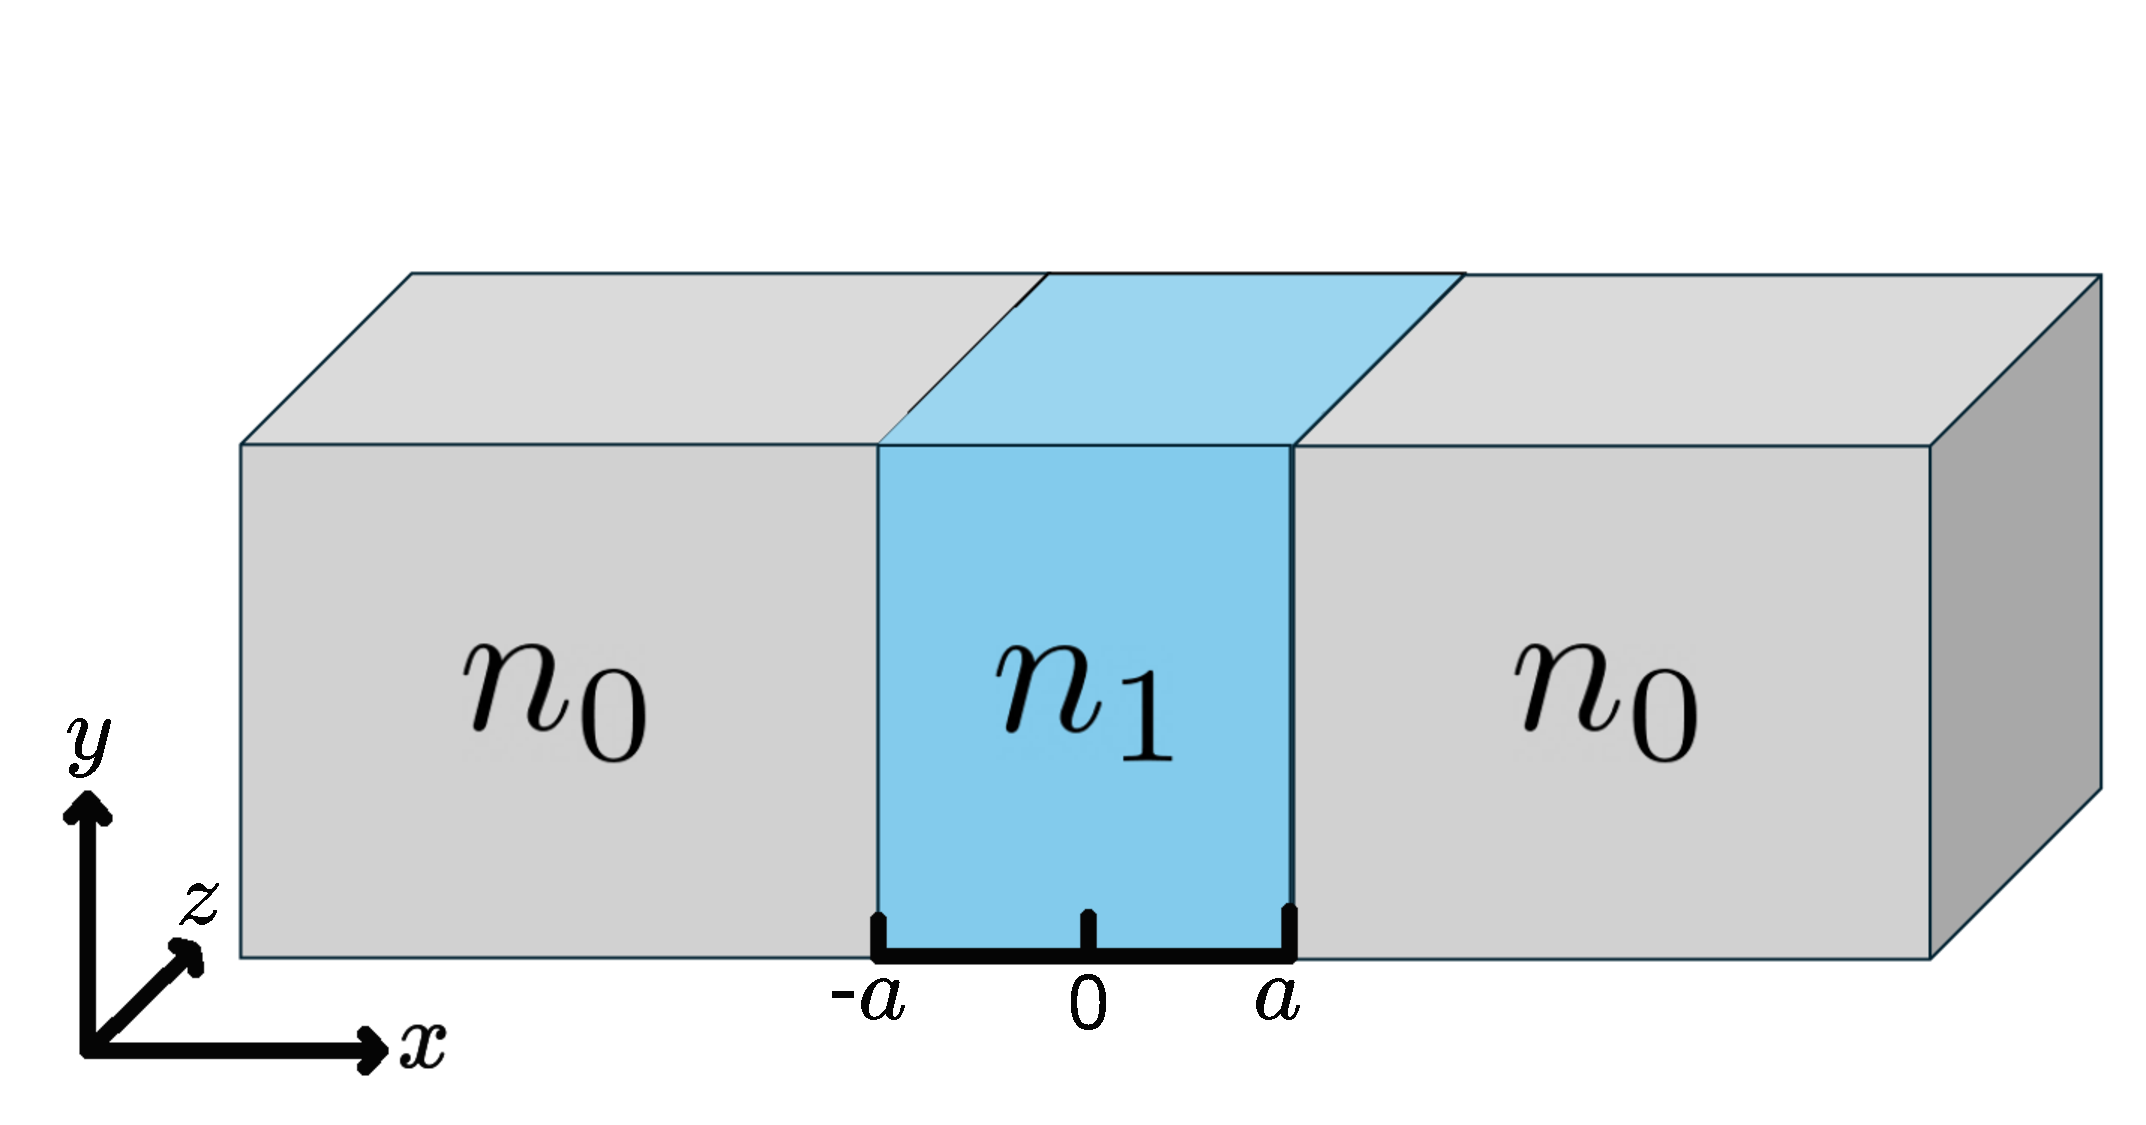
\includegraphics[width=0.6\linewidth]{media/slab.pdf}
	\caption[Shape of a slab-type waveguide.]{Shape of a slab-type waveguide. The structure is invariant in the $\mathbf{\hat{y}}$ (vertical) and $\mathbf{\hat{z}}$ (into the page) directions.}
\end{figure} Since $\nabla n^2 = \textbf{0}$ para $|x| \neq a$, the right-hand sides of equations (\ref{eqn:helmholz}) and (\ref{eqn:helmholzH}) are of the Helmholtz type. Defining $\Psi = \{E_z, H_z\} $:
\begin{align*}
	(\nabla_\perp^2  + k_0^2n^2 - k_z^2) \Psi  &=  \frac{d^2\Psi}{dx^2} + (k_0^2n^2 - k_z^2) \Psi  = 0 \ .
\end{align*}
Since $n(x)=n(-x)$, the solutions $\Psi$ must be even or odd. Indeed, if  $\Psi(x)$ is a solution, the change $x\to x'=-x$ implies that  $\Psi(-x)=\pm \Psi(x)$, since $\Psi(x)$ is a real field.
To find solutions whose energy is localized within the waveguide and decays outside it, we impose $k_0^2n_0^2 \le k_z^2 \le k_0^2n_1^2$.  It becomes natural to define $\alpha^2\equiv k_0^2n_1^2-k_z^2$ y $\beta^2\equiv k_z^2 - k_0^2n_0^2$. With all this,
\begin{equation*}
	\Psi_s = \left\{\begin{matrix}
	\Psi_{s1}\cos(\alpha x) \ , & |x|\le a
	\\
	\Psi_{s0}e^{-\beta|x|} \ , & |x|>a
	\end{matrix}\right.
	\
	\implies 	
	\	
	\nabla_\perp \Psi_s = \left\{\begin{matrix}
	-\hat{\textbf{x}}\alpha\Psi_{s1}\sin(\alpha x) \ , & |x|\le a
	\\
	-\hat{\textbf{x}}\frac{|x|}{x}\beta\Psi_{s0}e^{-\beta|x|} \ , & |x|>a
	\end{matrix}\right.
	\
	.
\end{equation*}
Thus, the even vertical components $E_y$ and $H_y$ are expressed, due to equation  (\ref{eqn:transversal}) as:
\begin{equation*}
	\begin{aligned}[c]
	 E_y &= \frac{i \omega\mu_0}{k_0^2n^2-k_z^2} \left\{\begin{matrix}
	 \alpha H_{s1}\sin(\alpha x) \ ,	 & |x|\le a
	 \\
	 \frac{|x|}{x}\beta H_{s0}e^{-\beta|x|} \ , & |x|>a
	 \end{matrix}\right.
\end{aligned} 
,\quad
	\begin{aligned}[c]
	 H_y &= \frac{-i\omega \epsilon_0 n^2}{k_0^2n^2-k_z^2} \left\{\begin{matrix}
	 \alpha E_{s1}\sin(\alpha x) \ ,	& |x|\le a
	 \\
	 \frac{|x|}{x}\beta E_{s0}e^{-\beta|x|} \ , & |x|>a
	 \end{matrix}\right.
	 \
	 .
\end{aligned} 
\end{equation*}
On the other hand, the odd solutions have the form:
\begin{equation*}
	\Psi_a = \left\{\begin{matrix}
	\Psi_{a1}\sin(\alpha x) \ , & |x|\le a
	\\
	\Psi_{a0}e^{-\beta|x|} \ , & |x|>a
	\end{matrix}\right.
	\
	\implies
	\
		\nabla_\perp \Psi_a = \left\{\begin{matrix}
	\hat{\textbf{x}}\alpha\Psi_{a1}\cos(\alpha x) \ , & |x|\le a
	\\
	-\hat{\textbf{x}}\frac{|x|}{x}\beta\Psi_{a0}e^{-\beta|x|} \ , & |x|>a
	\end{matrix}\right.
	\
	.
\end{equation*}
Therefore, Ey $E_y$ y $H_y$ are expressed as:
\begin{equation*}
	\begin{aligned}[c]
	 E_y &= \frac{i\omega\mu_0}{k_0^2n^2-k_z^2} \left\{\begin{matrix}
	 -\alpha H_{a1}\cos(\alpha x) \ , & |x|\le a
	 \\
	 \frac{|x|}{x}\beta H_{a0}e^{-\beta|x|} \ , & |x|>a
	 \end{matrix}\right.
\end{aligned} 
,\quad
	\begin{aligned}[c]
	 H_y &= \frac{i\omega \epsilon_0 n^2}{k_0^2n^2-k_z^2} \left\{\begin{matrix}
	  \alpha E_{a1}\cos(\alpha x) \ ,	 & |x|\le a
	 \\
	 -\frac{|x|}{x}\beta E_{a0}e^{-\beta|x|} \ , & |x|>a
	 \end{matrix}\right.
\end{aligned} .
\end{equation*}
By imposing continuity of the tangential components $E_y$, $E_z$, $H_y$ y $H_z$:
\begin{equation*}
	\begin{aligned}[c]
	 E_{s1}\cos(\alpha a) = E_{s0}e^{-\beta a} \ ,
	 \\	 
	 H_{s1}\cos(\alpha a) = H_{s0}e^{-\beta a} \ ,
	 \\
	 	  n_1 ^2 E_{s1}\sin(\alpha a)/\alpha = -n_0^2 E_{s0}e^{-\beta a}/\beta \ ,
	  \\
	  H_{s1}\sin(\alpha a)/\alpha = - H_{s0}e^{-\beta a}/\beta \ ,
\end{aligned} 
\quad
	\begin{aligned}[c]
		 E_{a1}\sin(\alpha a) = E_{a0}e^{-\beta a} \ ,
	 	   \\
	 H_{a1}\sin(\alpha a) = H_{a0}e^{-\beta a} \ ,
	 \\
	  n_1 ^2 E_{a1}\cos(\alpha a)/\alpha = n_0^2 E_{a0}e^{-\beta a}/\beta \ ,
	 	 \\
	  H_{a1}\cos(\alpha a)/\alpha = H_{a0}e^{-\beta a}/\beta \ .
\end{aligned} 
\end{equation*}
Seeking non-trivial solutions yields:
\begin{equation*}
	\left[\frac{\cos(\alpha a)}{\beta a} + \frac{\sin(\alpha a)}{\alpha a}\right] \left[n_0^2 \frac{\cos(\alpha a)}{\beta a} + n_1^2\frac{\sin(\alpha a)}{\alpha a} \right]
	 \left[ \frac{\sin(\alpha a)}{\beta a} - \frac{\cos(\alpha a)}{\alpha a}\right]\left[ n_0^2\frac{\sin(\alpha a)}{\beta a} - n_1^2\frac{\cos(\alpha a)}{\alpha a}\right] = 0
\end{equation*}
Two types of conditions will be distinguished:
\begin{itemize}
	\item Transverse Electric (TE) Modes:\begin{align}
	\frac{\cos(\alpha a)}{\beta a} + \frac{\sin(\alpha a)}{\alpha a}&= 0 \ , \label{eqn:TEsim}
	\\
	 \frac{\sin(\alpha a)}{\beta a} - \frac{\cos(\alpha a)}{\alpha a} &= 0 \ . \label{eqn:TEanti}
	\end{align}
	\item Transverse Magnetic (TM) Modes:\begin{align}
	n_0^2 \frac{\cos(\alpha a)}{\beta a} + n_1^2\frac{\sin(\alpha a)}{\alpha a}  &= 0 \ , \label{eqn:TMsim}
	\\
	 n_0^2\frac{\sin(\alpha a)}{\beta a} - n_1^2\frac{\cos(\alpha a)}{\alpha a} &= 0 \ . \label{eqn:TManti}
	\end{align}
\end{itemize}
Assuming $\alpha$, $\beta$ y $k_z$ are known, the amplitudes must satisfy the relations:
\begin{equation*}
	\begin{aligned}[c]
	E_{s1} \left[n_0^2 \frac{\cos(\alpha a)}{\beta a}+n_1 ^2 \frac{\sin(\alpha a)}{\alpha a}\right] = 0 \ ,
		\\
	H_{s1} \left[\frac{\cos(\alpha a)}{\beta a} + \frac{\sin(\alpha a)}{\alpha a} \right] = 0 \ ,
\end{aligned} 
\quad\quad
	\begin{aligned}[c]
	E_{a1} \left[ n_0^2\frac{\sin(\alpha a)}{\beta a} - n_1^2\frac{\cos(\alpha a)}{\alpha a}\right] = 0 \ ,
		\\
	H_{a1} \left[ \frac{\sin(\alpha a)}{\beta a} - \frac{\cos(\alpha a)}{\alpha a}\right] = 0 \ .
\end{aligned} 
\end{equation*}
The equations above impose that $E_1 = 0$ when any TE mode condition is satisfied. Similarly, the equations below impose $H_1 = 0$ in the case of TM modes, which enforces transversality in the oscillation of the respective fields.

A corollary for TE modes is that $E_z = E_x = 0$, meaning the electric field polarization will be exclusively in the $\hat{\textbf{y}}$direction. Likewise, only a beam polarized in $\hat{\textbf{x}}$ could excite a TM mode. Therefore, this must be taken into account in an experiment: an arbitrary initial condition will propagate as a linear combination of the TE and TM modes supported by the waveguide.

\subsection{Graphical Solutions and Comparison Between TE and TM Modes \label{cap:solslabTETM}}

Using the two TE mode equations along with the constraint $(\alpha a)^2 + (\beta a)^2 = k_0^2 a^2(n_1^2 - n_0^2) \equiv V^2$ it is possible to obtain graphical solutions for the propagation constants $k_z$ from the intersections $(\alpha a, \beta a)$, as plotted in Figure \ref{fig:graphTE}. The number of modes increases with the difference between refractive indices.

\begin{figure}[H]
	\centering
	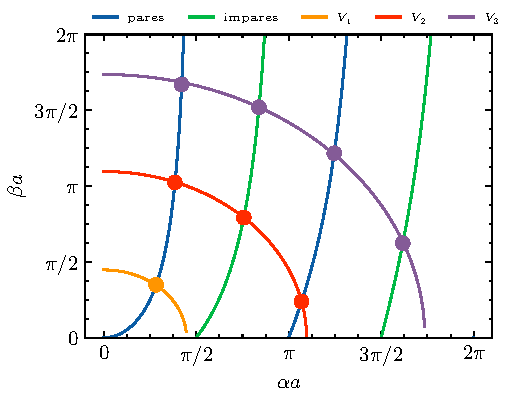
\includegraphics[width=0.5\linewidth]{media/slabgraphical.pdf}
\caption[Graphical solutions for TE modes.]{Graphical solutions for TE modes. A higher contrast $\Delta n = n_1-n_0$, results in a greater number of guided modes supported by the waveguide. \label{fig:graphTE}}
\end{figure}
After finding  $k_z$, we have everything needed to substitute into the expressions obtained for the components of the electromagnetic field. Figure \ref{fig:E-slab-graph} plots the spatial form of four modes, which correspond to the four purple points in Figure \ref{fig:graphTE}.
\begin{figure}[H]
	\centering
	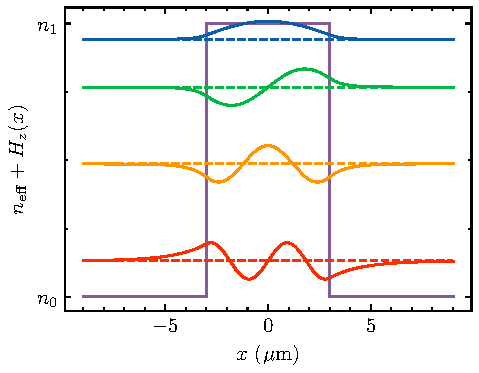
\includegraphics[width=0.5\linewidth]{media/TETMfields.pdf}
	\caption[Forma espacial de la componente longitudinal del campo magnético.]{ Spatial form of the longitudinal component of the magnetic field. \label{fig:E-slab-graph}}
\end{figure}

The cutoff condition in waveguides is equivalent to the energy no longer decaying in the region  $|x| > a$, meaning that $\beta a \to 0$ must hold.
Symmetric or even modes satisfy this condition when $\sin(V) = 0$, which implies $V = m \pi$, where $m$ is an integer. In particular, considering $m=0$  and sweeping  $n_1 \to n_0$, there are always at least two modes—one TE and one TM—as long as $n_1 > n_0$.  
Antisymmetric or odd modes, on the other hand, must satisfy $\cos(V) = 0$, which implies $V = (m\pi \pm \pi/2)$. From this condition, it follows that the first pair of excited modes ($m=0$) exists whenever $\lambda \le \lambda_c \equiv 4a\sqrt{n_1^2-n_0^2}$. Written compactly for the $m$-th mode:
\begin{align*}
	(\lambda_c)_m = \frac{4a}{m - 1} \sqrt{n_1^2 - n_0^2} \ ,
\end{align*}
which for $a=4 \text{ }\mu$m and $\Delta n = 5\times 10^{-4}$  implies a cutoff wavelength for the second mode of  $\lambda_c \approx 615 \text{ nm}$.
\section{Analytical solutions for circular optical fiber}
In the previous section, the simplest system in which dielectric waveguides can be discussed was studied. The next step in complexity involves circular waveguides. For this purpose, it will be considered that the refractive index varies radially according to:
\begin{equation}
	n( \rho ) = 
	\left\{\begin{matrix}
	n_1, \quad \text{if } \rho \le a
	\\
	n_0, \quad \text{if } \rho > a
	\end{matrix}\right.
	\ ,\nonumber
\end{equation}
where the tuple $(\rho, \phi, z)$ defines the cylindrical coordinates most appropriate for this problem.

When considering the longitudinal components $\Psi$ = $\{E_z, H_z\}$ of the electric and magnetic fields and using the method of separation of variables with $\Psi =  R(\rho)\Phi(\phi) e^{ik_z z} $,  equations (\ref{eqn:helmholz}) and (\ref{eqn:helmholzH}) take the form:
\begin{align}
	\left[\frac{\partial^2}{\partial \rho^2} + \frac{\partial}{\rho\partial \rho} + \frac{\partial^2}{\rho^2\partial \phi^2} +\left( k_0^2n^2 - k_z^2 \right)\right]  R(\rho)\Phi(\phi) = 0
	\nonumber
	\\
\rho^2\frac{d^2 R}{Rd\rho^2} + \rho\frac{dR}{Rd\rho} + \rho^2\left( k_0^2n^2 - k_z^2 \right) + \underbrace{\frac{d^2 \Phi}{\Phi d\phi^2}}_{-\ell^2} = 0
\nonumber
\end{align}
\vspace{-3em}
\begin{align}
\therefore \Phi(\phi) = A e^{i\ell\phi}
\nonumber
\end{align}
After imposing periodicity conditions  $\Phi(\phi)=\Phi(\phi + 2\pi)$, it necessarily follows that $\ell$ is an integer. Consequently, the equation for $R(\rho)$  is of the integer Bessel type. Therefore, seeking solutions such that $k_0^2 n_0^2 < \beta_z^2 < k_0^2 n_1^2$ and defining again $\alpha^2 \equiv k_0^2n_1^2 - k_z^2$ y $\beta^2\equiv k_z^2 - k_0^2n_0^2$ we have:
\begin{align}
	\frac{d^2 R}{d\rho^2} + \frac{1}{\rho}\frac{dR}{d\rho} + \left( k_0^2n^2 - k_z^2 -\frac{\ell^2}{\rho^2}\right)R  = 0
	\nonumber
	\\
	\therefore R(\rho) = 
	\left\{
	\begin{matrix}	
	C_1 J_\ell (\alpha\rho) + D_1 Y_\ell (\alpha\rho), \quad \text{if } \rho \le a  
	\\
	C_2 K_\ell (\beta\rho) + D_2 I_\ell (\beta\rho), \quad \text{if } \rho > a  
	\end{matrix}
	\right.
	\ . \nonumber
\end{align}
It is necessary to impose $D_1 = D_2 = 0$ or the solution to be finite at $\rho = 0$ and as $\rho \to +\infty$. That is, the radial part of the solution is:
\begin{align*}
 R(\rho) = 
	\left\{
	\begin{matrix}	
	C_1 J_\ell (\alpha\rho), \quad \text{if } \rho \le a  
	\\
	C_2 K_\ell (\beta\rho), \quad \text{if } \rho > a  
	\end{matrix}
	\right.
	\ . \nonumber
\end{align*}
In this case, to impose the continuity conditions on $\textbf{E}_{||} = E_\phi \boldsymbol{\hat{\phi}} + E_z \hat{\textbf{z}}$ and $\textbf{H}_{||}= H_\phi \hat{\boldsymbol{\phi}} + H_z \hat{\textbf{z}}$, it becomes necessary to relate the remaining field components to $E_z$​ and $H_z$​, for which equations (\ref{eqn:transversal}) are required.

Since 
\begin{equation*}
	\nabla_\perp \Psi =
	\left\{	
	\begin{matrix}
		\Psi_0^1\left[\boldsymbol{\hat{\rho}}\alpha J'_\ell (\alpha \rho) + i \boldsymbol{\hat{\phi}} \ell J_\ell (\alpha \rho)/\rho\right] e^{i\ell\phi} e^{i k_z z} \ , \quad \text{if } \rho \le a  
		\\
		\Psi_0^0\left[\boldsymbol{\hat{\rho}}\beta K'_\ell (\beta\rho) +i \boldsymbol{\hat{\phi}}\ell K_\ell (\alpha \rho)/\rho \right]e^{i\ell\phi} e^{i k_z z} \ , \quad \text{if } \rho > a  
	\end{matrix}
	\right.
\end{equation*}

Separating by components and substituting:
\begin{align*}
		H_z &=  e^{i\ell\phi}e^{i k_z z}
	  	 \left\{
		\begin{matrix}	  	 
	  	 H_0^1 J_\ell (\alpha \rho) \ , \quad \text{if } \rho \le a  
	  	 \\
	  	 H_0^0 K_\ell (\beta \rho) \ , \quad \text{if } \rho > a  
	  	 \end{matrix}
	  	 \right.	
		\\
	  	 H_r &= \frac{i e^{i\ell\phi}e^{i k_z z} }{k_0^2 n^2 - k_z^2}
	  	 \left\{
		\begin{matrix}	  	 
	  	  k_z \alpha H_0^1 J'_\ell (\alpha \rho) - i\omega \epsilon_0 n^2\ell E_0^1 J_\ell (\alpha \rho)/\rho \ , \quad \text{if } \rho \le a  
	  	 \\
	  	 k_z \beta H_0^0  K'_\ell (\beta \rho) - i\omega \epsilon_0 n^2\ell E_0^0 K_\ell (\beta \rho)/\rho \ , \quad \text{if } \rho > a  
	  	 \end{matrix}
	  	 \right.
	  	 \\
		H_\phi &= \frac{ie^{i\ell\phi} e^{i k_z z}}{k_0^2 n^2 - k_z^2}
		\left\{
		\begin{matrix}
			ik_z\ell H_0^1  J_\ell (\alpha \rho)/\rho + \omega \epsilon_0 n^2  \alpha E_0^1 J'_\ell (\alpha \rho) \ , \quad \text{if } \rho \le a  
			\\
			ik_z \ell H_0^0  K_\ell (\beta \rho)/\rho + \omega \epsilon_0 n^2 \beta E_0^0  K'_\ell (\beta \rho) \ , \quad \text{if } \rho > a  
		\end{matrix}
		\right.
		\\
		E_z &= e^{i\ell\phi} e^{i k_z z}
	  	 \left\{
		\begin{matrix}	  	 
	  	 E_0^1 J_\ell (\alpha \rho) \ , \quad \text{if } \rho \le a  
	  	 \\
	  	 E_0^0 K_\ell (\beta \rho) \ , \quad \text{if } \rho > a  
	  	 \end{matrix}
	  	 \right.	
		\\
	E_r &= \frac{i e^{i\ell\phi} e^{i k_z z} }{k_0^2 n^2 - k_z^2}
	  	 \left\{
		\begin{matrix}	  	 
	  	  k_z \alpha E_0^1 J'_\ell (\alpha \rho)+i\omega \mu_0 \ell H_0^1 J_\ell (\alpha \rho)/\rho \ , \quad \text{if } \rho \le a  
	  	 \\
	  	 k_z \beta E_0^0  K'_\ell (\beta \rho) +i\omega \mu_0 \ell H_0^0 K_\ell (\beta \rho)/\rho \ , \quad \text{if } \rho > a  
	  	 \end{matrix}
	  	 \right.
	\\
	E_\phi &= \frac{i e^{i\ell\phi} e^{i k_z z}}{k_0^2 n^2 - k_z^2}
		\left\{
		\begin{matrix}
			ik_z \ell E_0^1   J_\ell (\alpha \rho)/\rho -\omega \mu_0  \alpha H_0^1  J'_\ell (\alpha \rho) \ , \quad \text{if } \rho \le a  
			\\
			ik_z \ell E_0^0   K_\ell (\beta \rho)/\rho -\omega \mu_0 \beta H_0^0   K'_\ell (\beta \rho) \ , \quad \text{if } \rho > a  
		\end{matrix}
		\right.
\end{align*}
Then, imposing continuity in $z$ and $\phi$:
\begin{align}
	H_0^{1} J_\ell(\alpha a) &= H_0^{0} K_\ell (\beta a)
	\label{eqn:cont1}
	\\
	E_0^{1} J_\ell(\alpha a) &= E_0^{0} K_\ell (\beta a)
	\label{eqn:cont2}
	 \\
	 -\omega \epsilon_0 n_1^2  \alpha\beta^2 a E_0^1 J'_\ell (\alpha a)-ik_z\ell \beta^2 H_0^1  J_\ell (\alpha a)
	 &= \omega \epsilon_0 n_0^2 \alpha^2 \beta a E_0^0 K'_\ell (\beta a)+ik_z\ell \alpha^2H_0^0  K_\ell (\beta a)
	 \label{eqn:cont3}
	 \\
	 -ik_z \ell \beta^2 E_0^1   J_\ell (\alpha a) + \omega \mu_0  \alpha \beta^2 a H_0^1  J'_\ell (\alpha a) &=
	 ik_z \ell \alpha^2 E_0^0   K_\ell (\beta a) -\omega \mu_0  \alpha^2 \beta a H_0^0  K'_\ell (\beta a)
	 \label{eqn:cont4}
\end{align}
Seeking non-trivial solutions:
\begin{align*}
	\left|\begin{matrix}
		K_\ell(\beta a) & -J_\ell(\alpha a) & 0 & 0
		\\
		0 & 0 & K_\ell(\beta a) & -J_\ell(\alpha a)
		\\
		ik_z\ell \alpha^2 K_\ell (\beta a) & ik_z\ell\beta^2 J_\ell (\alpha a) & \omega \epsilon_0 n_0^2  \alpha^2 \beta a K'_\ell (\beta a) & \omega \epsilon_0 n_1^2  \alpha \beta^2 a J'_\ell (\alpha a)
		\\
		\omega \mu_0  \alpha^2 \beta a   K'_\ell (\beta a) &  \omega \mu_0  \alpha \beta^2 a J'_\ell (\alpha a) & -ik_z \ell \alpha^2 K_\ell (\beta a) &  -ik_z \ell \beta^2  J_\ell (\alpha a)
	\end{matrix}\right|
	=
0
\end{align*}
Finally, the transcendental equation satisfied by  $\alpha$, $\beta$ and $k_z$ is:
\begin{equation}
	\left( \frac{J_\ell'(\alpha a)}{\alpha a J_\ell(\alpha a)} + \frac{K_\ell'(\beta a)}{\beta a K_\ell(\beta a)} \right)\left( n_1^2\frac{J_\ell'(\alpha a)}{\alpha a J_\ell(\alpha a)} + n_0^2\frac{K_\ell'(\beta a)}{\beta a K_\ell(\beta a)} \right) = \ell^2 \left[ \left(\frac{1}{\alpha a}\right)^2 + \left(\frac{1}{\beta a}\right)^2 \right]^2 \left( \frac{k_z}{k_0} \right)^2 . \label{eqn:fiber_trascendental}
\end{equation}
Since, in principle, the values of $k_z$ are already determined by the equation above, it is possible to obtain two relations between $H_0^1$ and $E_0^1$:
\begin{align}
\frac{E_0^1}{H_0^1} &=  -\frac{i k_z \ell}{\omega\epsilon_0}\left[ \left(\frac{1}{\alpha a}\right)^2 + \left(\frac{1}{\beta a}\right)^2 \right]  \left[ n_1^2 \frac{J'_\ell(\alpha a)}{\alpha a J_\ell(\alpha a)} + n_0^2 \frac{K'_\ell(\beta a)}{\beta a K_\ell(\beta a)} \right]^{-1} \label{eqn:fiber_polarization_E},
\\
\frac{H_0^1}{E_0^1} &=  \frac{i k_z \ell}{ \omega\mu_0}\left[ \left(\frac{1}{\alpha a}\right)^2 + \left(\frac{1}{\beta a}\right)^2 \right]  \left[ \frac{J'_\ell(\alpha a)}{\alpha a J_\ell(\alpha a)} + \frac{K'_\ell(\beta a)}{\beta a K_\ell(\beta a)} \right]^{-1} \label{eqn:fiber_polarization_H}.
\end{align}
Taking the square root of the quotient of the equations: (\ref{eqn:fiber_polarization_E}) ans (\ref{eqn:fiber_polarization_H}) we have:
\begin{equation}
	\frac{E_0^1}{H_0^1} = i \sqrt{\frac{\mu_0}{\epsilon_0}} \frac{\sqrt{ \frac{J'_\ell(\alpha a)}{\alpha a J_\ell(\alpha a)} + \frac{K'_\ell(\beta a)}{\beta a K_\ell(\beta a)}}}{\sqrt{n_1^2 \frac{J'_\ell(\alpha a)}{\alpha a J_\ell(\alpha a)} + n_0^2 \frac{K'_\ell(\beta a)}{\beta a K_\ell(\beta a)}}} \ .
	\label{eqn:fiber_polarization_simplified}
\end{equation}
\subsection{TE and TM modes}
The simplest case to study is by imposing $\ell = 0$. Equation (\ref{eqn:fiber_trascendental}) implies:
\begin{align*}
	\frac{J'_{0}(\alpha a)}{\alpha a J_0(\alpha a)} + \frac{K'_0(\beta a)}{\beta a K_0(\beta a)}&=  0 \ , \quad \text{(TE modes)}
	\\
	n_1^2\frac{J'_{0}(\alpha a)}{\alpha a J_0(\alpha a)} + n_0^2 \frac{K'_0(\beta a)}{\beta a K_0(\beta a)} &= 0 \ , \quad \text{(TM modes)}
\end{align*}
from equation (\ref{eqn:fiber_polarization_simplified}), it is straightforward to note that the conditions for transverse modes imply that the longitudinal components become zero in the respective cases: $H_0^1 = 0$for TE and $E_0^1 = 0$ for TM.

The cutoff conditions occur when $\beta a \to 0$. Using the asymptotic expressions for Bessel functions with small arguments and their recurrence relations, we have:
\begin{align*}
	\frac{\alpha a J_0(\alpha a)}{J_1(\alpha a)}  = -\frac{\beta a K_{0}(\beta a)} {K_1(\beta a)} \approx (\beta a)^2\ln\left(\frac{\beta a e^\gamma}{2}\right) \to 0 \ ,
\end{align*}
thus it becomes necessary that $\left. J_0(\alpha a)\right|_{\alpha a \to V} = 0$. Denoting $x_{0,m}=$ 2.405,  5.520,  8.654, $\cdots$ as the  $m$-th zero of the function $J_0(x)$, the cutoff wavelength is given by:
\begin{equation}
(\lambda_c)_{0,m} = 2\pi a \frac{\sqrt{n_1^2 - n_0^2}}{x_{0,m}} \ , \quad\text{(TE and TM modes)},
\end{equation} 
which translates to a cutoff wavelength of: $\lambda_c\approx 616$ nm for the same parameters as in the section \ref{cap:slab}, $a=4 \text{ }\mu$m y $\Delta n = 5\times 10^{-4}$ . Contrary to the case of slab waveguides, in optical fibers it is necessary to be below a non-zero maximum cutoff threshold $(\lambda_c)_{0,1}$ for TE or TM modes to exist. As will be seen later, this is because purely transverse modes correspond to excited modes: the fundamental mode is hybrid.


%\begin{figure}[H]
%	\centering
%	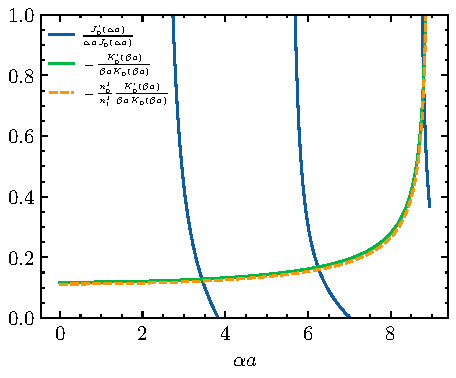
\includegraphics[width=0.7\linewidth]{media/fibergraphical}
%\end{figure}

\subsection{HE and EH modes}
Interpreting (\ref{eqn:fiber_trascendental}) as a quadratic equation in $J_\ell'(\alpha a)/\alpha a J_\ell(\alpha a)$:
\begin{align*}
	\frac{J_\ell'(\alpha a)}{\alpha a J_\ell(\alpha a)} &= -\left(\frac{n_1^2+n_0^2}{2n_1^2}\right) \frac{K_\ell'(\beta a)}{\beta a K_\ell(\beta a)}\pm\sqrt{\left(\frac{n_1^2-n_0^2}{2n_1^2}\right)^2\left(\frac{K_\ell'(\beta a)}{\beta a K_\ell(\beta a)}\right)^2+ \left( \frac{ k_z \ell}{ k_0 n_1} \right)^2\left[ \left(\frac{1}{\alpha a}\right)^2 + \left(\frac{1}{\beta a}\right)^2 \right]^2 }
\end{align*}

If the recurrence relations of the Bessel functions $J_\ell(r)$,are used, it is possible to obtain two types of solutions that are usually called HE and EH due to the longitudinal field with greater relative value:
\begin{align}
		\frac{J_{\ell-1}(\alpha a)}{\alpha a J_\ell(\alpha a)} &= -\left(\frac{n_1^2+n_0^2}{2n_1^2}\right) \frac{K_\ell'(\beta a)}{\beta a K_\ell(\beta a)}+\frac{\ell}{(\alpha a)^2}-\sqrt{\Delta} \ , \quad \text{(HE modes)}
		\label{eqn:HE}
	\\
		\frac{J_{\ell+1}(\alpha a)}{\alpha a J_\ell(\alpha a)} &= \left(\frac{n_1^2+n_0^2}{2n_1^2}\right) \frac{K_\ell'(\beta a)}{\beta a K_\ell(\beta a)}+\frac{\ell}{(\alpha a)^2}-\sqrt{\Delta} \ , \quad \text{(EH modes)}
		\label{eqn:EH}
		\\
		\Delta &= \left(\frac{n_1^2-n_0^2}{2n_1^2}\right)^2\left(\frac{K_\ell'(\beta a)}{\beta a K_\ell(\beta a)}\right)^2+ \left( \frac{ k_z \ell}{ k_0 n_1} \right)^2\left[ \left(\frac{1}{\alpha a}\right)^2 + \left(\frac{1}{\beta a}\right)^2 \right]^2 \ . \nonumber
\end{align}
For $\ell = 0$,  the relations obtained for the TE$_m$ (HE$_{0m}$) and TM$_m$ (EH$_{0m}$). For $\ell \neq 0$ it becomes necessary to consider the asymptotic expressions of the Bessel functions when $\beta a \to 0$ and $\alpha a \to V$:
\begin{align*}
	\frac{K'_\ell (x)}{xK_\ell (x)} &= -\frac{K_{\ell-1} (x)}{xK_\ell (x)}-\frac{\ell}{x^2}\approx \left\{\begin{matrix}
	\ln(xe^\gamma/2)-\frac{1}{x^2} \quad\text{si }\ell = 1
	\\
	-\frac{
	1}{2(\ell-1)}-\frac{\ell}{x^2}\quad \text{si }\ell > 1
	\end{matrix}\right. .
\end{align*}
The case $\ell=1$ is of special interest. The condition for HE modes is developed as:
\begin{align*}
	\frac{\alpha a J_1(\alpha a)}{J_0(\alpha a)} &= \left\{\left(\frac{n_1^2+n_0^2}{2n_1^2}\right) \left[ \ln\left(\frac{2}{e^\gamma \beta a}\right)+\frac{1}{(\beta a)^2} \right]+\frac{1}{(\alpha a)^2}-\sqrt{\Delta}\right\}^{-1} \to 0 \ .
\end{align*}
It is sufficient to consider the function $J_1(\alpha a)|_{\alpha a \to V} = 0$. On the other hand, the EH condition eliminates the zero $x=0$ from the ratio $\frac{\alpha aJ_1(\alpha a)}{J_2(\alpha a)}$ which causes it to be "out of phase" relative to the HE condition. Using reasoning similar to the $\ell =0$, case, the cutoff conditions are:
\begin{align*}
	(\lambda_c)_{1,m} &= 2\pi a \frac{\sqrt{n_1^2 - n_0^2}}{x_{1,m}} \ ,  \quad \left(\text{HE modes}_{1m}\right)
	\\
	(\lambda_c)_{1,m} &= 2\pi a \frac{\sqrt{n_1^2 - n_0^2}}{x_{1,m+1}} \ , \quad \left(\text{EH modes}_{1m}\right)
\end{align*}
with $x_{1,m}=$ 0, 3.832,  7.016, 10.173, $\dots$. In particular, the $\text{HE}_{11}$ mode always exists. The next largest finite cutoff wavelengths are $\lambda_c \approx 252$ nm for the $\text{HE}_{12}$ and $\text{EH}_{11}$ modes.

The case $\ell \ge 2$ has a different development due to the asymptotic forms involved and will not be relevant for this thesis. However, they are included in Figure \ref{fig:vortices} for completeness.
\begin{figure}[H]
	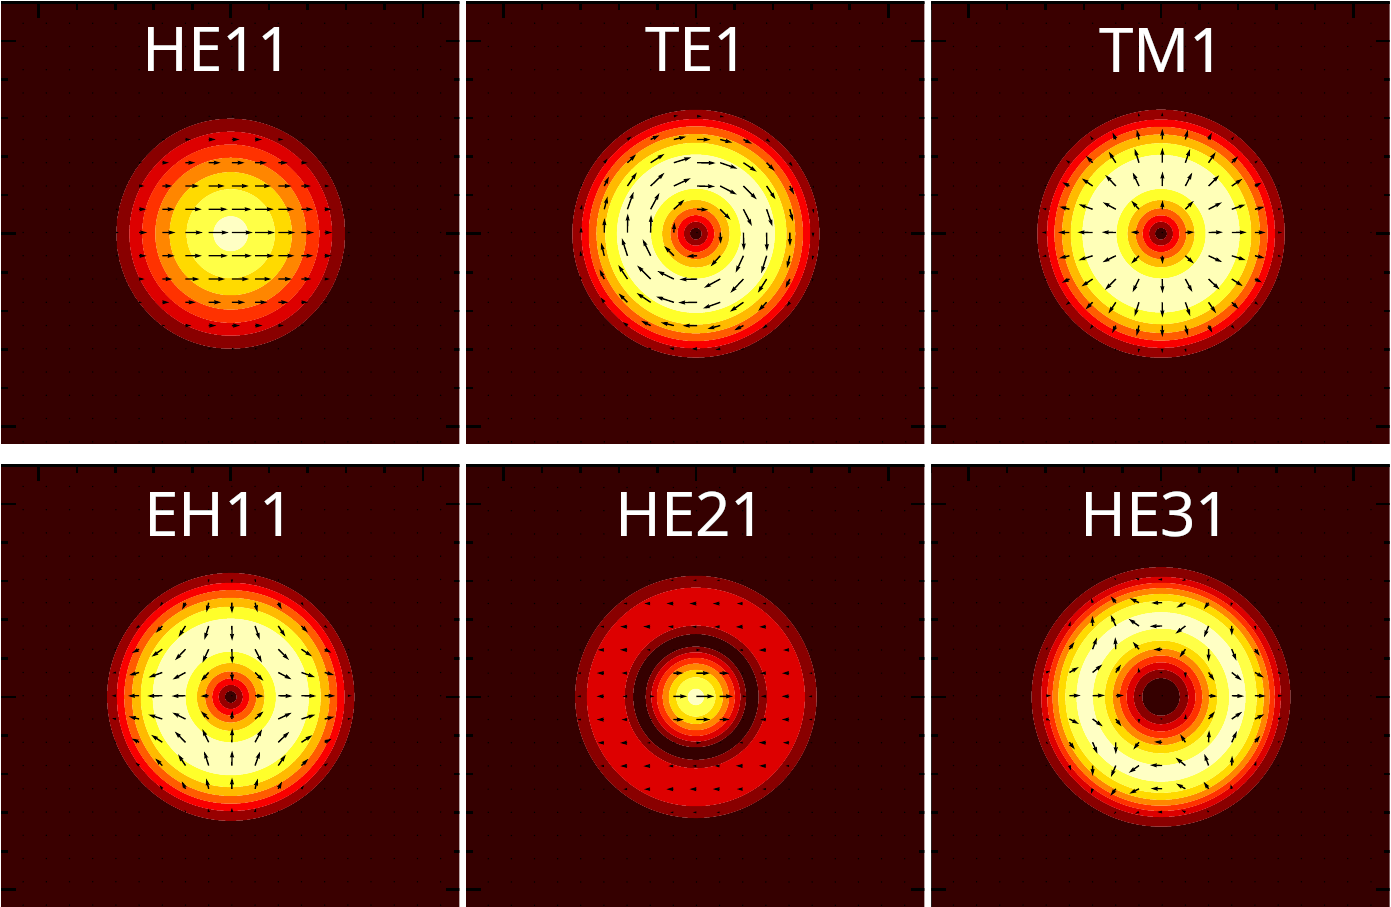
\includegraphics[width=\linewidth]{media/OAM_analitic}
		\caption{First guided normal modes for a circular waveguide or optical fiber. \label{fig:vortices}}
\end{figure}

\section{Normal modes in waveguides}

If the waveguide structure does not vary in the  \( \hat{\textbf{z}} \)direction, the solution for the electric field can be written, by separation of variables, as a plane wave of the form \( \textbf{E}(\textbf{r}) = \textbf{E}_\nu(x, y) e^{i\beta_\nu z} \). In turn, it is convenient to separate the Laplacian operator as \( \nabla^2 = \nabla_\perp^2 + \frac{\partial^2}{\partial z^2} \). 

Defining the operator \( D_{ij} \) such that  \( D_{ij} E_j \equiv \partial_i\left(\frac{\partial_j n^2}{n^2}E_j \right) \), he transverse part of the Helmholtz equations (\ref{eqn:helmholz}) can be written as:
\begin{align}
	\begin{pmatrix}
		\nabla_\perp^2  + k_0^2n^2 + D_{xx} & D_{xy} 
		\\
		D_{yx}  & \nabla_\perp^2  + k_0^2n^2 + D_{yy} 
	\end{pmatrix}
	\begin{pmatrix}
		E_x
		\\
		E_y
	\end{pmatrix}
	=
	\beta_\nu^2 
	\begin{pmatrix}
		E_x
		\\
		E_y
	\end{pmatrix} \ . \label{eqn:eigenfield}
\end{align}

Equation (\ref{eqn:eigenfield}) constitutes an eigenvalue problem for \( \beta_\nu^2 \), whose eigenfunctions \( \textbf{E}_\nu^\perp(x,y) \) d describe the transverse profiles of the guided modes. In general, this is a coupled vectorial second-order system, whose resolution requires numerical techniques. However, in the \textit{weak guidance} regime, where the refractive index varies slightly relative to a homogeneous background  \( n_0 \), the system can be decoupled and treated as a scalar problem for a dominant component of the electric field\footnote{see \ref{sec:orto}.}.

Under this approximation, quasi-transverse modes are typically considered, where the electric field is primarily polarized in a fixed direction (for example, \( E_y \)), and the Helmholtz equation reduces to:
\begin{equation}
	\left[\nabla_\perp^2 + k_0^2 n^2(x,y) \right] \phi_\nu(x,y) = \beta_\nu^2 \phi_\nu(x,y) \ ,
\end{equation}
where \( \phi_\nu(x,y) \) represents the transverse field profile. This approximation is valid for many experimental geometries, especially when the light is linearly polarized and the index variations do not induce coupling between orthogonal polarizations.

The modes obtained from this equation allow for the calculation of propagation constants \( \beta_\nu \), spatial field profiles \( \phi_\nu(x,y) \), and other relevant quantities such as confinement factors or group velocities. Furthermore, these modes serve as a basis for subsequent numerical methods, such as Eigenmode Expansion (EME) or Coupled-Mode Theory (CMT), used to describe the dynamics in photonic lattices.
\section{Coupled-Mode Theory \label{cap:CMTteo}}
\subsection{Derivation from a Variational Principle}

From equations (\ref{eqn:EfieldH}) and (\ref{eqn:HfieldE}), it is possible to express the propagation constant $k_z$ in terms of the Poynting vector $\textbf{S} = \frac{1}{2} \text{Re}\{\textbf{E} \times \textbf{H}^*\}$, following a derivation analogous to that presented in \citep{haus_coupled-mode}. 
\begin{equation}
	k_z = \frac{
		\frac{1}{4i} \iint \left[
		\left(-\nabla_\perp \times \textbf{E} + i\omega \mu_0 \textbf{H}\right) \cdot \textbf{H}^* 
		+ \left(\nabla_\perp \times \textbf{H} + i\omega \varepsilon_0 n^2 \textbf{E}\right) \cdot \textbf{E}^*
		\right] dxdy
	}{
		\frac{1}{4} \iint \left( 
		\textbf{E} \times \textbf{H}^* + \textbf{E}^* \times \textbf{H}
		\right) \cdot \hat{\textbf{z}} \, dxdy
	} \ . 
	\label{eqn:kzprevar}
\end{equation}
When proposing a solution in the form of a superposition of modes from the individual waveguides, such as:
\begin{align*}
	\textbf{E} &= \sum_i a_i \textbf{e}_i \ , \quad \textbf{H} = \sum_i a_i \textbf{h}_i \ ,
\end{align*}
where $a_i$ represents the amplitude of the $i$-th mode, the coefficients remain undetermined but subject to minimizing the expression for $k_z$. Substituting these expansions into (\ref{eqn:kzprevar}), a simplified expression for the propagation constant of the system $k_z$ is obtained:
\begin{align*}
	(\textbf{E}\times\textbf{H}^* + \textbf{E}^*\times\textbf{H})\cdot\hat{\textbf{z}} 
	&= \sum_{ij} a_i^* \left( \textbf{e}_j \times \textbf{h}_i^* + \textbf{e}_i^* \times \textbf{h}_j \right) \cdot \hat{\textbf{z}} \, a_j 
	\equiv \sum_{ij} a_i^* p_{ij} a_j \ .
\end{align*}
The integrand of the numerator is expanded as:
\begin{align*}
	\text{integrand of the numerator} &= i\sum_{ij} \Big[ a_i^* k_z^j (\hat{\textbf{z}}\times\textbf{e}_j )\cdot\textbf{h}_i^* a_j  + a_j \left(\omega \varepsilon_0 (n^2-n_j^2) \textbf{e}_j - k_z^j \hat{\textbf{z}}\times\textbf{h}_j \right) \cdot \textbf{e}_i^* a_i^* \Big] \ , \\
	&= i\sum_{ij} a_i^* \left[ k_z^j p_{ij} + \omega \varepsilon_0(n^2-n_j^2) \textbf{e}_j \cdot \textbf{e}_i^* \right] a_j \ ,
\end{align*}
where $k_z^j$ is the propagation constant of the $j$-th isolated mode\footnote{in general, $k_z \neq k_z^j$.}. 

Defining the following fundamental quantities:
\begin{align}
	P_{ij} &\equiv \frac{1}{4} \iint \left( \textbf{e}_j \times \textbf{h}_i^* + \textbf{e}_i^* \times \textbf{h}_j \right) \cdot \hat{\textbf{z}} \ , dxdy, \label{eqn:pij-ori} \\
	&= \frac{1}{4 \omega \mu_0} \iint \Big[ 
	(k_z^i + k_z^j) \left( \textbf{e}_i^* \cdot \textbf{e}_j - e_{z,i}^* e_{z,j} \right)  + i \left( \textbf{e}_i^* \cdot \nabla_\perp e_{z,j} + \textbf{e}_j \cdot \nabla_\perp e_{z,i}^* \right) \Big] dxdy \ , \label{eqn:pij-simpli} \\
	H_{ij} &\equiv P_{ij} k_z^j + \frac{\omega \varepsilon_0}{4} \iint (n^2-n_j^2) \textbf{e}_j \cdot \textbf{e}_i^* \, dxdy \ , \label{eqn:hij}
\end{align}
the expression (\ref{eqn:kzprevar}) for the propagation constant $k_z$ can be written compactly as a Rayleigh-Ritz quotient:
\begin{equation}
	k_z = \frac{\sum_{ij} a_i^* H_{ij} a_j}{\sum_{ij} a_i^*P_{ij} a_j} \ .
\end{equation}
Differentiating with respect to $a_k^*$ to optimize the value of $k_z$ yields:
\begin{align}
	\frac{\partial k_z}{\partial a_k^*} &= \frac{\sum_{ij} H_{ij} a_j \delta_{ik}}{\sum_{ij} a_i^*P_{ij} a_j} - \frac{\left(\sum_{ij} a_i^* H_{ij} a_j\right) \left( 
	\sum_{ij} \delta_{ik} P_{ij} a_j \right) }{\left(\sum_{ij} a_i^*P_{ij} a_j\right)^2} = \frac{\sum_{j} \left(H_{jk}  - k_z P_{kj} \right) a_j}{\sum_{ij} a_i^* P_{ij}a_j} \overset{!}{=} 0 \ .
\end{align}
Recovering $k_z \to -i\frac{\partial}{\partial z}$, the equations for $N$ non-orthogonal coupled modes are obtained:
\begin{equation}
	-i \sum_{j} P_{kj} \frac{d a_j}{dz} ´= \sum_{j} H_{kj} a_j \ , \text{ with }k=1,2,\cdots,N \ . \label{eqn:non-ortho-CMT-eqs}
\end{equation}
Clearly, from the expression (\ref{eqn:pij-ori}) for $P_{ij}$, Hermiticity is satisfied. At first glance, it may seem that $H_{ij}$ is not Hermitian, but let us see that it indeed is. To do this, it suffices to consider the difference $H_{ij} - H_{ji}^*$ and note that it vanishes:
\begin{align*}
 H_{ij} - H_{ji}^* &= P_{ij} k_z^j - P_{ji}^* k_z^i  + \frac{\omega \varepsilon_0}{4} \iint(n_i^2-n_j^2) \textbf{e}_i^* \cdot \textbf{e}_j dxdy
\\
&= \frac{1}{4} \iint (k_z^j-k_z^i)( \textbf{e}_j \times  \textbf{h}_i^* + \textbf{e}_i^* \times  \textbf{h}_j  )\cdot\hat{\textbf{z}} + \omega\varepsilon_0 (n_i^2-n_j^2) \textbf{e}_j \cdot \textbf{e}_i^* dxdy
\\
&= \frac{1}{4} \iint \left( i\nabla_\perp \times \textbf{e}_j +\omega\mu_0 \textbf{h}_j \right) \cdot \textbf{h}_i^* - \left( i\nabla_\perp \times \textbf{h}_j  - \omega\varepsilon_0n_j^2 \textbf{e}_j \right) \cdot \textbf{e}_i^*dxdy
\\
&- \frac{1}{4} \iint \left( i\nabla_\perp \times \textbf{e}_i^* +\omega\mu_0 \textbf{h}_i^*\right) \cdot \textbf{h}_j + \left(i\nabla_\perp \times \textbf{h}_i^*  + \omega\varepsilon_0n_i^2 \textbf{e}_i^* \right) \cdot \textbf{e}_jdxdy
\\
&+\frac{\omega\varepsilon_0}{4}\iint  \left(n_i^2-n_j^2\right) \textbf{e}_j \cdot \textbf{e}_i^* dxdy
\\
&= \frac{i}{4} \iint \left(\nabla_\perp\times\textbf{e}_j\right) \cdot \textbf{h}_i^*  -\left(\nabla_\perp\times\textbf{h}_j\right) \cdot \textbf{e}_i^* + \left(\nabla_\perp\times\textbf{e}_i^*\right) \cdot \textbf{h}_j - \left(\nabla_\perp\times\textbf{h}_i^*\right) \cdot \textbf{e}_j dxdy
\\
&= \frac{i}{4} \iint \nabla_\perp\cdot\left(\textbf{e}_j \times \textbf{h}_i^* +\textbf{e}_i^* \times \textbf{h}_j\right) dxdy =
\frac{i}{4} \oint_C \left(\textbf{e}_j \times \textbf{h}_i^* +\textbf{e}_i^* \times \textbf{h}_j\right) \cdot \hat{\textbf{n}} ds
\\
&=
0 \ ,
	\end{align*}
where it has been used that the fields must decay to zero at infinity. Equations (\ref{eqn:non-ortho-CMT-eqs}) can be derived from a Principle of Least Action after defining the discrete field Lagrangian $L$ of the Schrödinger type:
\begin{equation}
	L = -\sum_{ij}  a_i^*\left(i  P_{ij} \frac{d }{dz} + H_{ij}  \right)a_j \ .
\end{equation}
The generalized momenta of this Lagrangian are $\Pi_k=\frac{\partial L}{\partial \dot{a_k}} = -i\sum_{j} a_j^* P_{jk}$, so the associated Hamiltonian $H$ is:
\begin{equation}
H = \sum_{j} \Pi_j \dot{a_j} - L = \sum_{ij} -ia_i^* P_{ij} \dot{a_j} + a_i^*\left(i  P_{ij} \frac{d a_j}{dz} + H_{ij} a_j \right) = \sum_{ij} a_i^* H_{ij} a_j \ .
\end{equation}
Since the Lagrangian does not depend explicitly on $z$, the Hamiltonian $H$ is a conserved quantity. Varying the Lagrangian yields:
\begin{align*}
	\delta L &= \sum_{ij} \frac{\partial L}{\partial a_j} \delta a_{j} +  \frac{\partial L}{\partial {a}_{i}^*} \delta {a}_{i}^* + \ \frac{\partial L}{\partial \dot{a}_{j}} \delta \dot{a}_{j} + \frac{\partial L}{\partial \dot{{a}}_{i}^*} \delta \dot{{a}}_{i}^*
	\\
	&= \sum_{ij} \left( \frac{\partial L}{\partial a_{j}} - \frac{d}{dz}\frac{\partial L}{\partial \dot{a}_{j}} \right)\delta a_{j} + \left( \frac{\partial L}{\partial {a}_{i}^*} - \frac{d}{dz}\frac{\partial L}{\partial  \dot{{a}}_{i}^*} \right)\delta {a}_{i}^* + \frac{d}{dz}\left(\frac{\partial L}{\partial \dot{a}_{j}}\delta a_{j} +  \frac{\partial L}{\partial \dot{{a}}^*_{i}}\delta {a}_{i}^*\right)
	\\	
	&\implies  \frac{d}{dz} \sum_{ij}\left(\frac{\partial L}{\partial \dot{a}_{j}}\delta a_{j} +  \frac{\partial L}{\partial \dot{{a}}_{i}^*}\delta {a}_{i}^*\right) = 0 \ .
\end{align*}
The pair of transformations associated with the unitary group U(1), $a_j\to a'_j = e^{i\phi}a_j$, ${a}_i^* \to {a'}_i^* = e^{-i\phi}{a}_i^*$ leave the Lagrangian invariant. If an infinitesimal variation $\phi \ll 1$ is taken, then $\delta a_j = i\phi a_j$ and $\delta {a}_i^* = -i\phi {a}_i^*$, is taken, then $P$, which is identified with the total power of the system and is directly related to the Poynting vector, is:
\begin{equation}
	P = \sum_{ij} a_i^* P_{ij} a_j = \iint \textbf{S} \cdot \hat{\textbf{z}} dxdy \ .  \label{eqn:power}
\end{equation}
Thus, there are two conserved quantities in the dynamics, $H$ y $P$, which will be useful for verifying the validity of numerical solutions to equation (\ref{eqn:non-ortho-CMT-eqs}).

\subsection{TE Dimer in Slab-Type Waveguides}
Using the equations for the transverse components (\ref{eqn:transverse}) in the case of fundamental TE modes (\ref{eqn:TEanti}), we have:
\begin{align*}
	\textbf{e}_{j\perp} &= \hat{\textbf{y}}\frac{i\omega\mu_0 H_{a1}}{k_0^2n_j^2 - (k_z^j)^2}\left\{ \begin{matrix}
-\alpha \cos(\alpha (x-x_j)), &|x-x_j|\le a
\\
\beta\sin(\alpha a) e^{-\beta(|x-x_j|-a)}, &|x-x_j| > a
\end{matrix}\right. \ ,
\\
\textbf{h}_{j\perp} &= \hat{\textbf{x}}\frac{ik_z^j H_{a1}}{k_0^2n_j^2 - (k_z^j)^2}\left\{ \begin{matrix}
\alpha \cos(\alpha (x-x_j)), &|x-x_j|\le a
\\
-\beta\sin(\alpha a) e^{-\beta(|x-x_j|-a)}, &|x-x_j| > a
\end{matrix}\right. \ ,
\end{align*} with $x_j=jd$, $d\ge 2a$ and $L=\int dy$. The off-diagonal elements have the form:
\begin{align*}
	\left(\textbf{e}_{j\perp}\times\textbf{h}_{i\perp}^*\right)\cdot \hat{\textbf{z}}
	&=
	\frac{k_z^i \omega \mu_0 H_{a1}^2 \beta\sin(\alpha a)}{(k_0^2n_j^2 - k_z^2)(k_0^2n_i^2 - k_z^2)}
	\left\{
	\begin{matrix}
		 \alpha\cos(\alpha(x-x_i))e^{-\beta(|x-x_j|-a)}, & |x-x_i| \le a
		\\
		i \leftrightarrow j, & |x-x_j| \le a
		\\
		\beta \sin(\alpha a)e^{-\beta (|x-x_i|+|x-x_j|-2a)}, & \text{otherwise}
	\end{matrix}
	\right. \ ,
\\
	P_{ij} &= \frac{L k_z^i k_0  \mu_0 c H_{a1}^2 \sin^2(\alpha a)e^{-\beta d}e^{\beta a}}{2\beta} \left[\frac{e^{-\beta a} + \beta (d-2a)e^{\beta a}}{\beta^2} - \frac{2\cosh(\beta a)}{\alpha^2+\beta^2} \right] \ ,
\\
	\tilde{H}_{ij} &\equiv H_{ij} - P_{ij} k_z^j = \frac{L k_0    \mu_0 c H_{a1}^2 }{2 \beta }  \sin^2(\alpha a)e^{2\beta a} e^{-\beta d} \ .
\end{align*}
The diagonal elements have the form:
\begin{align*}
	\left(\textbf{e}_{j\perp}\times\textbf{h}_{j\perp}^*\right)\cdot \hat{\textbf{z}}&=\frac{k_z^j\omega\mu_0 H_{a1}^2}{(k_0^2n_j^2-k_z^2)^2} \left\{ \begin{matrix}
\alpha^2\cos^2(\alpha (x-x_j)), & |x-x_j| \le a
\\
\beta^2 \sin^2(\alpha a) e^{2\beta a} e^{-2\beta|x-x_j|}, & |x-x_j|>a
\end{matrix}\right. \ ,
\\
	P_{jj} &= \frac{L k_z^j  k_0 \mu_0 c H_{a1}^2  a}{2 \alpha^2} \left[1 + \frac{\sin^2(\alpha a)}{a \beta^3 } k_0^2 \left( n_1^2 - n_0^2 \right) \right] \ ,
\\
	\tilde{H}_{jj} &\equiv H_{jj} - P_{jj} k_z^j =
	\frac{L k_0^3  \mu_0 c H_{a1}^2 \sin^2(\alpha a)e^{2\beta a}e^{-2\beta d}}{4 \beta^3 } (n_1^2-n_0^2) \sinh(2\beta a) \ .
\end{align*}
The dynamics is governed by the coupled system of equations (\ref{eqn:non-ortho-CMT-eqs}), which, after pre-multiplying by the inverse of the matrix $P_{ij}$, takes the compact form:
\begin{align*}
	-i\frac{d}{dz}\begin{pmatrix}
	a_1
	\\
	a_2
	\end{pmatrix} &= 	
	\begin{pmatrix}
	\tilde{k} & C
	\\
	C & \tilde{k}
	\end{pmatrix}
	\begin{pmatrix}
	a_1
	\\
	a_2
	\end{pmatrix} \ ,
\end{align*}
with, for example, $\tilde{k}\equiv k_z^{\text{TE}} + \delta k$, $k_z^{\text{TE}} \sim 1.3\times10^5 \text{ cm}^{-1}$, $C\equiv \frac{P_{ii} \tilde{H}_{ij}  -P_{ij}\tilde{H}_{ii}}{P_{ii}^2-P_{ij}^2} \sim 1\text{ cm}^{-1}$ and $\delta k \equiv \frac{P_{ii} \tilde{H}_{ii} -P_{ij}\tilde{H}_{ij}}{P_{ii}^2-P_{ij}^2} \sim -0.02\text{ cm}^{-1}$ for $\lambda = 730$ nm, $n_1 = n_0 + 4\times10^{-4}$ and a distance between waveguides of $d = 18 $ $\mu$m. The matrix $\hat{P}^{-1}\hat{H}$ can be written in terms of the Pauli matrices as $\tilde{k}I + C\sigma_x $, which allows using their properties to solve the system dynamics:
\begin{align*}
	\begin{pmatrix}
	a_1(z)
	\\
	a_2(z)
	\end{pmatrix}
	=
	e^{{i\left[\tilde{k}I + C\sigma_x\right]z }}	\begin{pmatrix}
	a_1(0)
	\\
	a_2(0)
	\end{pmatrix}
	=
	e^{i\tilde{k}z}
	\begin{pmatrix}
	\cos(Cz) & i\sin(Cz)
	\\
	i\sin(Cz) & \cos(Cz)
	\end{pmatrix}
	\begin{pmatrix}
	a_1(0)
	\\
	a_2(0)
	\end{pmatrix} \ .
\end{align*}
One way to experimentally determine the coupling value $C$ is by individually exciting one mode. With this, the ratio between the powers $|a_1(z)|^2$ and $|a_2(z)|^2$ allows solving for the coupling given a known propagation distance $z=L<\frac{\pi}{2C}$:
\begin{equation}
	C = \frac{1}{L}\tan^{-1}\left( \left|\frac{a_2(L)}{a_1(L)}\right|^2 \right) \ . \label{eqn:coupling-simp}
\end{equation}
\subsection{Bands and Topology: Photonic Su-Schrieffer-Heeger Lattice}
Although it is possible to reformulate Maxwell's equations as an eigenvalue problem in analogy with quantum mechanics to establish an analogue to Bloch's theorem \cite{joannopoulos_photonic_2008}, the Hermitian matrix $\hat{C}\equiv\hat{P}^{-1}\hat{H}$ from equation (\ref{eqn:non-ortho-CMT-eqs}) provides sufficient justification to invoke it: It is possible to express the solutions of the system in a quasimomentum basis whose periodicity matches that of the matrix $\hat{C}$.
To illustrate this, the celebrated Su-Schrieffer-Heeger (SSH) model will be used, which is one of the simplest systems exhibiting \textit{topological edge states} \cite{ssh, ssh-photonic, topological-photonics}. Originally developed to explain the formation of localized electronic states in polyacetylene, it involves considering only two types of coupling: one strong (double bond) and one weak (single bond). In terms of Solid State Physics, it corresponds to a one-dimensional lattice with a two-site basis, whose modal amplitudes are denoted $a_n$ and $b_n$. Figure \ref{fig:ssh-model} illustrates the model to be studied, which corresponds to the following Hamiltonian $H$. 
\begin{equation*}
	H = \sum_n \left( t b_n^*a_n + t'  a_{n+1}^*b_n  + c.c. \right) \ .
\end{equation*}
\begin{figure}[h]
\centering
	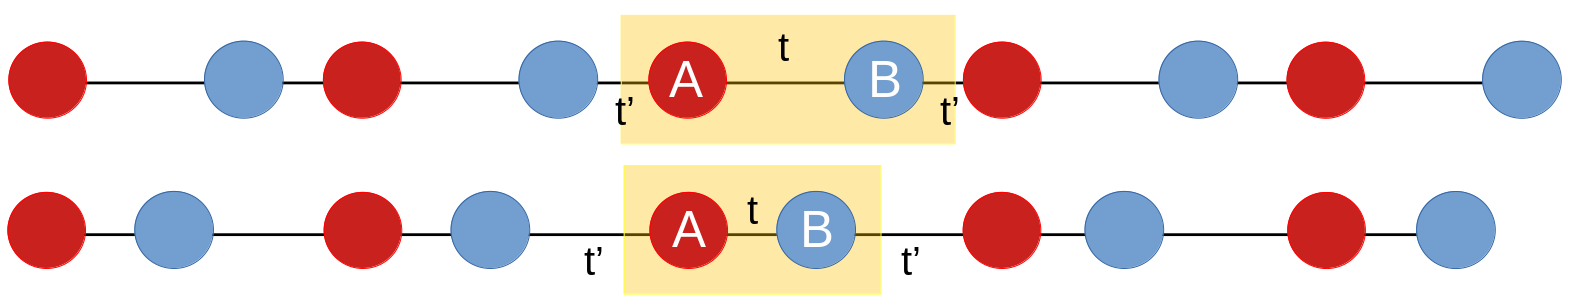
\includegraphics[width=\linewidth]{media/ssh-model.png}
	\caption[Schematic of the SSH model.]{Schematic of the SSH model. The unit cell is enclosed in yellow, where sites A and B and the intracell (intercell) coupling $t$ ($t'$) are distinguished. Two different configurations are shown. \label{fig:ssh-model}}
\end{figure}
Under periodic boundary conditions (Born–von Karman), it is possible to diagonalize the Hamiltonian in the Bloch basis with $a_n = \frac{1}{\sqrt{N}}\sum_k a_k e^{iknd}$, $b_n = \frac{1}{\sqrt{N}}\sum_k b_k e^{iknd}$ as follows:
\begin{align*}
	H &= \frac{1}{N}\sum_n \sum_{k k'} \left[\left(t + t' e^{ikd}\right) a_k b_{k'}^* e^{i(k-k')nd}  + \left(t  + t' e^{-ikd}\right) a_k^* b_{k'} e^{-i(k-k')nd} \right]
	\\
	&=  \sum_k 
	\begin{pmatrix}
		a_k^* & b_k^*		
	\end{pmatrix}
	\underbrace{
	\begin{pmatrix}
		0 & t+ t'e^{-ikd}
		\\
		t+ t'e^{ikd} & 0
	\end{pmatrix}}_{\hat{H}(k)}
	\begin{pmatrix}
		a_k
		\\
		b_k		
	\end{pmatrix},
\end{align*}
where it has been used that $$\frac{1}{N}\sum_n e^{i(k-k')nd} = \left\{\begin{matrix} \frac{N}{N}=1, &\text{ if } k = k'
\\ \frac{1}{N}\frac{1-\cancelto{1}{e^{i(k-k')Nd}}}{1-e^{i(k-k')d}}e^{i(k-k')d}=0, &\text{ if } k\neq k'
\end{matrix}\right. =\delta_{kk'},$$ since $k, k' \in  \left\{\frac{2\pi l}{Nd}, l=0,\pm 1, \dots , \pm \frac{N}{2}\right\}$ belong to the 1D reciprocal lattice. The spectrum of $\hat{H}(k)$ is $\lambda_k = \pm\sqrt{t^2+t'^2+2tt'\cos(kd)}$, which would seem to indicate that the system is symmetric between $t$ y $t'$. However, the picture is not complete without the eigenvectors of $\hat{H}(k)$, $\textbf{v}_\pm =\frac{1}{\sqrt{2}} \begin{pmatrix} \pm e^{-i\phi(k)} \\  1 \end{pmatrix}$, with $\phi(k)=\tan^{-1}\left(\frac{t'\sin(kd)}{t+t'\cos(kd)}\right)$. If the vector $\textbf{d}(k) \equiv \begin{pmatrix}t+t'\cos(kd) \\ t'\sin(kd) \\ 0 \end{pmatrix}$ is defined, it is possible to write the Hamiltonian $\hat{H}(k)$ in terms of the Pauli matrices as $\hat{H}(k) = \textbf{d} \cdot \bm{\sigma} = d_x\sigma_x + d_y\sigma_y$. This vector $\textbf{d}(k)$ is a vectorial representation of the $2\times2$ bulk Hamiltonian in momentum space. The phase $\phi(k)$ is related to the angle formed by the projection of the vector $\textbf{d}(k)$ onto the $xy$ plane,  $\phi(k)=\tan^{-1}\left( \frac{d_y}{d_x} \right)$. In particular, when $\delta \equiv t/t' < 1$, the vector $\textbf{d}(k)$ encloses the origin once, while for $\delta > 1$ it does not enclose the origin, as seen in Figure \ref{fig:ssh-topo}. Formally, the Zak phases, $\mathcal{Z}_\pm$, associated with the bulk eigenstates (a region sufficiently far from the edges) change depending on the value of $\delta$.  By definition \citep{zak_berry}, \begin{align*}
\mathcal{Z}_\pm &= i \oint \textbf{v}_\pm^\dagger \frac{d \textbf{v}_\pm}{dk}  dk  = -\frac{1}{2} \int_{-\frac{\pi}{d}}^{{\frac{\pi}{d}}}  \frac{d \phi(k)}{d k} dk = -\frac{d}{2}\int_{-\frac{\pi}{d}}^{{\frac{\pi}{d}}} \frac{1+\delta\cos(kd)}{\delta^2+1+2\delta\cos(kd)} dk = -\frac{\pi}{2} \left(1 + \frac{1-\delta^2}{\left|1-\delta^2\right|} \right) \ .
\end{align*}
That is,
\begin{align*}
\mathcal{Z}_\pm &= \left\{\begin{matrix}
-\pi, &\text{ if } |\delta| < 1
\\
0, &\text{ if } |\delta| > 1
\end{matrix}\right. \ .
\end{align*}
The change in the Zak phase as the parameter $\delta$ varies is known as a \textit{topological transition} since it is not possible to smoothly transition from one regime to the other. This has implications for the system with open boundary conditions (Dirichlet) due to the \textit{bulk-boundary correspondence} \cite{topobulk}. Specifically, as illustrated in Figure \ref{fig:ssh-open}, the topology of the Hamiltonian $\hat{H}(k)$ induces the appearance of zero-energy edge states when open boundary conditions are imposed.

The Hamiltonian of the SSH model exhibits various symmetries: time-reversal, inversion, particle-hole, translational, and chiral. The latter is particularly relevant, as the edge states of the SSH model are \textit{topologically protected} against any disorder that respects chiral symmetry \cite{ssh-course}. The chiral operator in question is the Pauli matrix $\sigma_z$, since 
\begin{align*}
	\left\{\hat{H}(k), \sigma_z \right\} = \left\{d_x \sigma_x + d_y\sigma_y , \sigma_z \right\} = d_x \cancelto{0}{\left\{\sigma_x, \sigma_z \right\}} + d_y \cancelto{0}{\{\sigma_y, \sigma_z\}} = 0 \ .
\end{align*}
\begin{figure}[h]
	\centering
	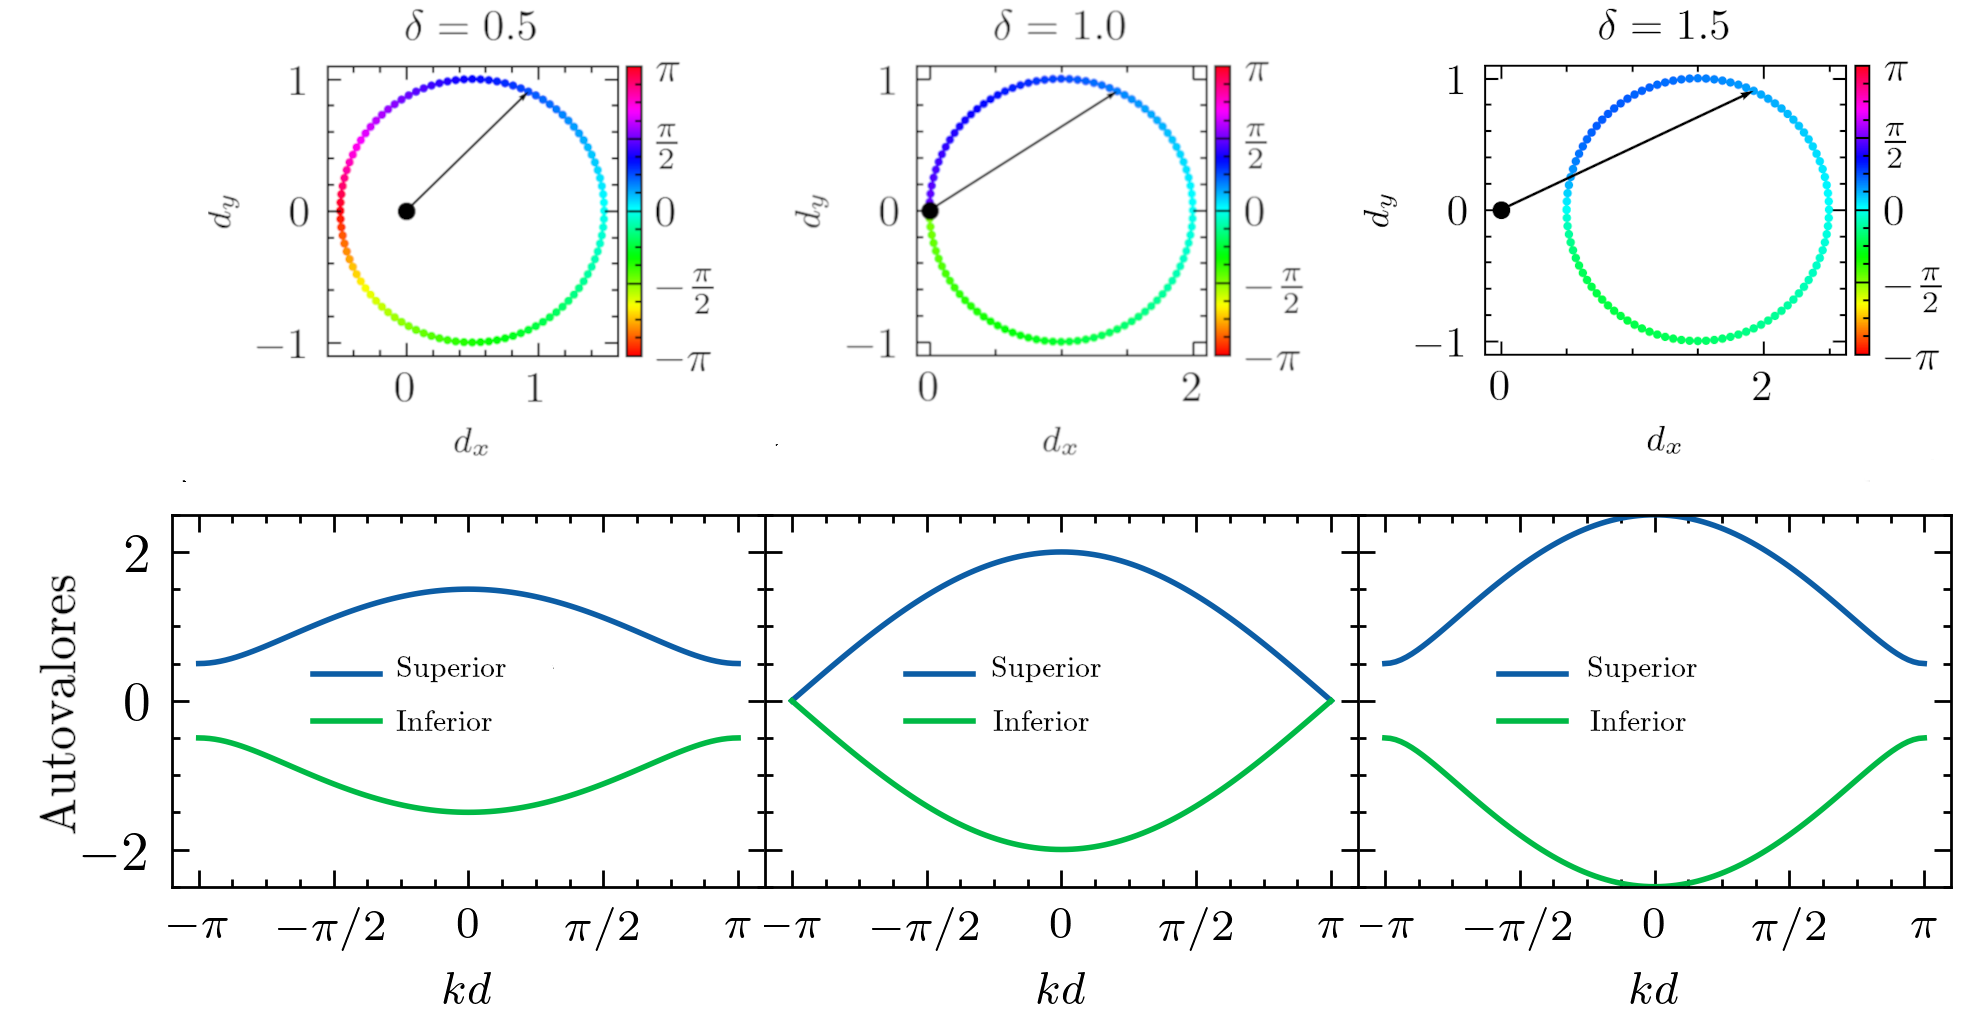
\includegraphics[width=\linewidth]{media/ssh-winding}
\caption[Topology of the SSH lattice.]{Topology of the SSH lattice. Top: Vectors $\textbf{d}$(k) and their phase. For $\delta < 1$ ($\delta > 1$), the origin is (not) enclosed. Bottom: Bands as a function of quasimomentum $k$ in the first Brillouin zone for $\delta < 1$, $\delta = 1$ and $\delta > 1$. Here $t'=1$ is fixed and $\delta'$ is varied for a number $N=100$  of unit cells.
	\label{fig:ssh-topo}}
\end{figure} \begin{figure}[h]
\centering	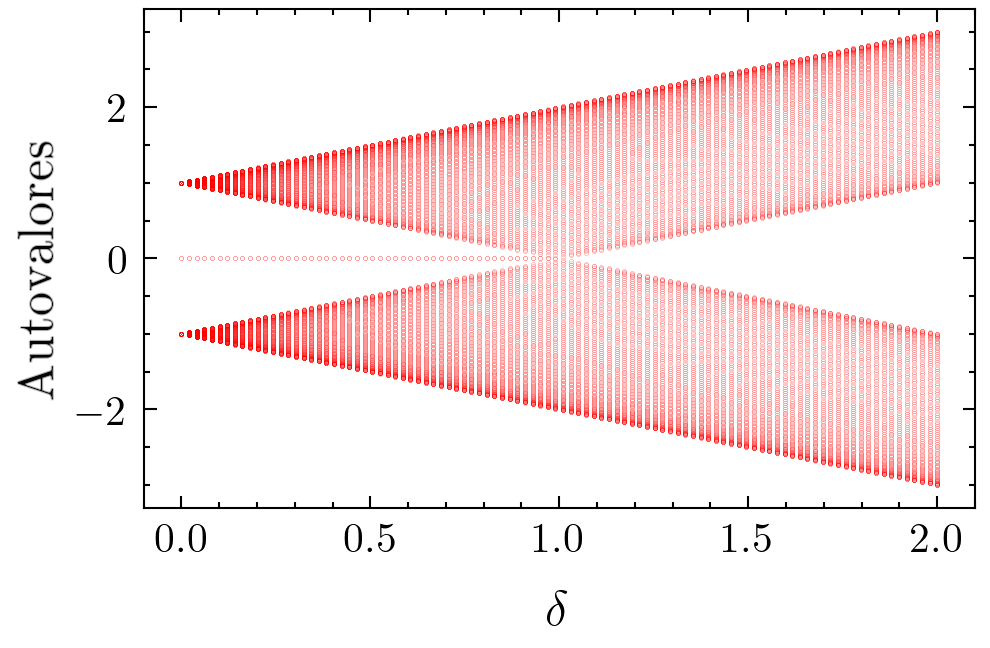
\includegraphics[width=0.7\linewidth]{media/ssh-open}
	\caption[Spectrum of the finite SSH lattice.]{Spectrum of the finite SSH lattice. The emergence of zero-energy edge states for $\delta < 1$ is observed. Open boundary conditions as a function of the parameter $\delta=t/t'$, with fixed $t'=1$  and a number $N=100$ of unit cells.
		\label{fig:ssh-open}}
\end{figure} 

\chapter{Numerical Methods \label{cap:num}}
In this chapter, the fundamental numerical methods used to model the electromagnetic behavior in the photonic systems studied in this thesis are presented. Since most of these systems lack exact analytical solutions, especially in the absence of exploitable symmetries, numerical approaches are essential to obtain approximations with controlled precision.

The theoretical starting point is provided by the vectorial Helmholtz equations for the electric and magnetic fields, expressed in Eqs. (\ref{eqn:helmholz}) and (\ref{eqn:helmholzH}), which describe the propagation of electromagnetic waves in dielectric media. By applying the weak guidance approximation, the coupled terms on the right-hand side of both equations can be neglected. This crucial simplification eliminates cross effects between the transverse and longitudinal components of the fields, effectively decoupling the equations and reducing the complex vector problem to a set of independent scalar Helmholtz equations, which are numerically manageable. This scalar formulation is the foundation upon which the computational methods described below are implemented.
\begin{equation}
\left[\nabla^2 + k_0^2 n^2(\textbf{r})\right]\Psi(\textbf{r}) = 0 \ , \label{eqn:helmholtznum}
\end{equation}
where equation (\ref{eqn:helmholznum}) serves not only as a theoretical framework but also as the foundation for the algorithms developed in the following chapters. Its versatility allows for the adaptation of different numerical schemes according to the symmetries of the problem, as will be detailed in the subsequent sections.
\section{Eigenmode Expansion \label{cap:eme}}
This numerical method, developed and implemented during the student's Master's research, is useful when the photonic systems under study are invariantThe solutions to equation (\ref{eqn:helmholtznum}) can be expanded in plane waves with transverse profiles: $\Psi(\textbf{r}) = \Psi(x,y) \exp({i\beta z})$. With this, each transverse mode νν must satisfy the following equation to be solved numerically:
\begin{equation}
	\left[\nabla_\perp^2 + k_0^2 n^2(x,y)\right]\Psi_\nu(x,y) = \beta_\nu^2\Psi_\nu(x,y) \ , \quad\text{ con } \nabla_\perp^2 \equiv \frac{\partial^2}{\partial x^2} + \frac{\partial^2}{\partial y^2} \ .
	\label{eqn:eme}
\end{equation}
And the total propagated field is a linear combination of the modes $\Psi_\nu$: 
\begin{equation}
	\Psi(\textbf{r}) = \sum_\nu a_\nu \Psi_\nu(x,y) e^{i\beta_\nu z} \ , \quad\text{ con } a_\nu \propto \Psi_\nu(x,y) \cdot \Psi(x, y, z=0) \ . \label{eqn:emedin}
\end{equation}
Instead of directly integrating the eigenvalue equation (\ref{eqn:eme}), the strategy will be to discretize space and approximate the transverse Laplacian operator $\nabla_\perp^2$ as a matrix, since $$\frac{\partial^2 \Psi(x,y)}{\partial x^2} \sim \frac{\Psi[i+1,j]-2\Psi[i,j]+\Psi[i-1,j]}{\Delta x ^2}  \ .
$$
$\nabla^2_\perp \sim \hat{D}_{xx} \otimes I_y + I_x \otimes \hat{D}_{yy}$
The matrix is null in off-diagonal positions beyond a certain spacing (\textit{sparse-like}), so it is possible to optimize the computation process by using the Python library \href{https://docs.scipy.org/doc/scipy/reference/sparse.linalg.html}{\color{magenta}\texttt{scipy.sparse.linalg}}, specifically designed for sparse matrix linear algebra. Appendix \ref{sec:codigohelmholtz} contains an implementation of this algorithm in Python under the \href{https://www.gnu.org/licenses/gpl-3.0.html}{\color{magenta}GNU GPL v3 license}.

In Figure \ref{fig:emenumerror}, the numerical method is validated by comparison with the analytical solutions obtained in Subsection \ref{cap:solslabTETM}. The complexity of the problem is on the order of $O(N^2)$ due to the construction of the $N\times N$ matrices, which is reflected in the dependence of the execution time on the step size $\Delta x \equiv \frac{L}{N-1}$.


\begin{figure}[H]
	\centering
	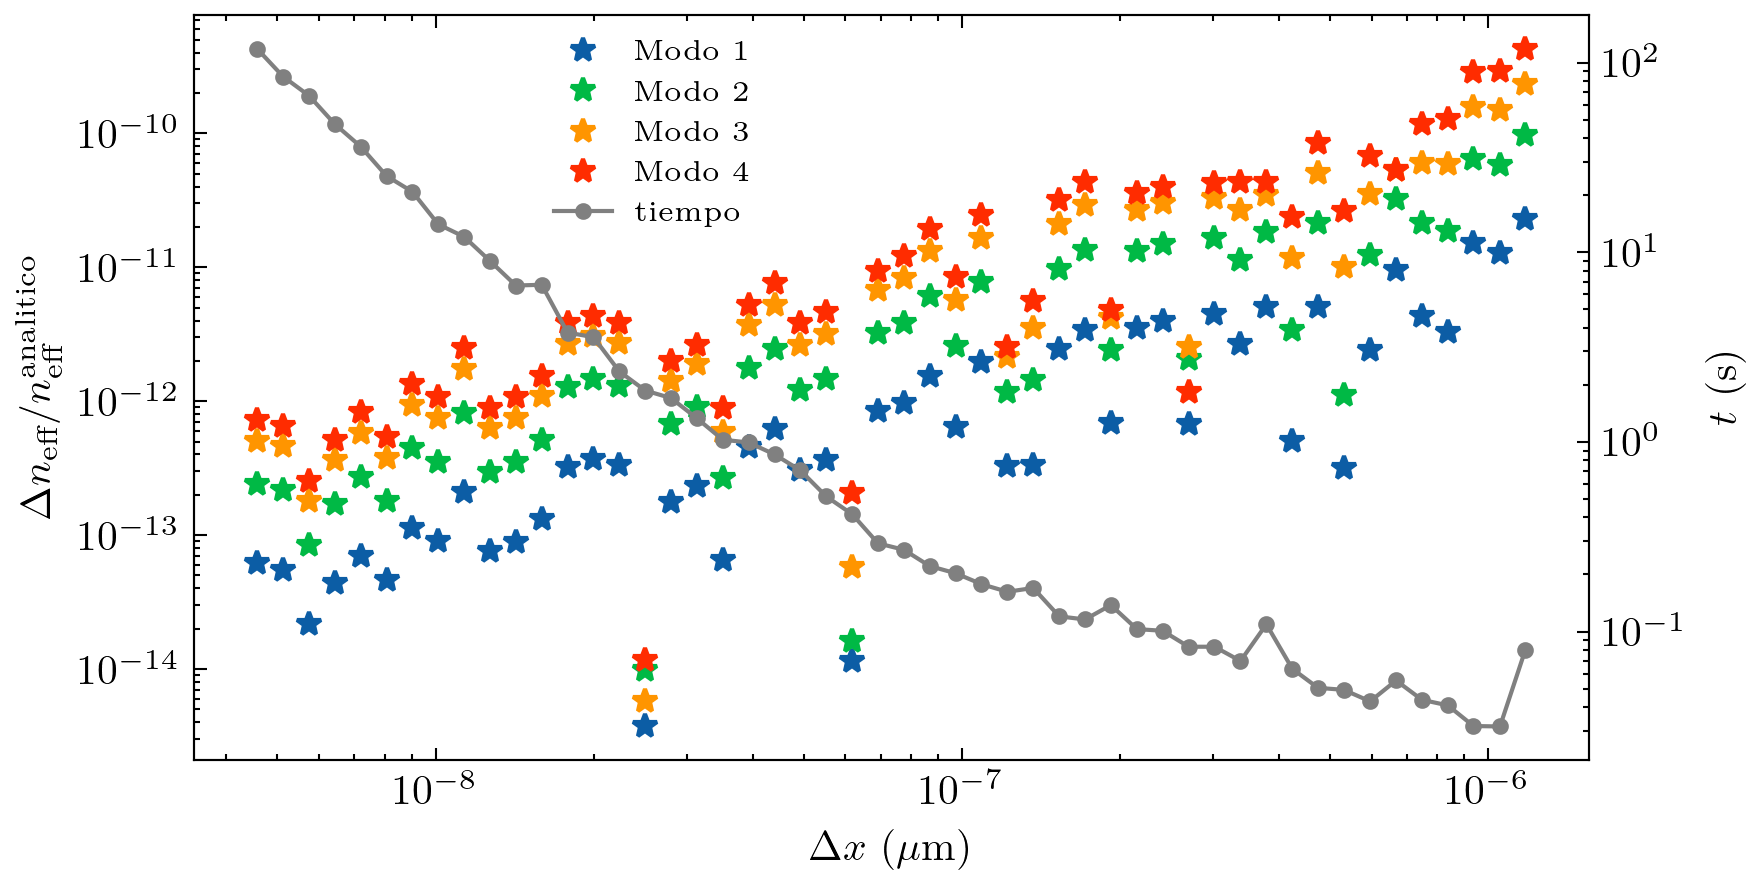
\includegraphics[width=\linewidth]{media/numerical_slab}
	\caption[Relative error and execution time.]{Relative error and execution time of the numerical solutions to equation (\ref{eqn:eme}) compared to the analytical solutions, as a function of the step size $\Delta x$. \label{fig:emenumerror}}
\end{figure}
\section{Beam Propagation Method}
Another way to approach the numerical integration of equation (\ref{eqn:helmholtznum}) involves separating the field into its slow envelope and a rapidly oscillating phase, considering that in the visible range the order of magnitude is $k_0 \sim 10 ^{5} \text{ cm}^{-1}$: $\Psi(\textbf{r}) = \phi(x,y,z)\exp(ik_0 n_0 z)$. After substituting into equation (\ref{eqn:helmholtznum}), the optical Schrödinger equation is obtained \citep{paraxialschrodinger}:
\begin{equation}
	-2ik_0 n_0\frac{\partial }{\partial z}\phi(x,y, z) =  \left[\nabla_\perp^2 + k_0^2 (n^2(\textbf{r})-n_0^2)\right]\phi(x,y, z) \ , \label{eqn:bpmescalar}
\end{equation} 
where the paraxial approximation $\left| \frac{\partial^2 \phi}{\partial z^2} \right| \ll 2 k_0 n_0\left| \frac{\partial \phi}{\partial z} \right|$has been used. Algorithms that solve equation (\ref{eqn:bpmescalar}) are known as scalar Beam Propagation Methods (BPM), widely used in this research area \cite{bics, interorbital, OAMCaging, vortex, bpm}. Outside the weak guidance approximation, cross-polarization effects become more relevant, and a vectorial description of the problem is necessary.
\subsection{Implementation via Fourier Transform (FFTBPM)}
Equation (\ref{eqn:bpmescalar}) can be written in terms of linear differential operators as \citep{bpm}:
\begin{equation}
	\frac{\partial \phi}{\partial z}  = \left(\hat{A} + \hat{B}\right)\phi, \text{ con } \hat{A} \equiv i\frac{\nabla^2_\perp}{2k_0n_0}\text{ y } \hat{B} \equiv i\frac{k_0}{2n_0}\left[n^2(\textbf{r})-n_0^2\right] \ . \label{eqn:bpmop}
\end{equation}
The formal solution to equation (\ref{eqn:bpmop}) is $\phi(\textbf{r}) = \exp\left[\left(\hat{A} + \hat{B}\right)(z-z_0)\right]\phi(x, y, z_0)$. It is convenient to work with the operator \( \hat{A} \) in Fourier space and the operator \( \hat{B} \) in real space. This is because \( \hat{A} \) contains spatial derivatives—in particular, the transverse Laplacian operator \( \nabla^2_\perp \)— which become simple multiplications upon applying the Fourier transform. Thus, the operation \( \hat{A} \phi \) becomes computationally efficient when transformed into the wavevector domain \( \textbf{k}_\perp \), where it acts as a diagonal operator. On the other hand, \( \hat{B} \) depends on the spatial profile of the refractive index \( n(\textbf{r}) \), which is defined locally in real space. Evaluating this term in Fourier space would involve a convolution, which is unnecessarily costly and less intuitive. For this reason, it is kept in real space.

Since $\hat{A}$ and $\hat{B}$ do not commute in general, the exponential operator can be expanded to order $O(\Delta z ^3)$ as $\exp\left[\left(\hat{A} + \hat{B}\right)\Delta z \right] \approx \exp\left(\frac{\hat{A}\Delta z}{2} \right)\exp\left(\hat{B}\Delta z \right)\exp\left(\frac{\hat{A}\Delta z}{2} \right) + O(\Delta z ^3)$.

The algorithm implemented in Appendix \ref{sec:codeBPM} is as follows: \begin{enumerate}
	\item Start with a profile $\phi(x, y, z_0)$
\item Act in Fourier space by transforming the profile and multiplying by the phase associated with $\hat{A}$: $\exp\left(\frac{ik^2\Delta z}{4k_0 n_0}\right)\mathcal{F}(\phi(z_0))$, where $k=\sqrt{k_x^2 + k_y^2}$ are the Fourier frequencies.
\item Apply the inverse Fourier transform and multiply by the phase associated with $\hat{B}$: 

$\exp\left[\frac{i\Delta z k_0^2(n^2-n_0^2)}{2 k_0n_0}\right]\mathcal{F}^{-1}\left(\exp\left(\frac{ik^2 \Delta z}{4k_0 n_0}\right)\mathcal{F}(\phi(z_0))\right)$
\item Return to Fourier space and multiply by the phase associated with $\hat{A}$:
 
$\exp\left(\frac{ik^2\Delta z}{4k_0 n_0}\right)\mathcal{F}\left\{\exp\left[\frac{ik_0^2(n^2-n_0^2)}{2 k_0n_0}\Delta z \right]\mathcal{F}^{-1}\left[\exp\left(\frac{ik^2\Delta z}{4k_0 n_0}\right)\mathcal{F}(\phi(z_0))\right]\right\}$
\item Return to real space, having advanced one step $\Delta z$:

$\phi(z_0+\Delta z)=\mathcal{F}^{-1}\left\{\exp\left(\frac{ik^2\Delta z}{4k_0 n_0}\right)\mathcal{F}\left\{\exp\left[\frac{i k_0^2(n^2-n_0^2)}{2 k_0n_0}\Delta z\right]\mathcal{F}^{-1}\left[\exp\left(\frac{ik^2\Delta z}{4k_0 n_0}\right)\mathcal{F}(\phi(z_0))\right]\right\} \right\}$

\item Iterate until the desired propagation distance zz is reached.
\end{enumerate} Figure \ref{fig:num-exp-comp} compares experimental results with numerical simulations obtained via BPM. The normalized intensity profiles show remarkable qualitative agreement, particularly in the spatial distribution of the main lobes.

\begin{figure}[H]
	\centering
	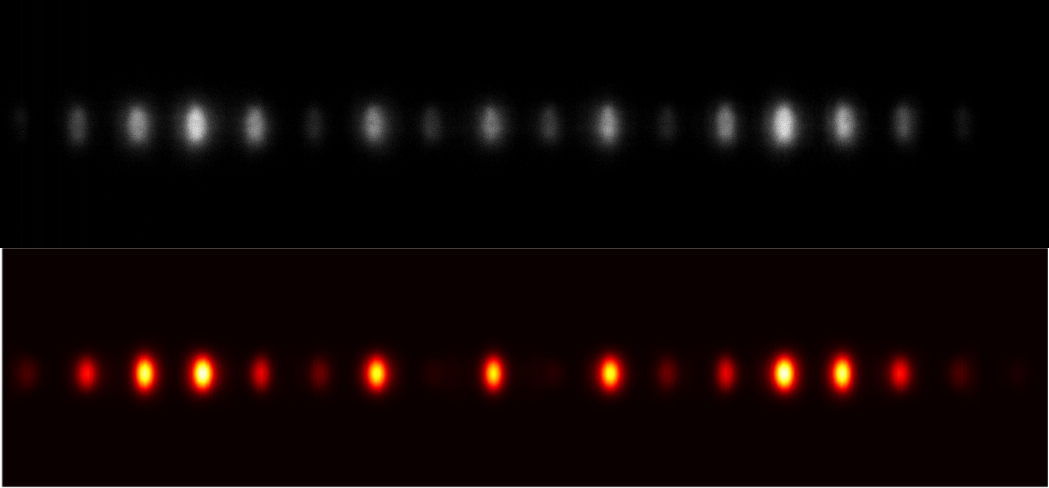
\includegraphics[width=\linewidth]{media/num_exp_comparison.png}
	\caption[Excitation of the central site of a one-dimensional lattice.]{Excitation of the central site of a one-dimensional lattice.
		\textbf{Top:} Experimental measurement at $\lambda$ = 730 nm.
textbf{Bottom:} Numerical simulation performed with BPM.
\label{fig:num-exp-comp}} \end{figure} This level of qualitative agreement validates the weak guidance approximation used in equation (\ref{eqn:helmholtznum}), as well as the paraxial approximation, and reinforces the reliability of the numerical method for designing photonic devices with analogous geometries.

\section{Comments on Coupled-Mode Theory \label{cap:CMT}}
The numerical simulation of equations (\ref{eqn:non-ortho-CMT-eqs}) represents the most compact formulation possible, since the coupling matrix $\hat{C} \equiv \hat{P}^{-1}\hat{H}$ encodes all the properties of the network to be studied in a semi-empirical manner. In this sense, the diagonalization of $\hat{C}$ constitutes a valuable numerical tool for analyzing the behavior of photonic networks under variations of parameters such as dimerization (defined as the ratio between two coupling constants) or detuning (the difference between the propagation constants of distinct modes).

Furthermore, this approach allows for the exploration of even "non-physical" systems, thanks to the degrees of freedom available in the elements of $\hat{C}$: for example, cases where second-neighbor coupling is greater than first-neighbor coupling, or systems with complex couplings.

In the weak guidance approximation, the longitudinal components of the electric field can be neglected:
\[ \nabla \cdot (n^2 \textbf{E}) \overset{\nabla n^2 \sim 0}{\sim} n^2 \nabla \cdot \textbf{E} = 0 \ ,\]
where the order of magnitude of the longitudinal field component is $|E_z| \sim |\nabla_\perp \cdot \textbf{E}_\perp|/\beta$. Thus, the studied modes are quasi-transverse, and the matrix $\hat{P}$ reduces to:
\begin{equation}
    P_{ij} \sim \frac{k_z^i + k_z^j}{4\omega\mu_0} \iint \left(\textbf{e}_i^\perp\right)^* \cdot \textbf{e}_j^\perp dxdy \ .
    \label{eqn:CMTnum}
\end{equation}
Equation (\ref{eqn:CMTnum}), which quantifies the overlap between modes, along with equation (\ref{eqn:hij}) describing the matrix elements of the Hamiltonian operator, constitute fundamental tools for the comparative analysis between the Eigenmode Expansion (EME) method and Coupled-Mode Theory (CMT). This comparison is performed through a systematic study of the eigenvalue spectrum of the coupling matrix $\hat{C}$, which contains essential information about the effective propagation constants of the system.

Figure \ref{fig:EMECMT} presents a quantitative analysis of this comparison, showing the evolution of the eigenvalues for a dielectric photonic coupler as a function of the separation distance between waveguides. It is observed that both methods converge asymptotically for distances greater than $d > 20\,\mu$m, where the weak field approximation of CMT holds. However, in the strong coupling regime ($d < 13\,\mu$m), discrepancies begin to become noticeable.

Beyond the spectral analysis, the validity of the computed eigenstates can be indirectly verified through equation (\ref{eqn:emedin}), which relates the field evolution to the projection onto the system's eigenmodes, and by qualitatively comparing the dynamic profiles obtained with the experimental and numerical results shown in Figure \ref{fig:num-exp-comp}. This analysis (see Figure \ref{fig:1darraycmt}) allows establishing the applicability limits of each numerical method: while EME provides accurate results across the entire parameter range at the cost of higher computational complexity, CMT offers an efficient alternative for weakly coupled systems where the approximation of localized modes remains valid: separation distances $d \gtrapprox$ 15 $\mu$m.
\begin{figure}[h]
    \centering
    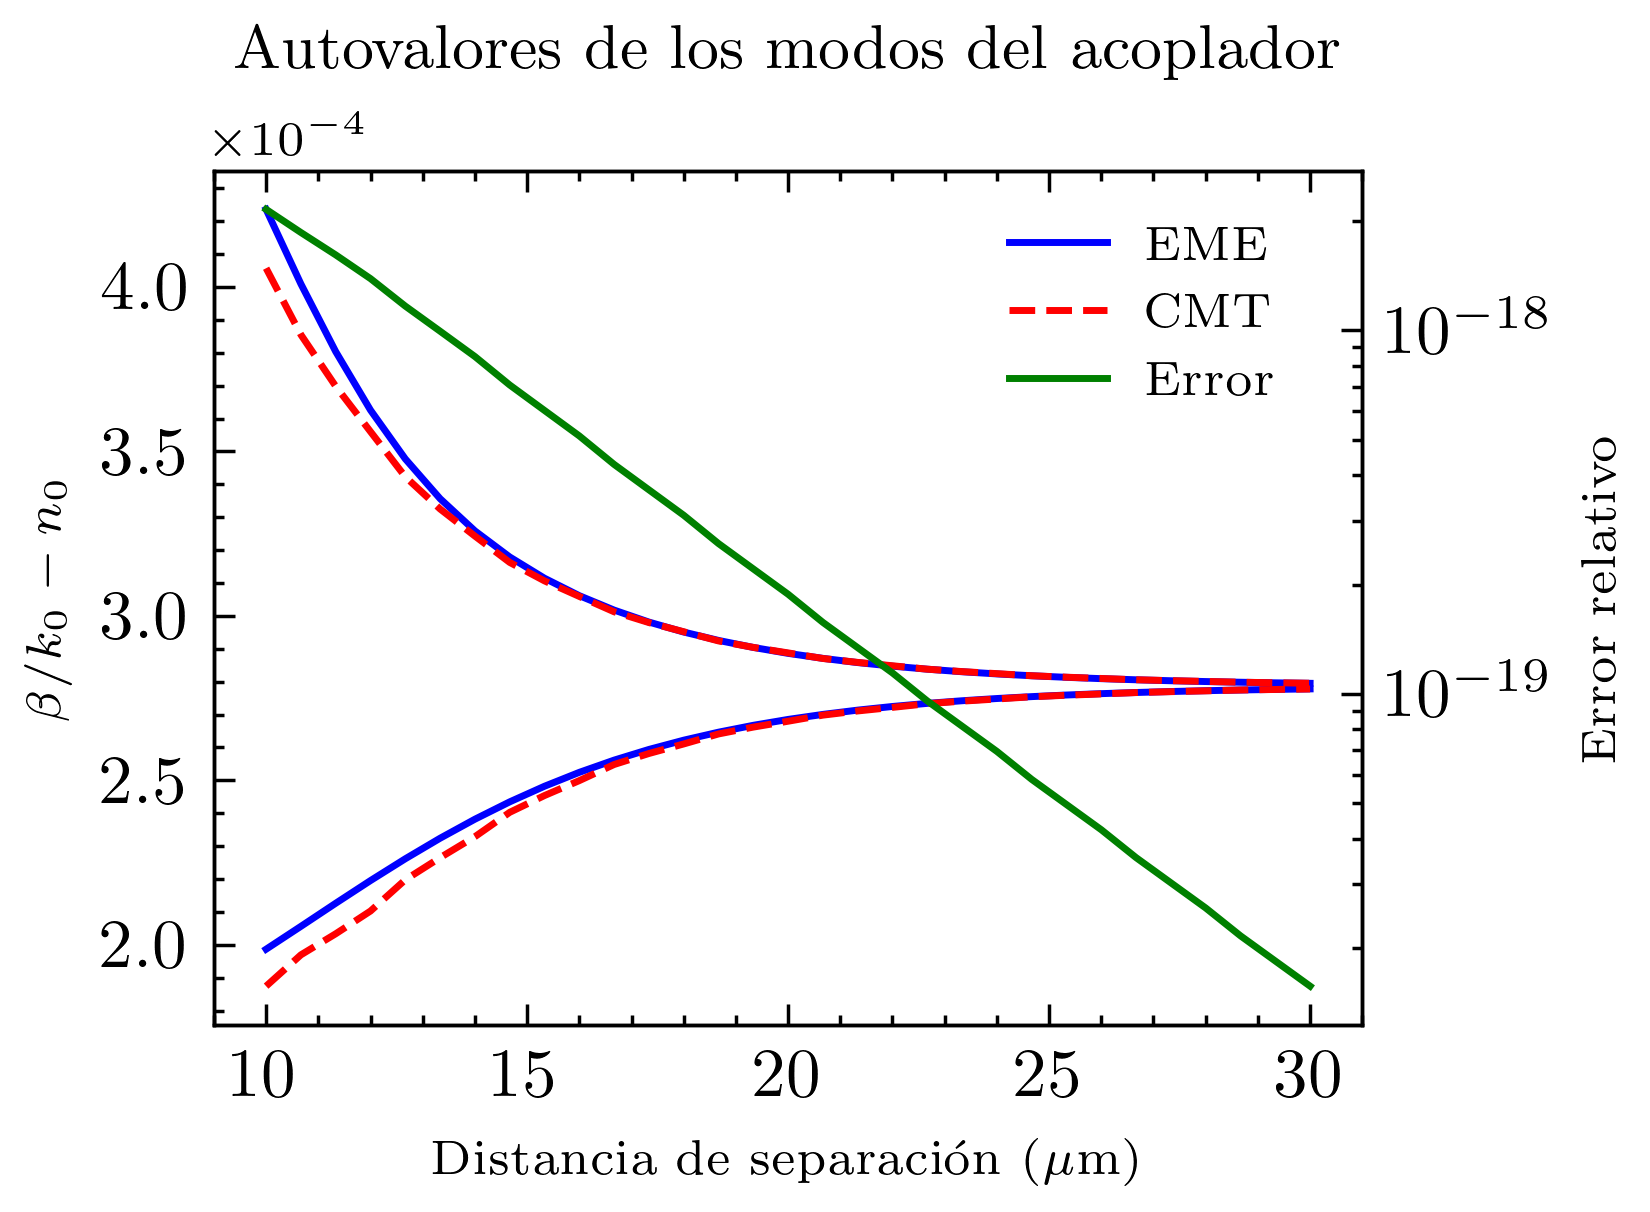
\includegraphics[width=0.8\linewidth]{codigo/dimol/coupler.png}
    \caption[Comparison between EME and CMT.]{Comparison of the eigenvalues obtained with the Eigenmode Expansion (EME) method and with Coupled-Mode Theory (CMT). Greater divergence is observed when the distance between waveguides is small. Parameters used: $n_0=1.48$, $\Delta n = 4\times10^{-4}$, $\lambda = 730$ nm y $a = 3\,\mu$m.}
    \label{fig:EMECMT}
\end{figure}
\begin{figure}[h]
	\centering
	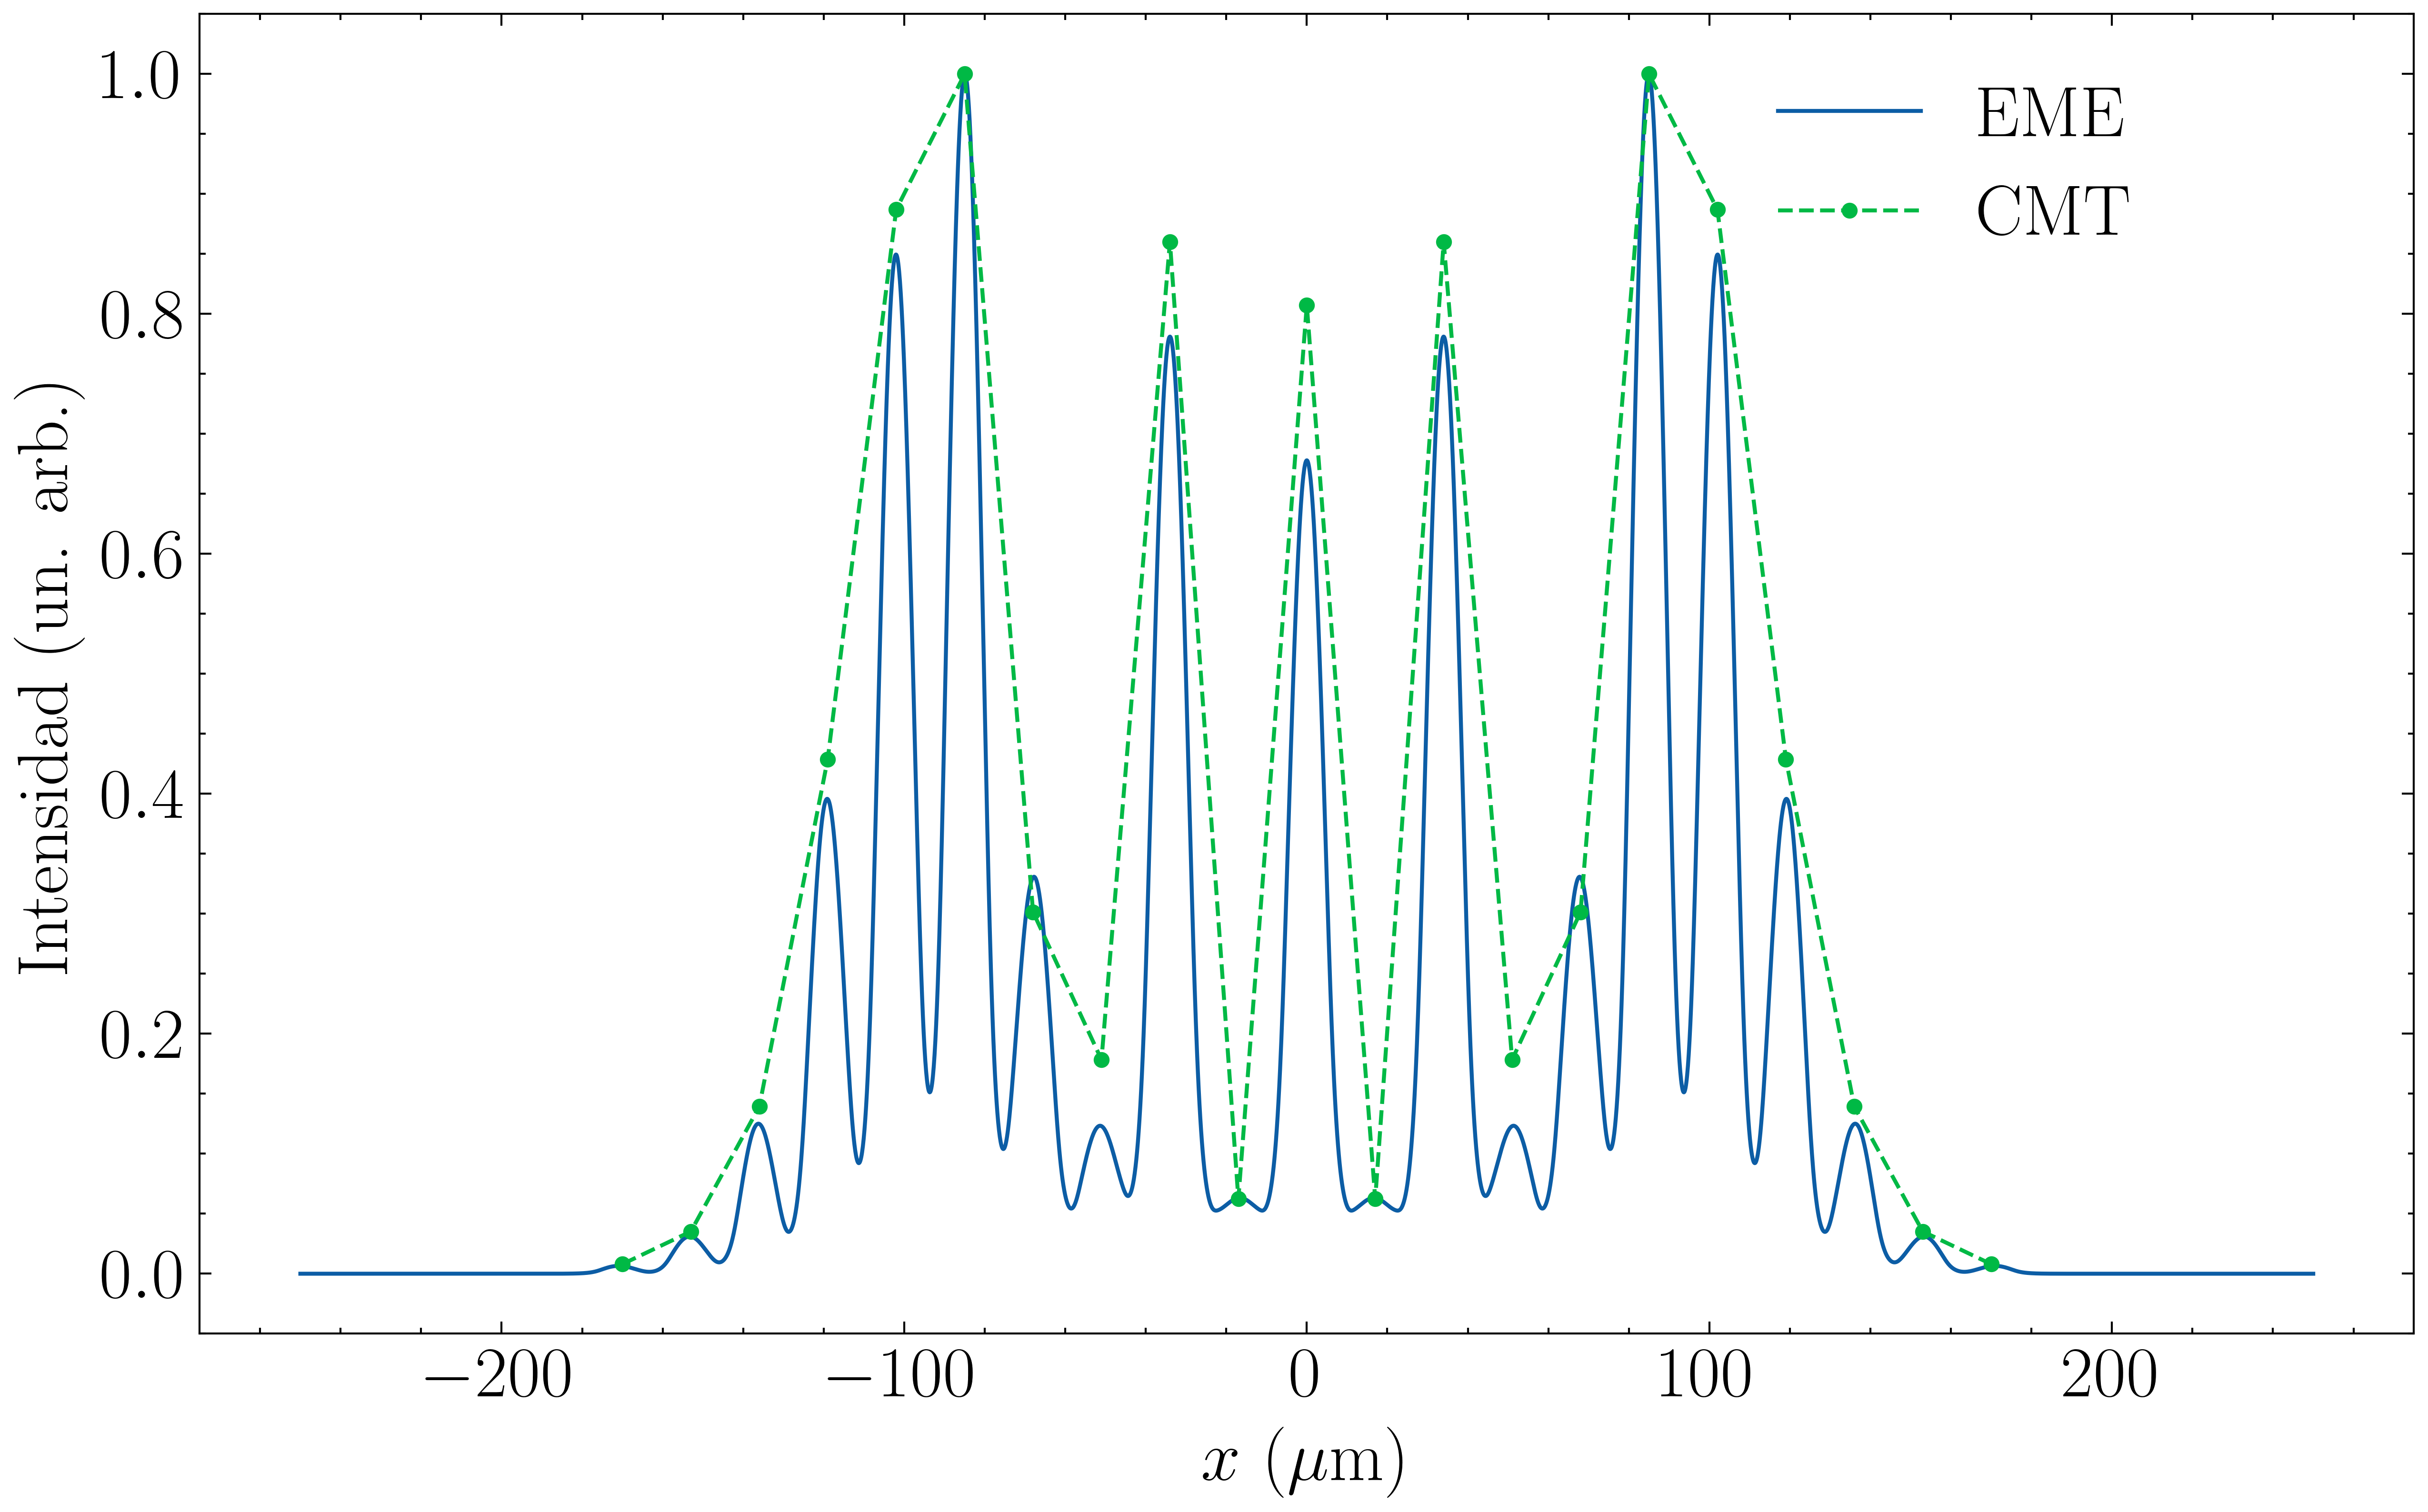
\includegraphics[width=0.8\linewidth]{codigo/1darraycmt/1darraycmt.png}
	\caption[Dynamics with EME and CMT.]{Dynamic profile of a one-dimensional array of 21 waveguides at a distance $d=17$ $\mu$m simulated with CMT and with EME. The results are similar to those in Figure \ref{fig:num-exp-comp}.}
	\label{fig:1darraycmt}
\end{figure}

\chapter{Experimental Methods \label{cap:exp}}

This chapter details the experimental procedures developed for the fabrication and characterization of photonic networks based on waveguides. The methodology encompasses three fundamental aspects: (1) direct writing of waveguides using a femtosecond laser, (2) optical excitation systems with a supercontinuum laser, and (3) advanced techniques for spatial light modulation to control initial conditions.


\section{Direct Writing of Waveguides \label{cap:fs}}

The fabrication of waveguides was carried out using the direct writing technique with a femtosecond laser: ultrashort pulses emitted from a Yb-doped fiber laser ATSEVA ANTAUS at 1030 nm, with a repetition rate of 500 kHz, are strongly focused into a borosilicate sample, producing slight and permanent changes in the local refractive index $\Delta n \sim 10^{-4}-10^{-3}$. This method, available and implemented by previous members of the Photonic Networks Group, allows for the creation of three-dimensional structures through computer-controlled movements of the Aerotech Nanopositioner XYZ platform \citep{femto_writing}.

\begin{figure}[H]
    \centering
    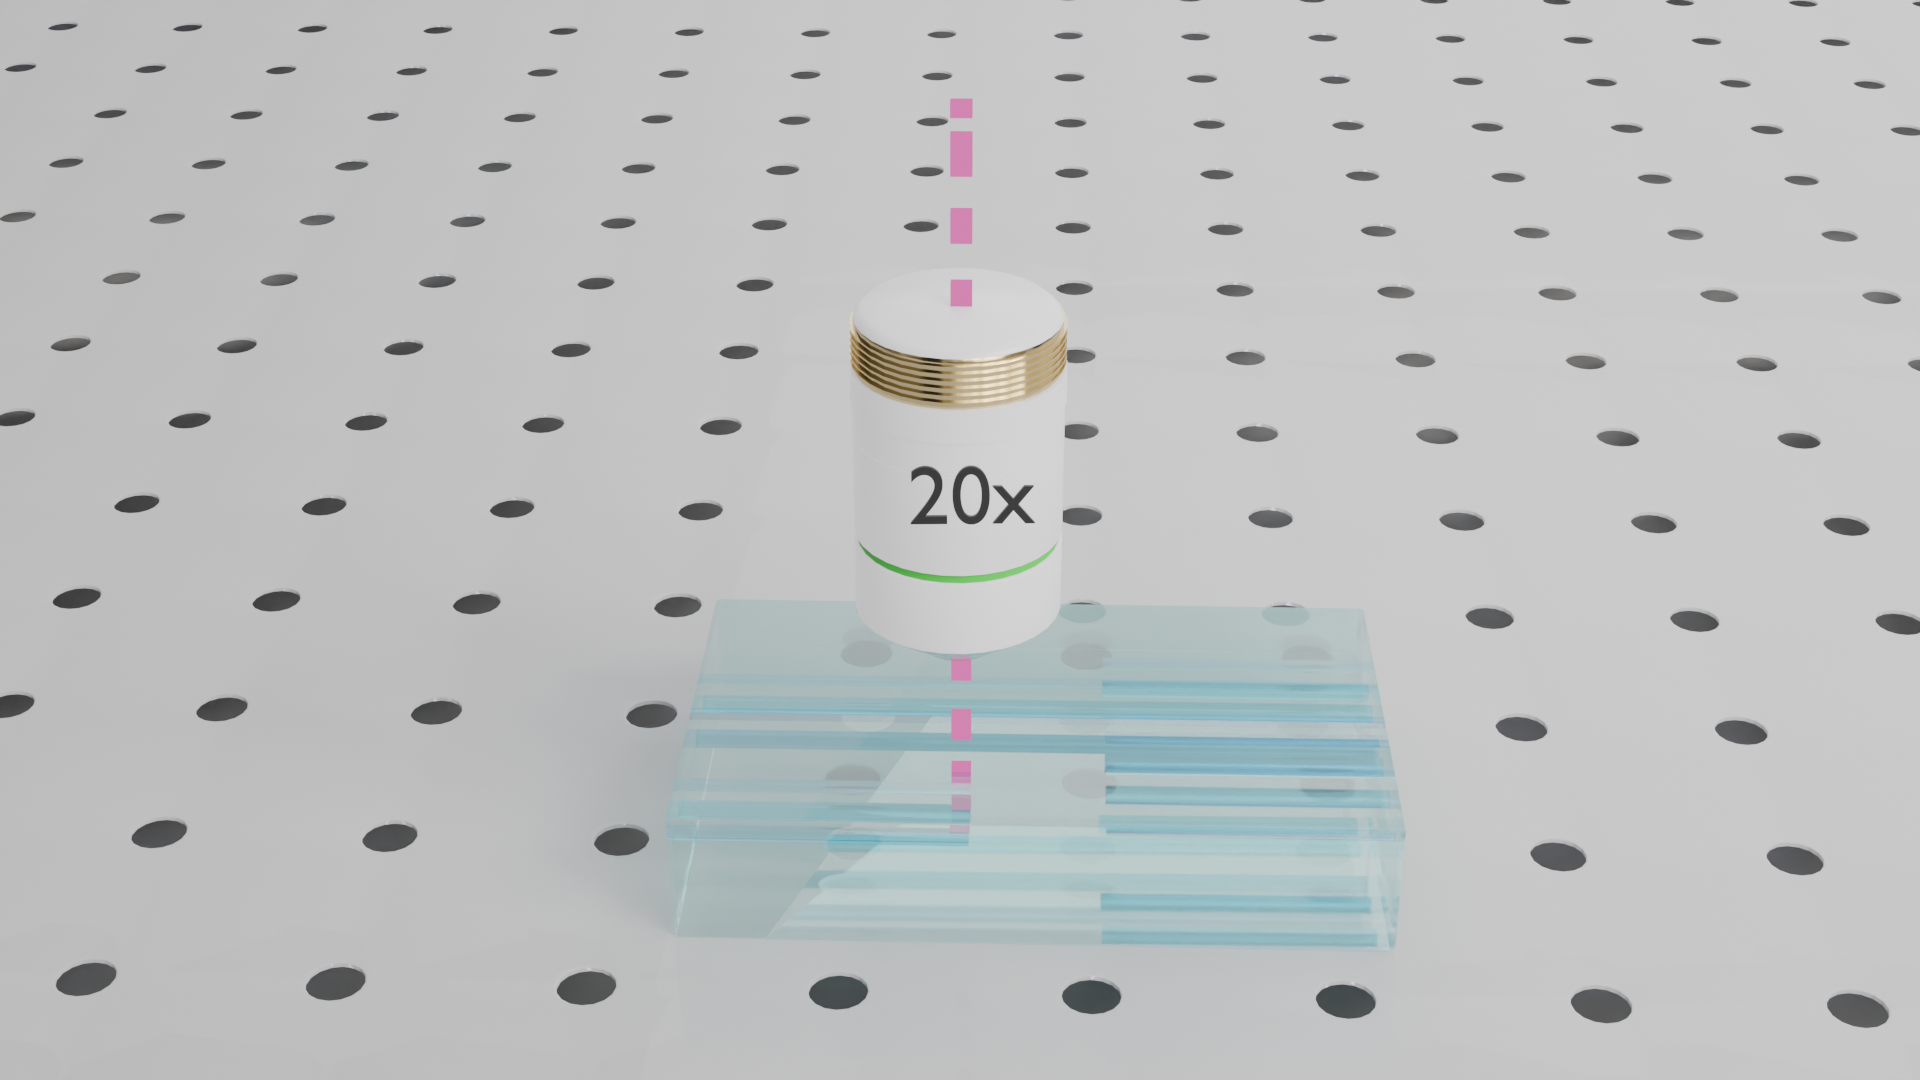
\includegraphics[width=0.5\linewidth, trim={18cm 4cm 15cm 6cm},clip]{media/fabrication1}
    \caption[Schematic of the waveguide writing technique.]{Schematic of the waveguide writing technique. The laser beam is focused using a microscope objective (20x) while the sample is moved along three axes via a computer-controlled platform.}
\end{figure}

The writing parameters that work for exciting modes in the visible spectrum are:
\begin{itemize}
	\item Pulse width: 215 fs.
	\item Repetition rate: 500 kHz.
	\item Writing speed: 0.1 - 20.0 mm/s.
	\item Measured arrival power: 70.0 - 150.0 mW.
\end{itemize}

\section{Supercontinuum Laser Excitation Setup \label{cap:wavelength}}

For optical characterization, an excitation system based on a broadband supercontinuum (SC) laser (470 nm - 2200 nm) was implemented. Specifically, the model is a YSL SC-5. The configuration allows selecting specific wavelengths through an acousto-optic modulator AOTF-PRO (430 nm - 1450 nm), with a spectral resolution of $\pm$5 nm and an output power of 1 mW per wavelength.

\begin{figure}[H]
    \centering
    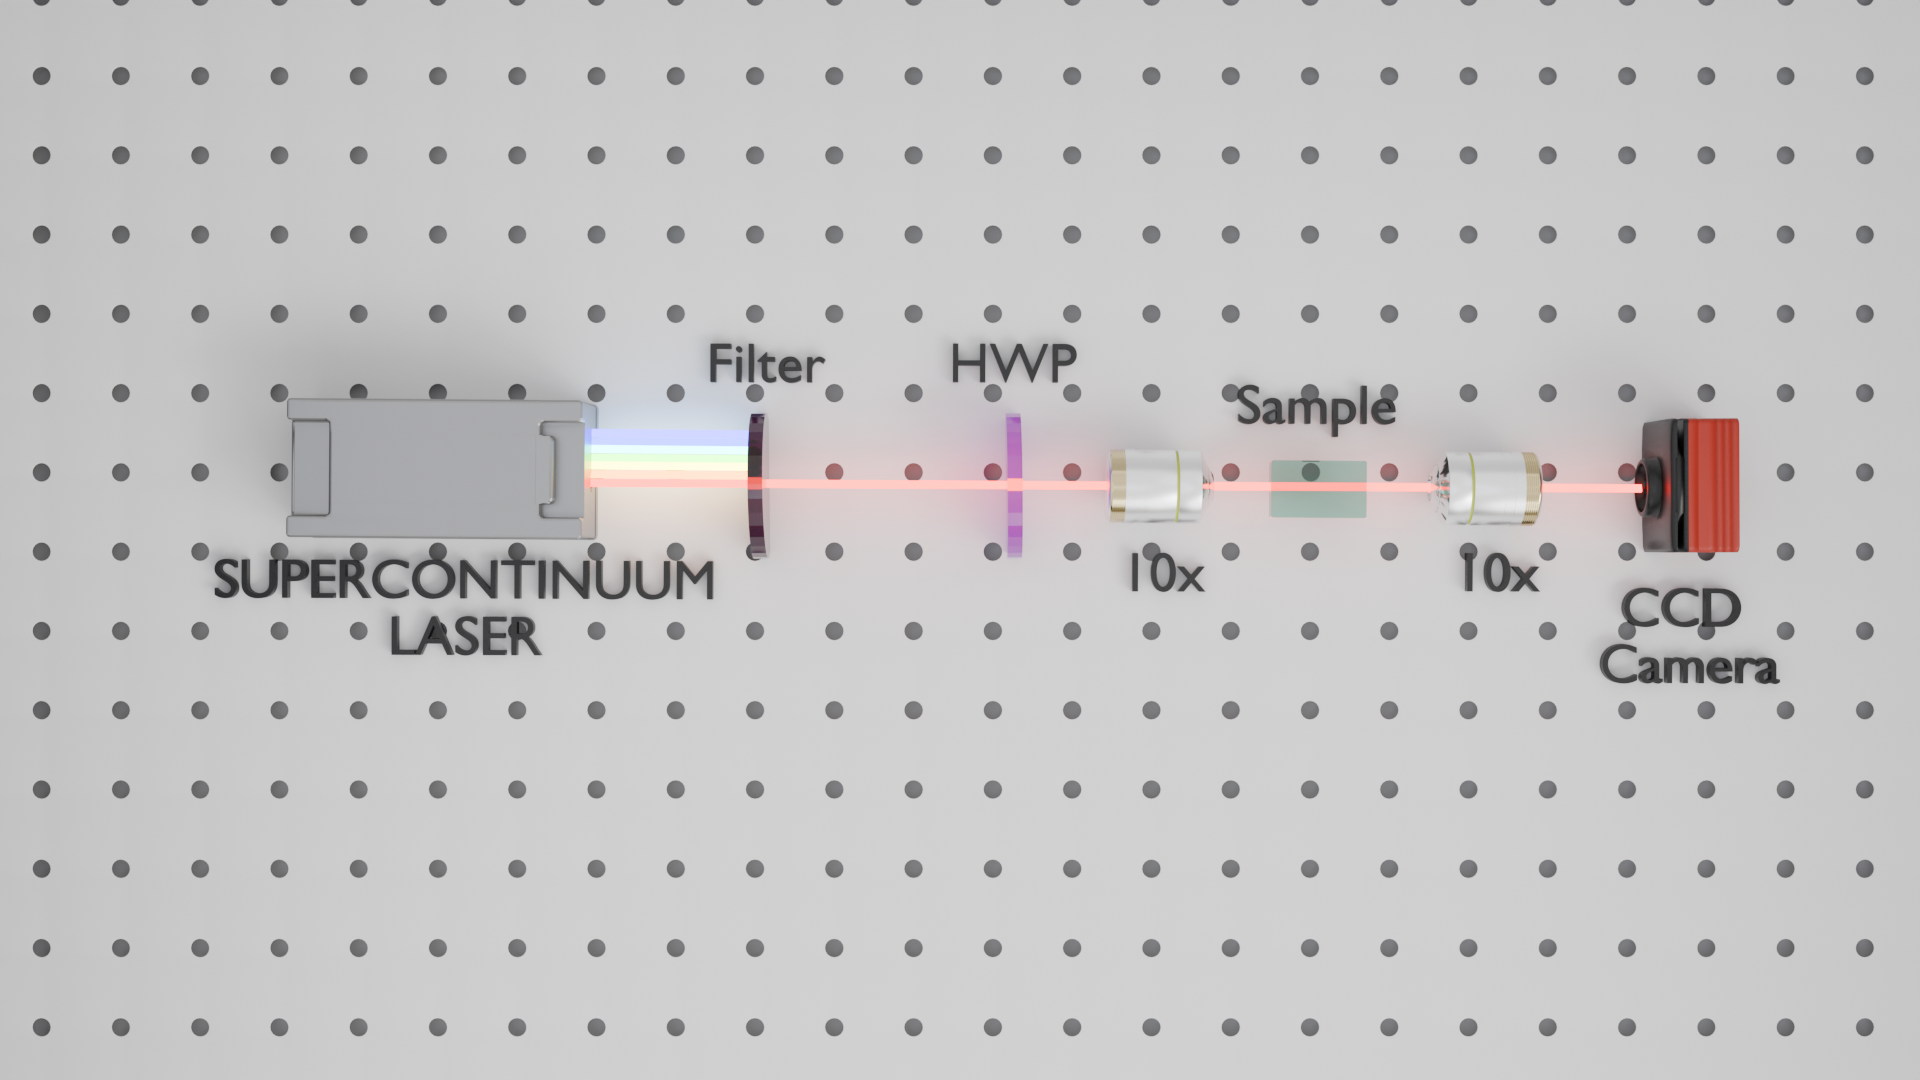
\includegraphics[width=\linewidth, trim={5cm 9cm 3cm 7cm},clip]{media/SC_setup}
    \caption[Supercontinuum laser excitation setup.]{Supercontinuum laser excitation setup. Filter: Acousto-optic modulator and iris. HWP: Half-wave plate.}
\end{figure}

To use initial conditions different from a Gaussian, it is necessary to incorporate methods of spatial light modulation. In this thesis, a technique known as phase encoding via hologram was implemented \citep{terhalle}.

\subsection{Premodulation Stage}
The spatial light modulator used is a HOLOEYE PLUTO-VIS SLM - Reflective LCOS (resolution 1920$\times$080 px, pixel size 8 $\mu$m), whose optical response occurs with polarization parallel to the optical table plane. A half-wave retarder ($\lambda/2$) followed by a Glan-Thompson polarizer 100,000:1 is used to ensure that the laser light polarization matches that of the SLM's response. Subsequently, the beam is magnified and collimated to cover the entire available pixel area using a 20x objective and a 100mm focal length lens (telescope).

\subsection{Modulation Stage}
A diffraction grating that maximizes the power of the first diffraction order is used. To modulate amplitude, the grating must be multiplied by the desired amplitude mask, while for phase modulation it suffices to add the grayscale level corresponding to the desired phase. Figure \ref{fig:SLMblaze} outlines the algorithm implemented in Python in Appendix \ref{sec:codeSLM}.

{
\sidecaptionvpos{figure}{c}
\begin{SCfigure}[]
    \centering
    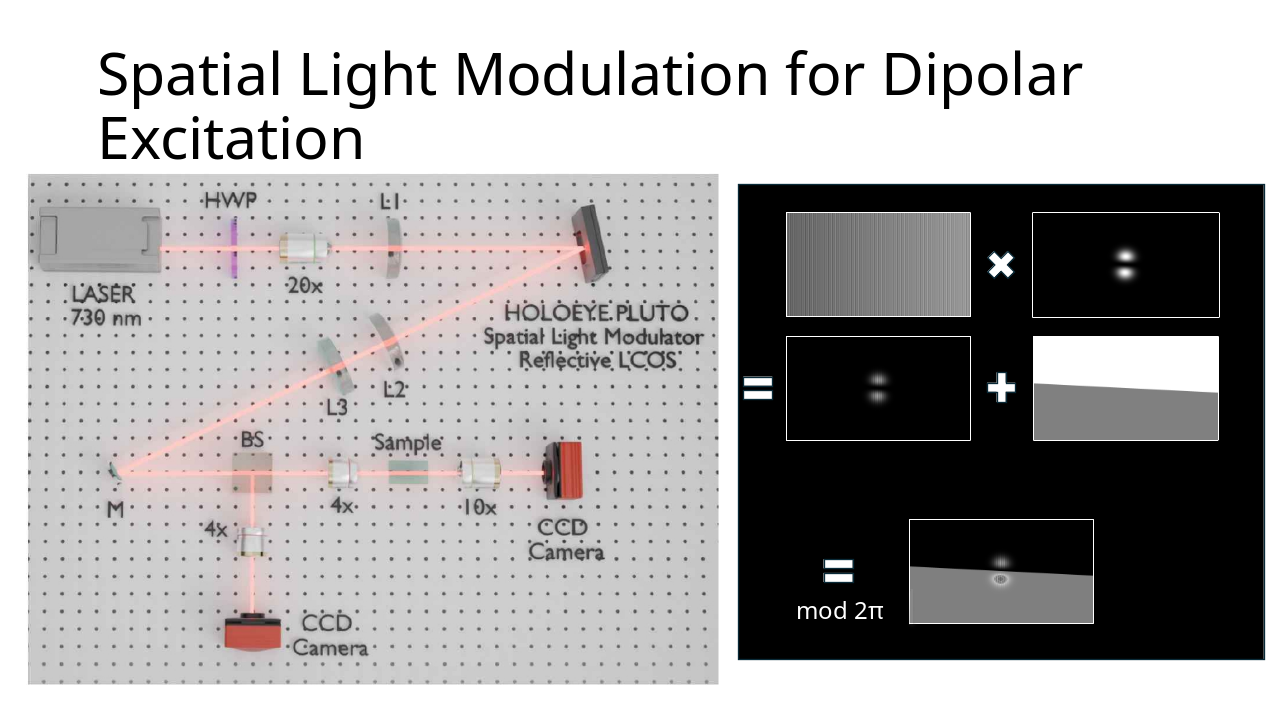
\includegraphics[width=0.35\linewidth, trim={19.5cm 0 0 5cm}, clip]{media/SLMblaze4.png}
    \caption[Spatial light modulation for arbitrary amplitude and phase masks.]{Spatial light modulation algorithm for arbitrary amplitude and phase masks. The diffraction grating parameters are subject to the wavelength used (730 nm).\label{fig:SLMblaze}}
\end{SCfigure}
}

\subsection{Coupling Stage}
The modulated image passes through a pair of lenses, $L_2$  with a 1000 mm focal length and $L_3$ with a 50 mm focal length, to reduce its size to the order of micrometers. The tilt of the sample's input face must coincide with the plane of the modulated image. To achieve this, two pairs of Gaussian beams are generated—one vertical and one horizontal—so that when translating the 4x objective lens, the interference maxima are produced at the midpoint between the centers of the Gaussian beams.

\subsection{Camera Capture Stage}
Once the sample tilt is calibrated, its position is fixed in the experimental setup. The output image is magnified using a 10x objective and captured using a beam profiler (Beam Profiler BC106N-VIS, Thorlabs) with a spatial resolution of 6.45 $\mu$m/px \citep{thorlabs_beam_profiler}.

\subsubsection{Optional Interferometric Configuration}
The setup can be modified to incorporate a Mach-Zehnder interferometer by:
\begin{itemize}
	\item A \textit{beam splitter} between lens $L_1$ and the SLM, using the pre-modulation beam as a reference.
	\item A second \textit{beam splitter} before the camera to recombine the beams.
	\item A neutral density (ND) filter to balance the intensities ($I_{\text{ref}} \approx I_{\text{muestra}}$).
\end{itemize}
For the generation of dipole modes, it is essential to adjust the phase difference between the recombined beams to a value close to ππ. This is experimentally evidenced by the appearance of an intensity minimum at the center of the interference pattern, corresponding to destructive interference in that region.

\subsection{Optical Circuit}
\begin{figure}[H]
	\centering
	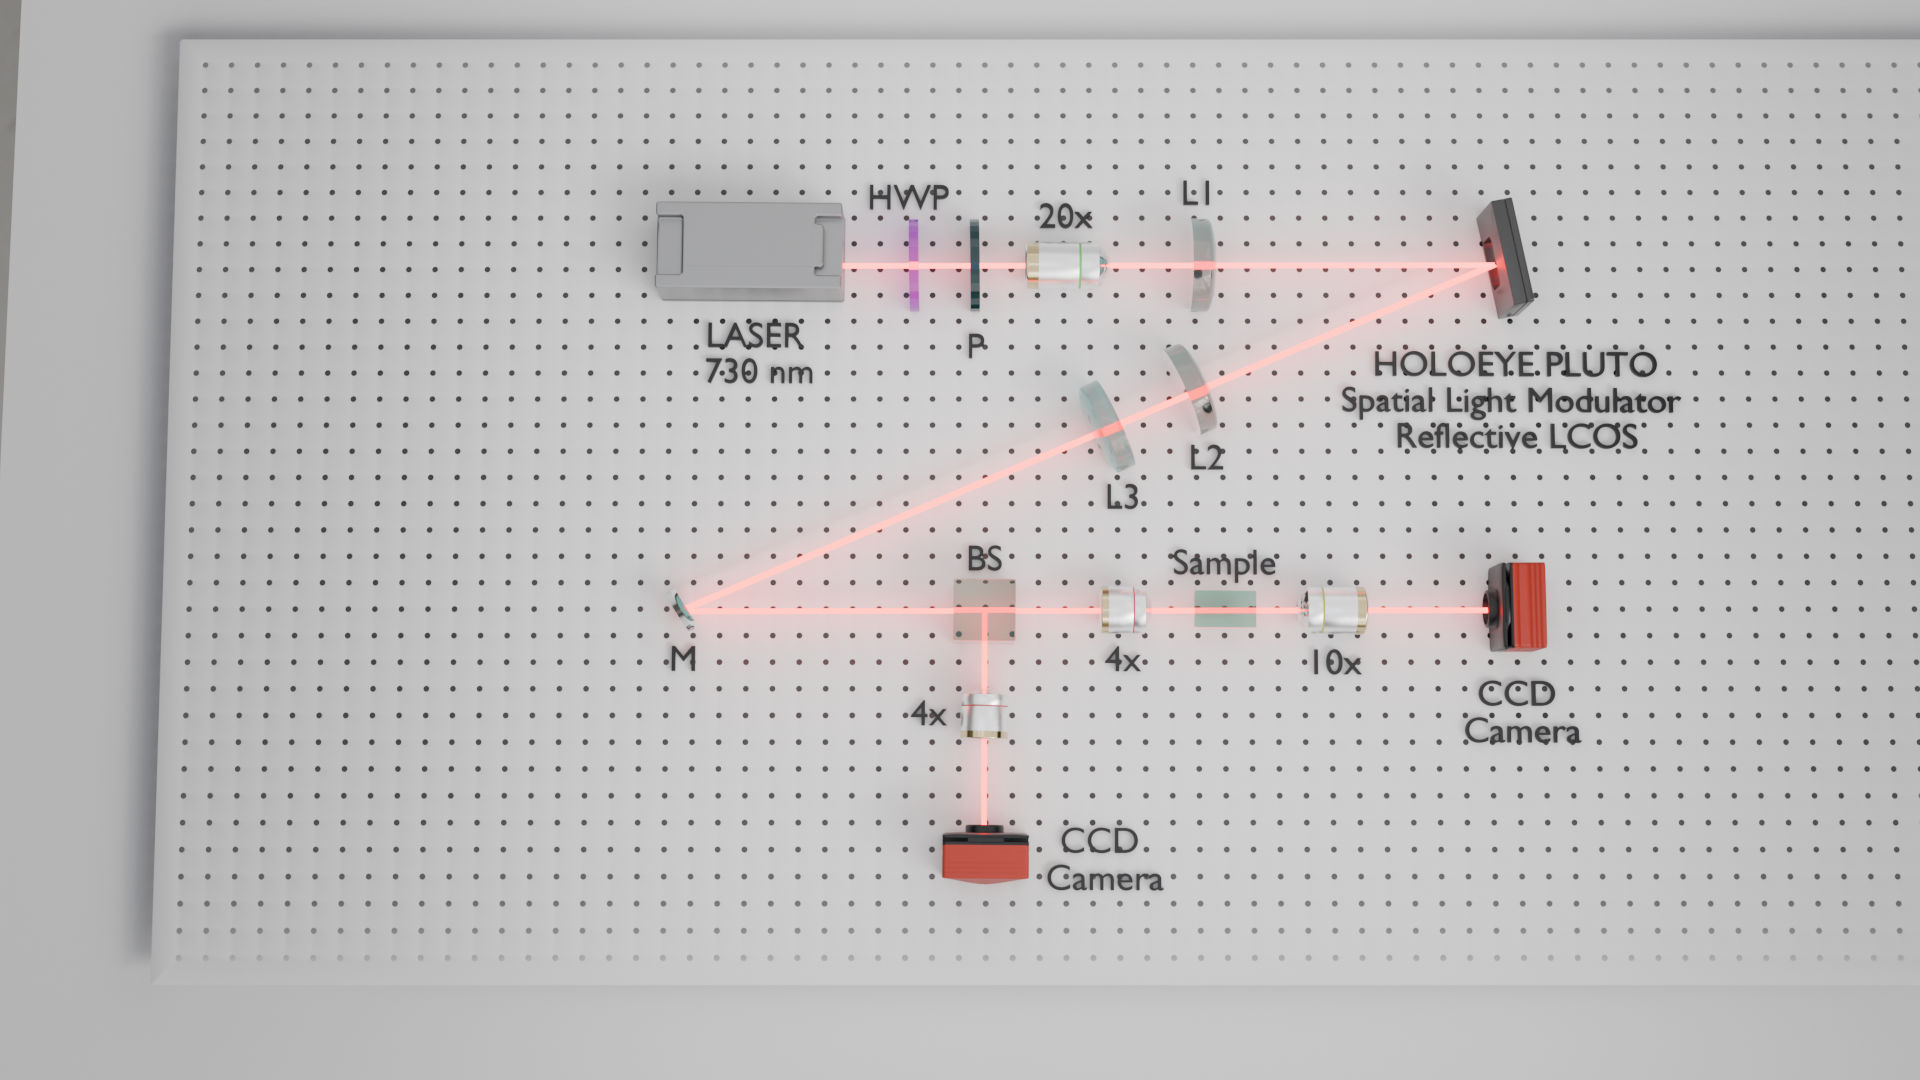
\includegraphics[width=0.8\linewidth, trim={21cm 5cm 7cm 5cm}, clip]{media/SLM_setupv1}
	\caption[Diagram of the spatial light modulation system]{Complete diagram of the experimental system for spatial light modulation, showing the optical components and their relative arrangements.}
	\label{fig:SLM_setup}
\end{figure}

\subsection{Generation of Complex Images \label{cap:oam}}
The capability for precise control over amplitude and phase is verified through the generation of optical vortices, quantified by their Orbital Angular Momentum (OAM). Interferometric analysis allows:
\begin{itemize}
	\item Determining the topological charge ℓℓ by counting the spiral branches in the interference pattern.
	\item Establishing the sign of ℓℓ through the direction of rotation of the phase front.
\end{itemize}

\begin{figure}[H]
	\centering
	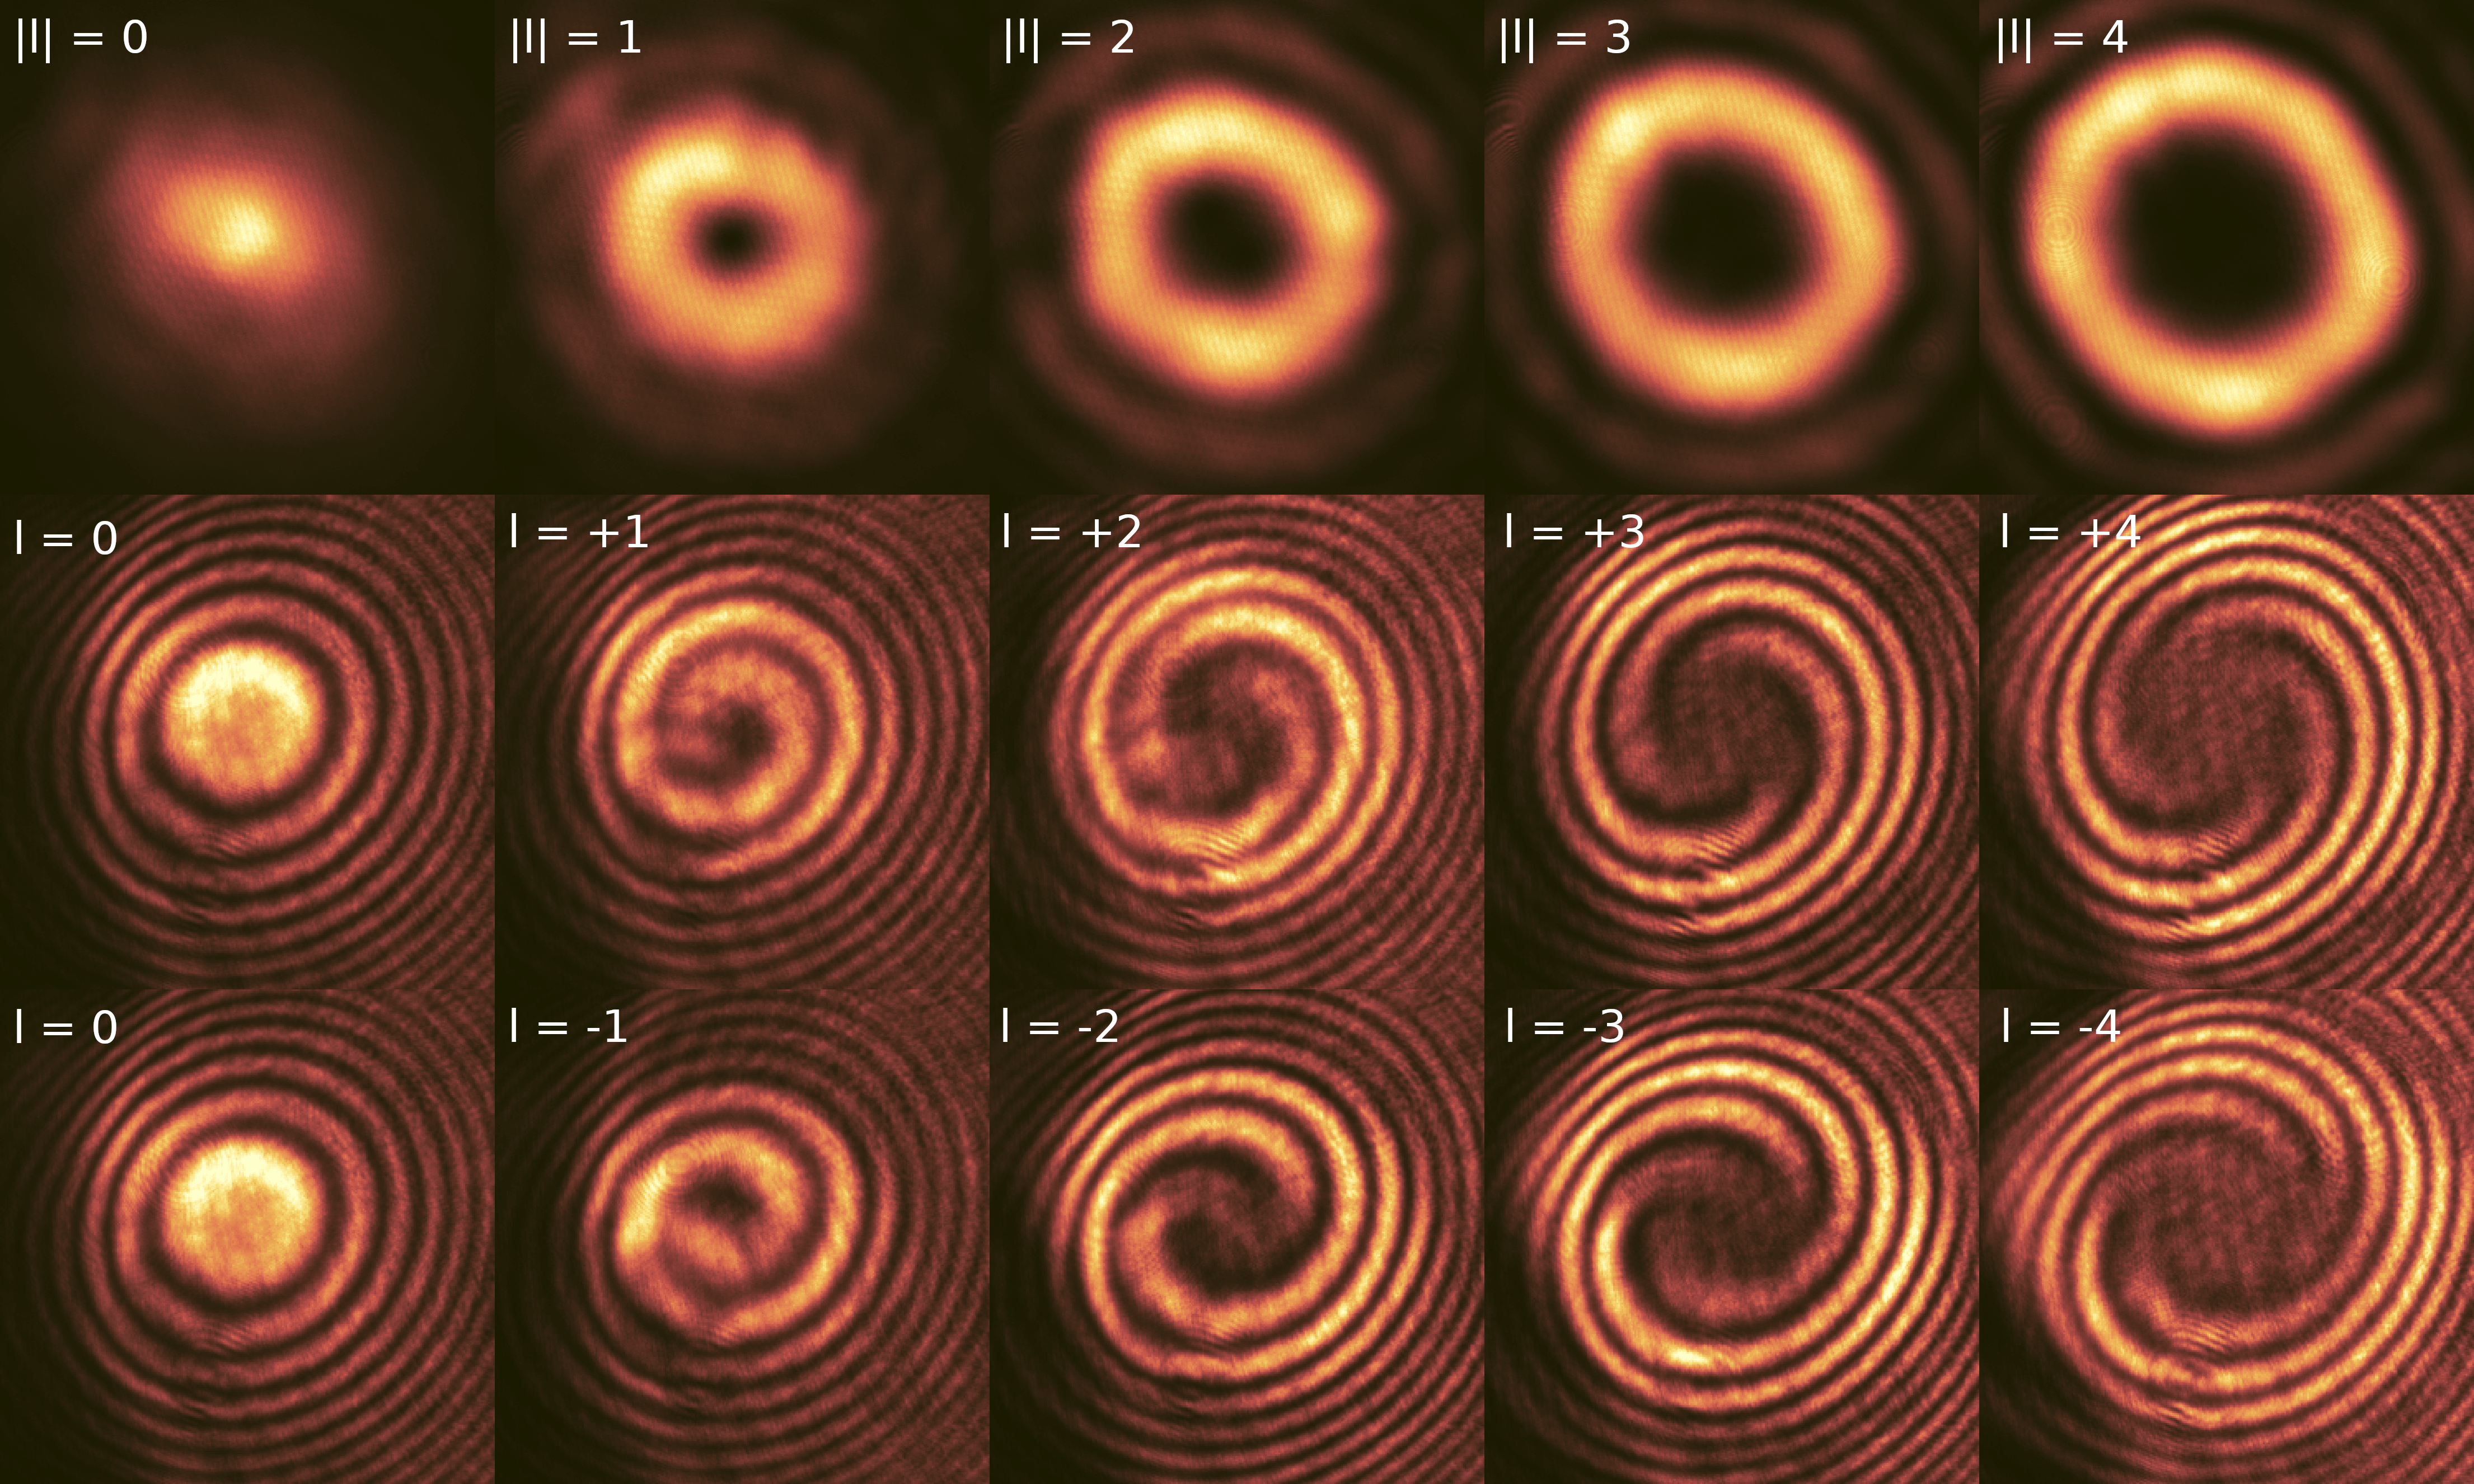
\includegraphics[width=0.8\linewidth]{media/OAM-free.png}
	\caption[Characterization of optical vortices via Mach-Zehnder interferometry.]{Characterization of optical vortices via Mach-Zehnder interferometry. \textbf{Top:} Intensity for different OAM charges ($\ell$). \textbf{Middle and Bottom:} Corresponding interference patterns, where the number of spiral branches indicates $|\ell|$ and the direction of rotation accounts for the sign of $\ell$.}
	\label{fig:OAM}
\end{figure}
\section{Image Analysis \label{sec:imageanal}}
From the captured images, it is possible to extract information about the power contained at each site of the discrete photonic system under study. To achieve this, the entire image must be divided into equally spaced rectangles that enclose the regions where waveguides are present, whether illuminated or not. The power at each site will then be the sum of the intensity of every pixel within its respective rectangle.

Image processing includes:
\begin{itemize}
	\item Background correction
	\item Normalization by maximum intensity.
	\item Automatic segmentation via thresholding.
\end{itemize}

The obtained data allow for the reconstruction of the power distribution within the photonic lattice and the analysis of coupling phenomena between neighboring waveguides.
\chapter{Coupling of $p_y$ Modes and the Invisibility Angle \label{cap:invisibility}}
In electrostatics, dipolar interactions can be described using second-order Legendre polynomials, particularly with $P_2(\cos(\theta))=3\cos^2(\theta)-1$, where $\theta$ epresents the angle between two electric dipoles. The angular value $\theta_m
\approx 0.62$ radians is known as the \textit{magic angle}, as it cancels the dominant dipolar interaction term \citep{medmagic}.

This chapter focuses on the experimental study of vertical dipolar modes, also referred to as $p_y$modes, whose existence requires surpassing the cutoff condition: a sufficiently short wavelength, combined with an index contrast $\Delta n$and an appropriate transverse dimension. These modes exhibit a transverse distribution characterized by two symmetric lobes relative to the horizontal axis and a phase difference of $\pi$ between them.

\section{Couplers}

When studying the evanescent coupling between $p_y$ modes in elliptical waveguides, two limiting configurations are distinguished: when the waveguides are arranged horizontally (aligned along the $x$-axis), the coupling—denoted $\varkappa_\pi$​—is positive; conversely, for vertical couplers (aligned along $y$), the coupling $\varkappa_\sigma$ eis negative \citep{Pmodecoupling}. This sign change is interpreted as an interference effect between the lobes of the $p_y$mode, whose lobular profile with odd symmetry about the horizontal axis generates different coupling conditions depending on the relative orientation of the waveguides.

This behavior presents an analogy\footnote{This analogy is purely geometric and modal. It does not imply the existence of electron clouds, interatomic potentials, or bonding energy in the chemical sense. However, it is retained as a useful conceptual tool to describe the relative orientation of the modes and the effect of symmetry on the strength and sign of the coupling. Its utility lies in the clarity with which it communicates differences in the nature of coupling, especially in multi-orbital systems like those studied in this thesis.} with the $\sigma$ and 
$\pi$ chemical bonds formed in carbon chains: in quantum chemistry, $\sigma$ bonds correspond to frontal (axial) overlaps of orbitals, while $\pi$ bonds arise from lateral overlaps, typically between $p$ corbitals with nodes along the bonding axis. Analogously, we refer here to \textit{coupling} $\varkappa_\sigma$ as that which occurs through axial superposition between modes with suitable symmetry, generating a profile without a transverse node; whereas \textit{coupling} $\varkappa_{\pi}$ or $\varkappa_{\theta = 0}$ corresponds to a lateral superposition, in which the modal distribution exhibits a central node.

To verify this effect, 20 dimers were experimentally fabricated with a fixed separation of 25 $\mu$m and a propagation length of 15 mm, varying the angle between waveguides from 0.00 rad to 1.57 rad. The initial excitation was generated using a spatial light modulator (SLM), programmed to selectively couple the $p_y$ mode into one of the waveguides.

\begin{figure}[H]
	\centering
	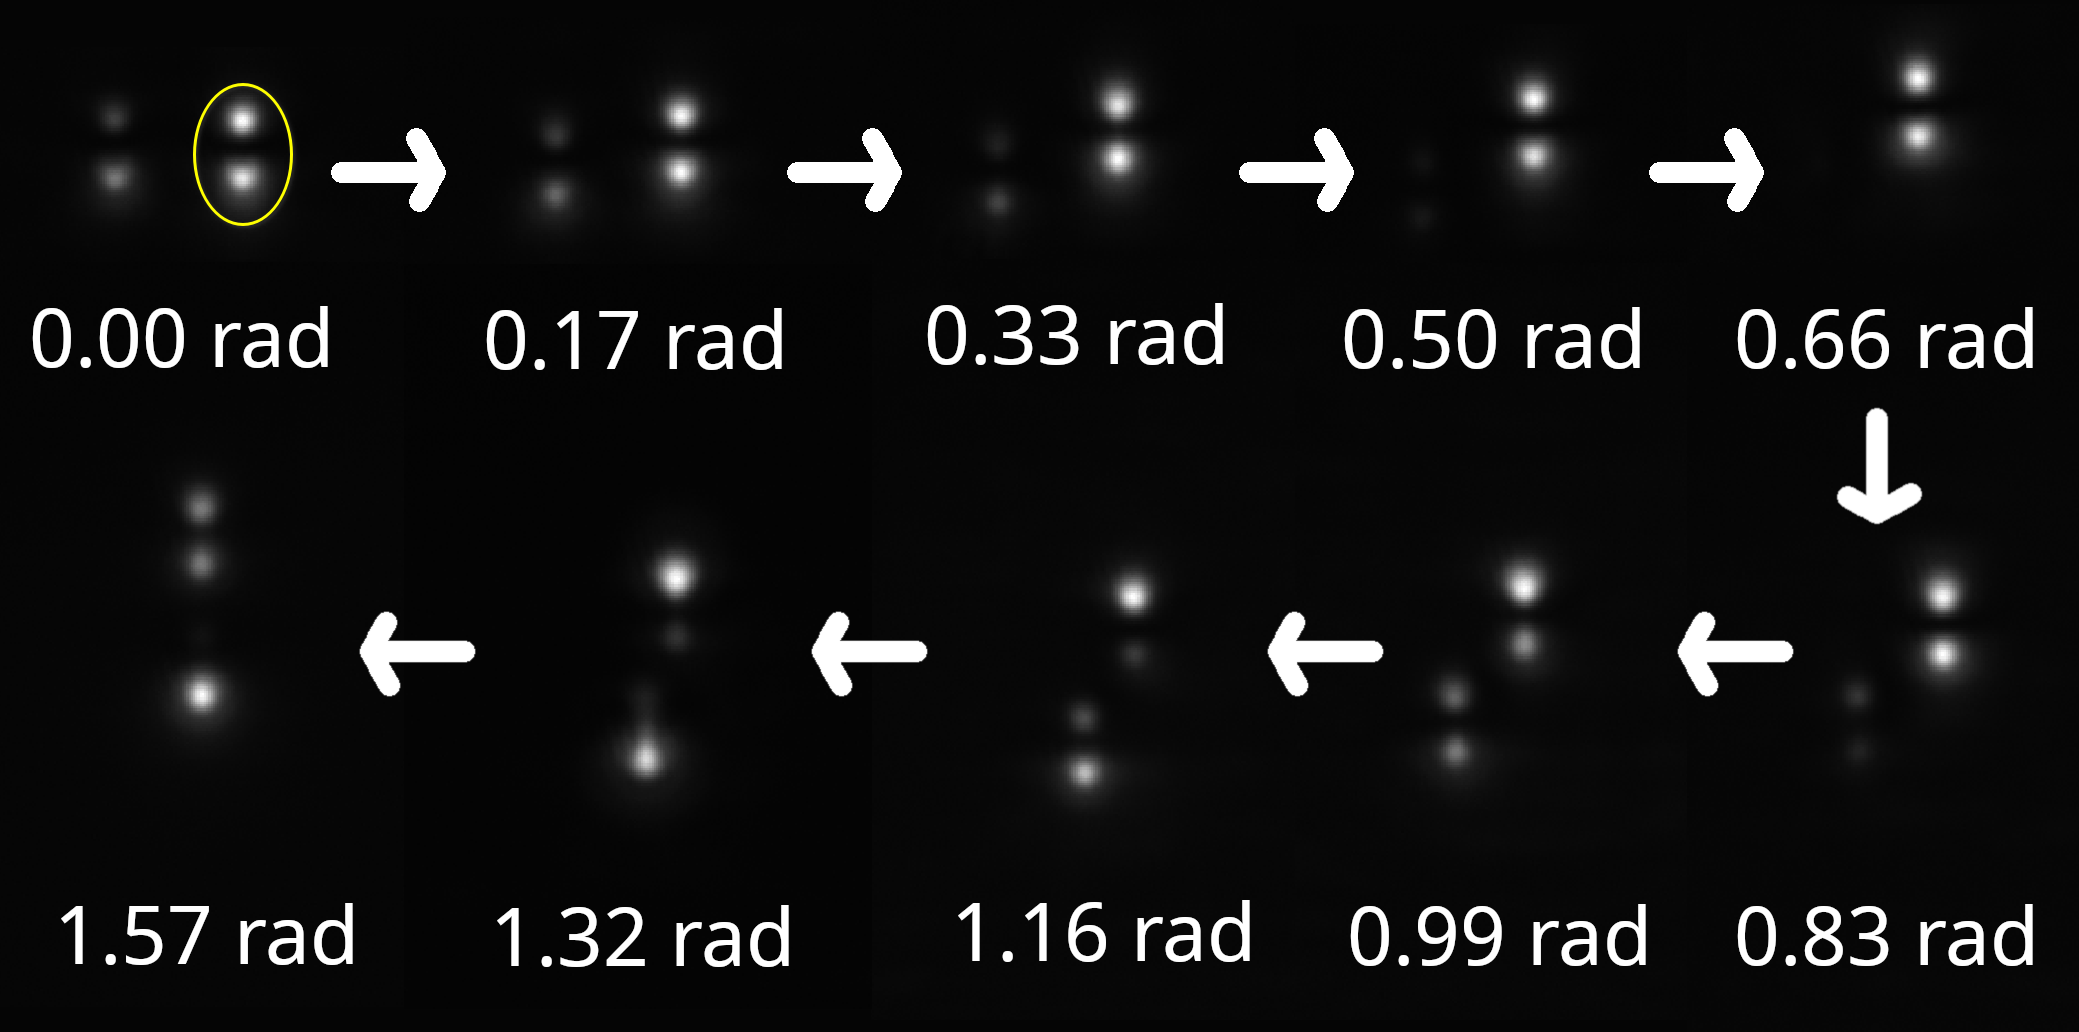
\includegraphics[width=0.7\linewidth]{media/26um_15mm_angles_v2.png}
\caption[Experimental angular sweep]{Experimental angular sweep for a propagation distance of 15 mm. The effect of the magic angle is observed between 0.50 and 0.66 rad. \label{fig:angulobarrido}}
\end{figure}

The obtained images were analyzed following the procedure described in Section~\ref{sec:imageanal}. Subsequently, using equation (\ref{eqn:coupling-simp}), which describes the dynamic coupling, the effective coupling was quantitatively characterized as a function of the angle $\theta$, measured from the horizontal. To correctly reflect the continuity of the coupling with the angle, the sign of the coupling was adjusted in the theoretical fit, as shown in Figure~\ref{fig:invisibility-coup}.
\begin{figure}[H]
    \centering
    
\includegraphics[width=0.6\linewidth]{codigo/eigenvalues_vs_angle.png}
   \caption[Propagation constants and angular couplings for P modes]{Propagation constants and couplings as a function of the angle for $p_y$modes, numerically calculated using EME. The results are compared with experimental data extracted from Figure \ref{fig:angulobarrido}. \label{fig:invisibility-coup}}
\end{figure} \vspace{-2ex}
\section{Honeycomb Lattices}
The honeycomb lattice, known for being the underlying crystalline structure of graphene, presents properties relevant to this thesis, particularly in its Bloch bands: both are dispersive and exhibit a Dirac point \citep{honeycombdirac}. Once the fabrication parameters from the previous section were determined, the same effect was studied in a honeycomb lattice by keeping the distance between sites constant while varying the angle (Figure \ref{fig:HCLBW}).

\begin{figure}[H]
	\centering
	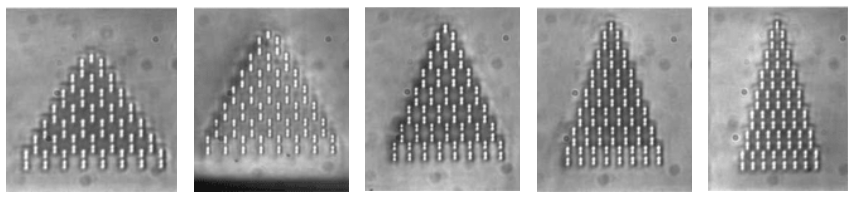
\includegraphics[width=\linewidth]{media/honeycomb_lattices_bw.png}
	\caption[Microscope images of honeycomb-type photonic lattices for P modes]{Microscope images of honeycomb-type photonic lattices for $p_y$ modes under white light illumination. \label{fig:HCLBW}}
\end{figure} \vspace{-3ex} A first-neighbors model would only consider the vertical coupling $\varkappa_\sigma$ and the angular coupling $\varkappa_\theta$. However, an accurate description of the experimental data requires including couplings up to third neighbors, as well as non-orthogonality corrections. Figure~\ref{fig:honeycombmodel} shows a schematic of the complete model. The system's Hamiltonian is expressed as:
\begin{equation}
	\hat{H}_\Sigma = \hat{H}_{NN} + \hat{H}_{NNN} + \hat{H}_{NNNN},
\end{equation}
where $\hat{H}_{NN}$, $\hat{H}_{NNN}$ and $\hat{H}_{NNNN}$ contain the couplings to first neighbors ($\varkappa_\sigma$ y $\varkappa_\theta$), second neighbors ($t_\pi$ and $t_{\theta 2}$), and third neighbors ($t_{\theta 1}$ y $t_{\theta 3}$), respectively (see Figure \ref{fig:honeycombmodel}).

\begin{figure}[H]
	\centering
	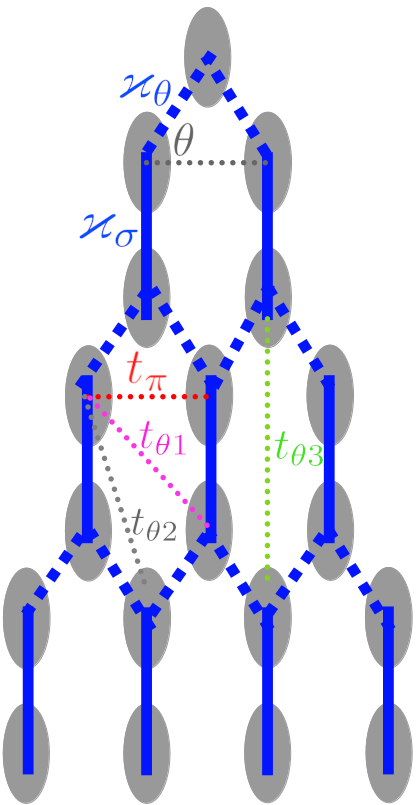
\includegraphics[width=0.25\linewidth]{media/honeycomb-lattice.png}
	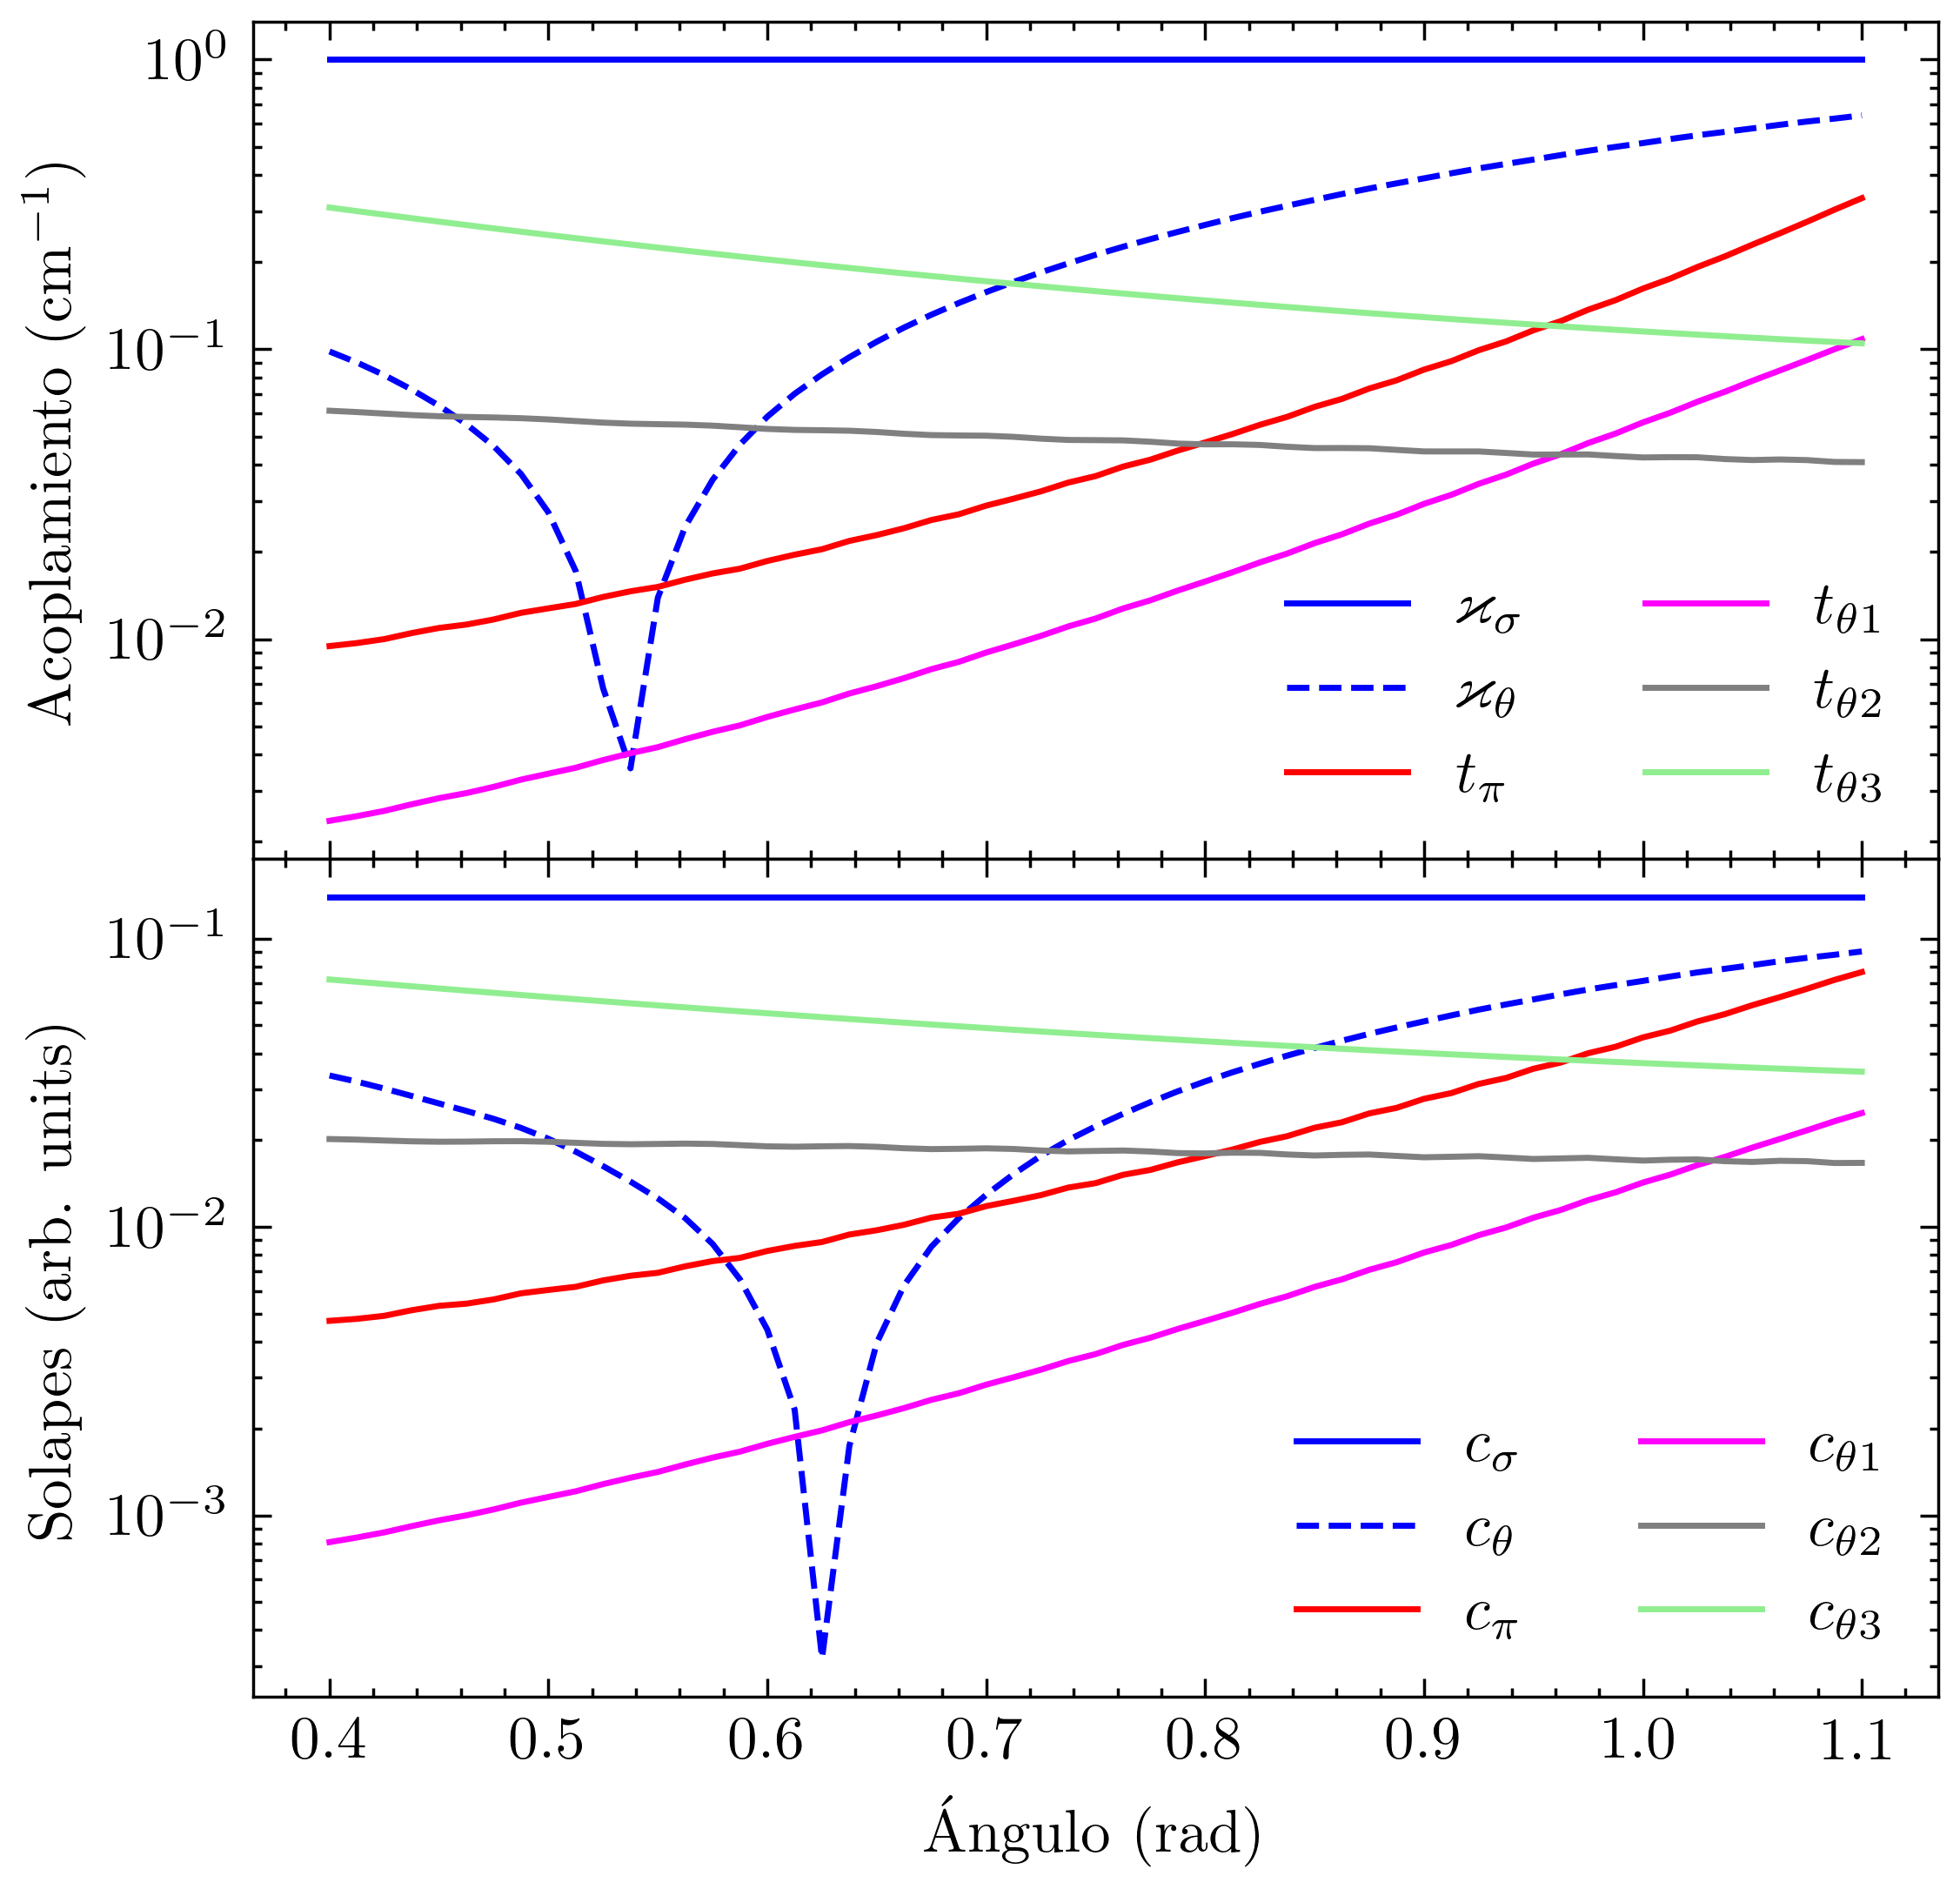
\includegraphics[width=0.55\linewidth]{codigo/NNNN_overlap_vs_angle.png}
	\caption[Honeycomb model for $p_y$ modes with couplings up to third neighbors]{\textbf{Left:} Schematic of the honeycomb model for $p_y$ modes with couplings up to third neighbors. \textbf{Right:} (Top) Absolute values of the couplings as a function of the angle $\theta$. (Bottom) Normalized overlap integrals as a function of the angle $\theta$.\label{fig:honeycombmodel}}
\end{figure} \vspace{-3ex} Furthermore, the non-orthogonal matrix $\hat{c}$ is defined from the matrix $\hat{P}$ [equation~(\ref{eqn:CMTnum})] as $c_{ij} = P_{ij}/I$, where $I = P_{ii}$ is the intensity of the $p_y$ mode, so that the diagonal elements of $\hat{c}$ are equal to 1. Similarly to the couplings, Figure \ref{fig:honeycombmodel} plots the magnitude of the overlaps $c_{ij}$ eas a function of the angle.
The non-Hermitian Hamiltonian $\hat{H}_\Sigma' \equiv \hat{c}^{-1} \hat{H}_\Sigma$ describes the dynamics of the lattice and incorporates both non-orthogonal effects and long-range couplings. Figure \ref{fig:honeycomb-spectra} shows the spectrum as a function of the angle $\theta$. Two main regions are distinguished: one for angles $0.4 < \theta < 0.7$, where the eigenvalues cluster into three quasi-flat bands, and another for angles $0.7 < \theta < 1.1$, where the gap decreases in magnitude, thus increasing transport in the lattice. The inverse participation ratio (IPR) of each eigenstate is calculated as $\text{IPR} = \sum_i I_i^2/(\sum_i I_i)^2$. This allows for an adequate description of the experimental data shown in the right panel of Figure \ref{fig:honeycomb-spectra}.
\begin{figure}[H]
	\centering
	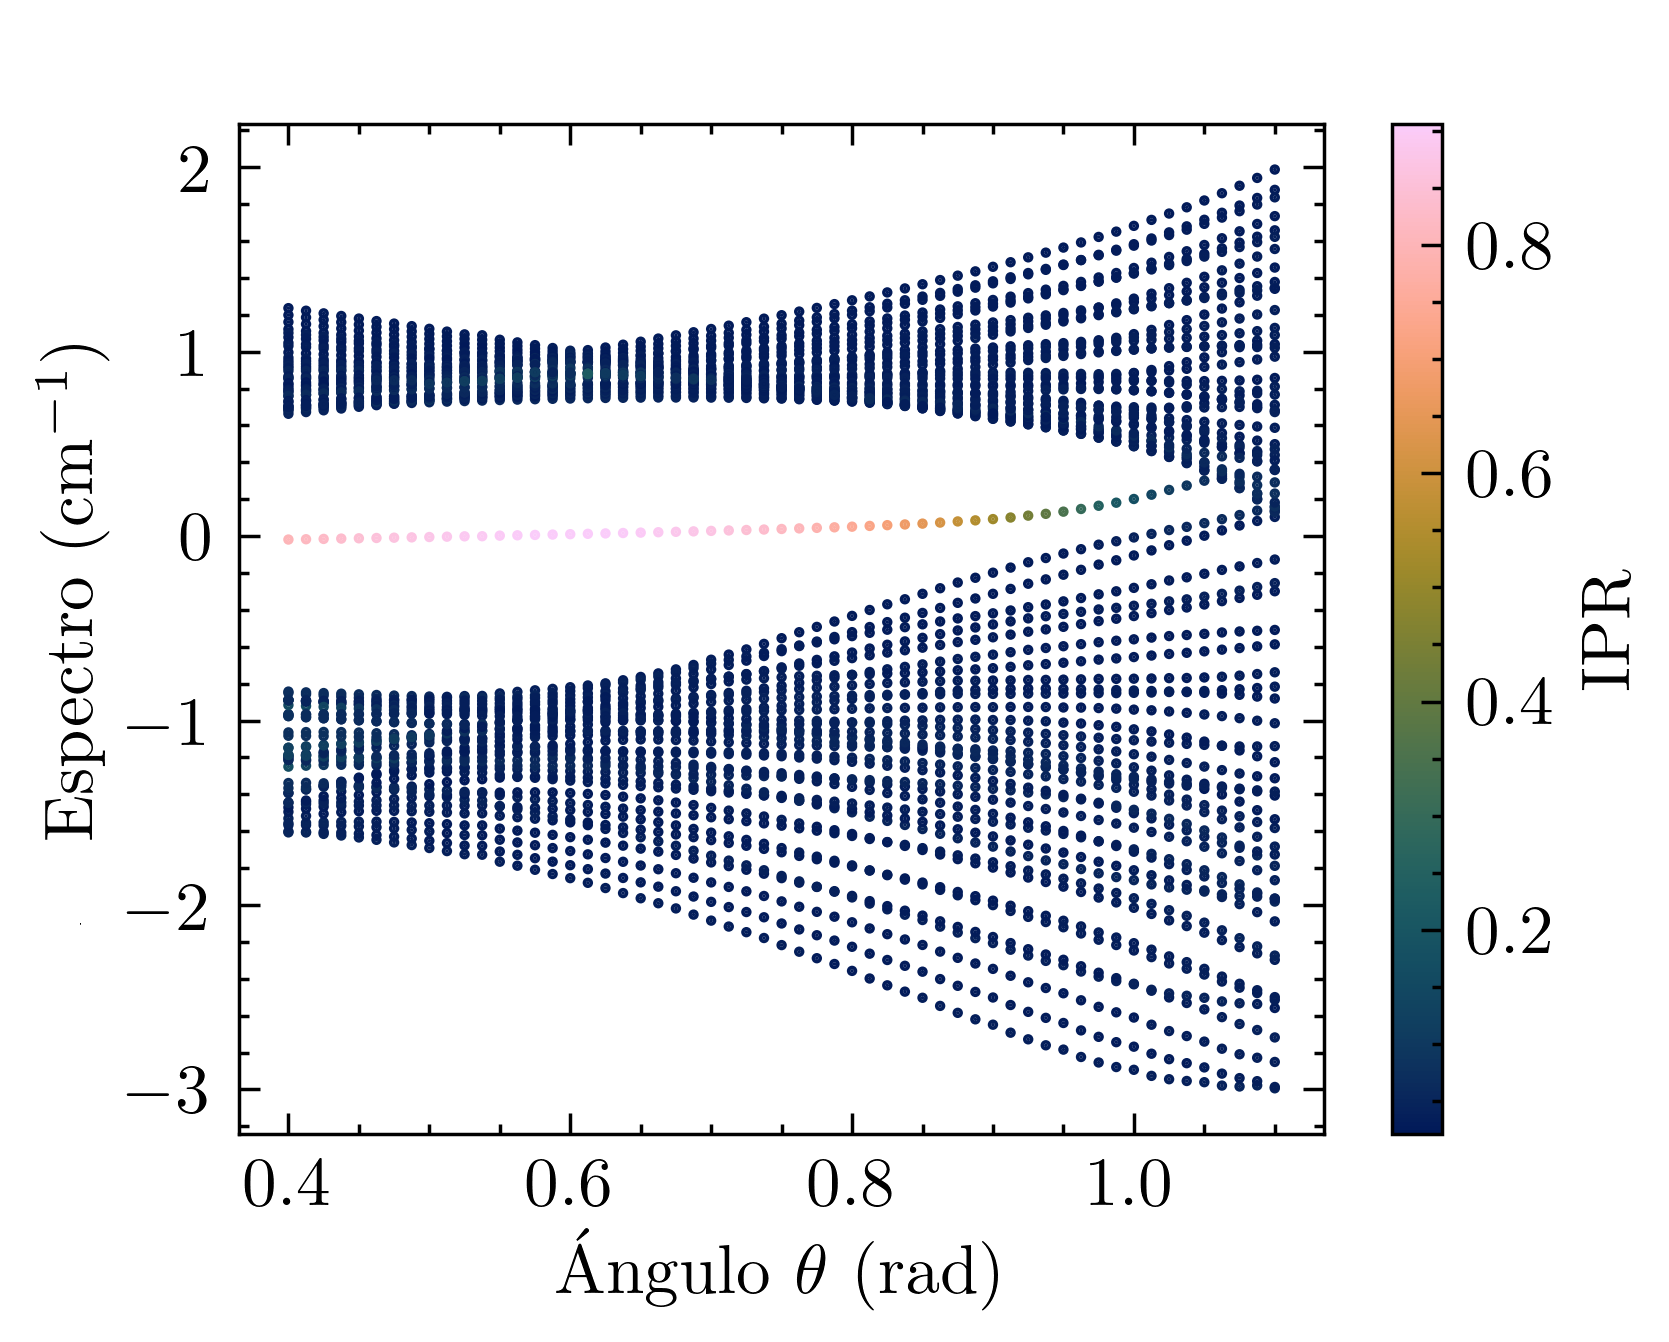
\includegraphics[width=0.45\linewidth]{codigo/honeycomb_eigenvalues_vs_angle.png}
	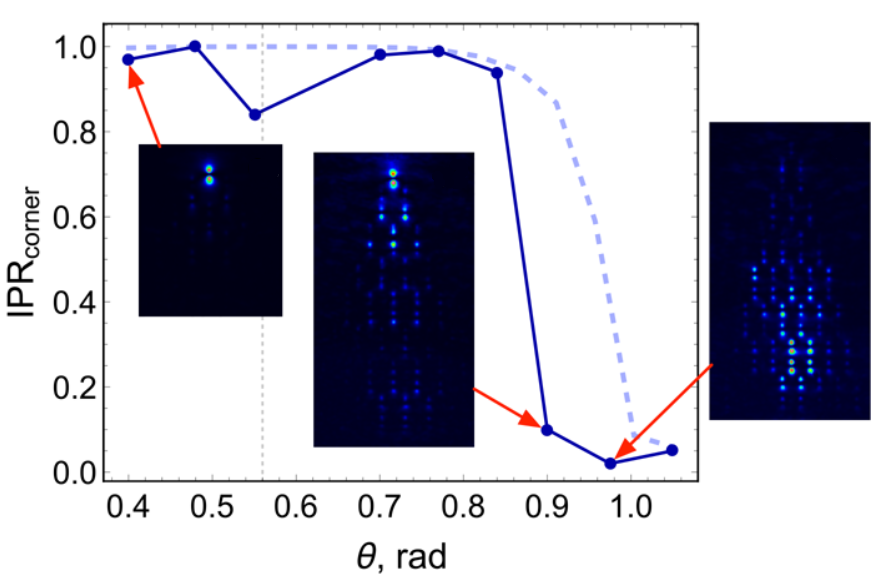
\includegraphics[width=0.5\linewidth]{media/ipr-corner-exp.png}
	\caption[Spectrum of the honeycomb lattice of $p_y$ modes as a function of the angle]{\textbf{Left:} Spectrum of the matrix $\hat{H}_\Sigma'$ as a function of the angle. Each point is colored according to its inverse participation ratio (IPR). \textbf{Right:} Inverse participation ratio for the corner site excitation as a function of the angle $\theta$.\label{fig:honeycomb-spectra}}
\end{figure} \vspace{-3ex}
The strong localization observed when exciting the corner site is explained by the fact that the projection of the initial condition onto the eigenstates corresponds predominantly to the eigenstate with a null eigenvalue. The existence of this eigenstate is due to the topology exhibited by the Hamiltonian $\hat{H}_\Sigma'$ in reciprocal or Bloch space. Although it is possible to calculate the bulk polarization using Wilson loops and determine that its value is discretized as $\mathbf{P} = (0.5, 0.5)$, it is more illustrative to note that the lattice can be decomposed into quasi-SSH chains (see Figure \ref{fig:quasi-ssh}). In both schemes, quantization is a consequence of the inversion symmetry present in the lattice.
\begin{figure}[H]
	\centering
	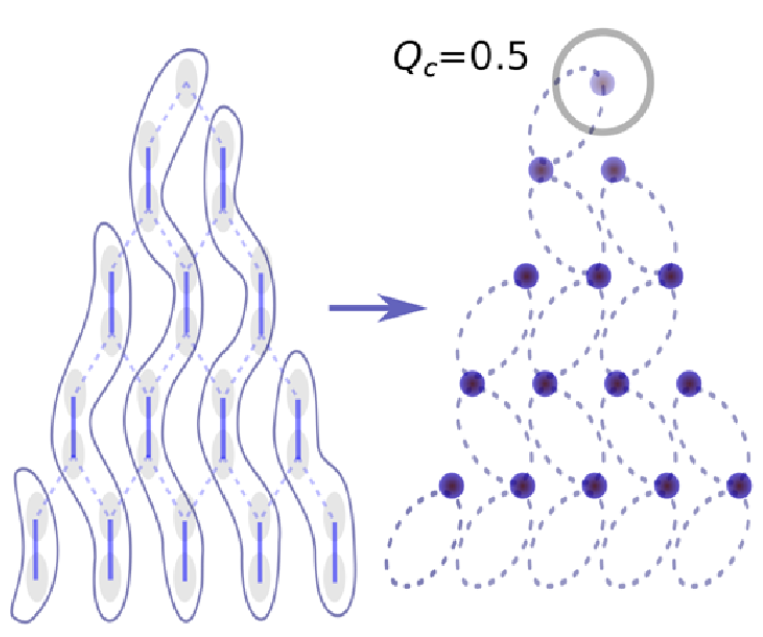
\includegraphics[width=0.40\linewidth]{media/cuasi-ssh.png}
	\hfill
	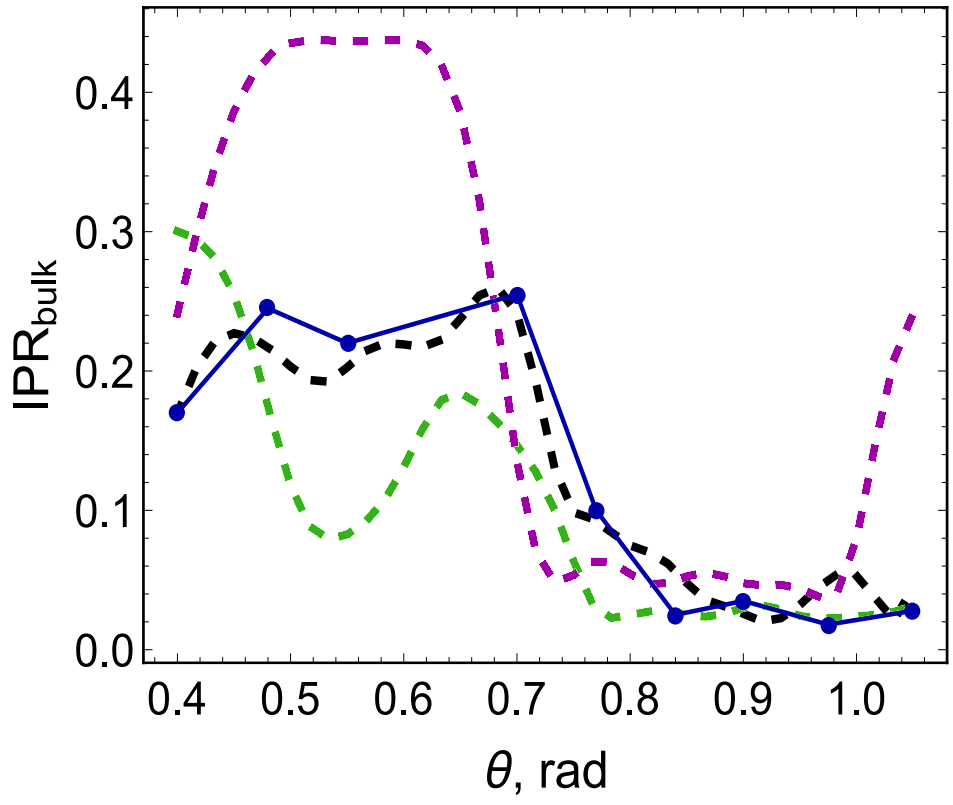
\includegraphics[width=0.40\linewidth]{media/ipr-bulk-exp.png}
	\caption[Decomposition of the lattice into quasi-SSH chains]{
		\textbf{Left: }
		Decomposition of the lattice in the flat-band limit into isolated dimer SSH chains. \textbf{Right: } IPR for the experimental excitation of the central site of the lattice (points connected with lines to guide the eye) and numerically simulated for three cases: without long-range couplings and non-orthogonal corrections (dashed purple curve), with long-range couplings but without non-orthogonal corrections (dashed green curve), and with long-range couplings and non-orthogonal corrections (dashed black curve). \label{fig:quasi-ssh}}
\end{figure} \vspace{-2ex}
The dynamics associated with flat bands were studied experimentally through the localized excitation of a single site within the bulk of the lattice, with the aim of extracting the value of the \textit{Inverse Participation Ratio} (IPR). Because a point-like excitation has components in all Bloch bands, this type of initial preparation amplifies the differences in the dispersion of each band. In this context, propagation with very little diffraction indicates that all involved bands are nearly flat. This approach allows for the direct observation of the bulk properties of the lattice, as a central excitation avoids edge effects and favors the manifestation of the global modal structure. In the ideal limit, a system composed solely of perfectly flat bands would not allow transverse transport, restricting dynamic evolution to local oscillations between effective dimers.

The analyzed data reveal two distinct regimes: for lattices with $0.4 < \theta < 0.8$ (close to the invisibility angle), a good confinement effect (\emph{caging}) is observed. However, larger angles ($\theta > 0.8$) favor significant field diffraction, resulting in delocalization at the output. These experimental results (points in Figure \ref{fig:quasi-ssh}) agree with theoretical calculations (dashed line). Contrary to expectations, long-range couplings and non-orthogonality corrections do not degrade the flat band dynamics near the invisibility angle; rather, they complement each other. The maximum IPR values ($0.20$-$0.25$) for the dimer state after three Aharonov-Bohm caging cycles \cite{abcagingseba} indicate localization comparable to one-dimensional optical proposals with all their bands flat (ABF).

In conclusion, this experimental study demonstrates that the \textit{invisibility angle}—defined as the angular condition for the suppression of dipolar coupling between $P$ modes—constitutes an effective tool for controlling transport in discrete photonic lattices. By exploiting the transverse symmetry of the modes as an active resource, optical confinement is achieved without the need for disorder, nonlinearity, or external fields. These results strengthen the conceptual framework of multi-orbital lattices as versatile platforms for studying flat band dynamics and controlled confinement through geometry and modal symmetry.

\chapter{Non-Symmetric Evanescent Coupling}
\label{cap:asymmetric}

Discrete models in photonics, such as coupled-mode theory (CMT), often assume symmetric couplings between waveguides, meaning that the coupling constant between two sites \( C_{i \to j} \) is equal to \( C_{j \to i} \). This assumption ensures the Hermiticity of the effective Hamiltonian and is typically justified when the waveguides are identical and sufficiently separated. However, this symmetry can be inherently broken in real systems, even in the absence of loss or gain, when the waveguides exhibit different refractive index profiles, which is experimentally achieved by varying the writing power of the waveguides \cite{nonsymm}.

\section{Origin of Non-Symmetric Dynamics}

Evanescent coupling between waveguides occurs due to the overlap of the modal tails outside the confinement core. When two waveguides have different index contrasts (\( \Delta n_1 \ne \Delta n_2 \)), the guided modes exhibit evanescent tails with varying amplitude and extent, which induces a directionally unequal coupling: \( C_{1 \to 2} \ne C_{2 \to 1} \).
\begin{figure}[H]
	\centering
	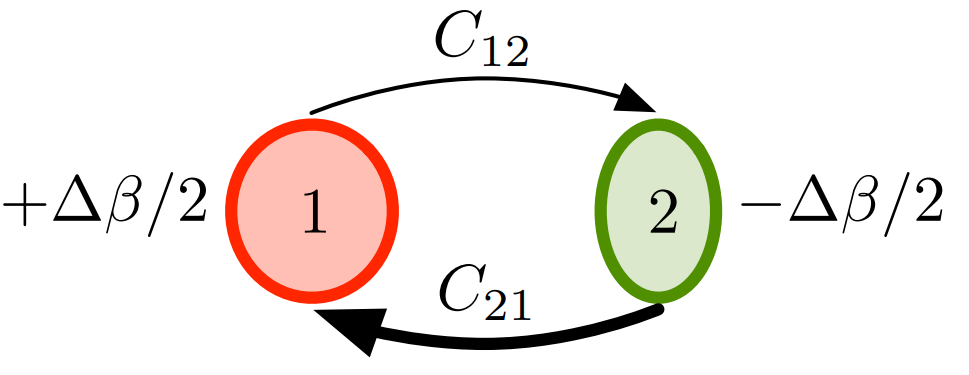
\includegraphics[width=0.4\linewidth]{media/nonsympaper}
	\caption{Schematic of non-symmetric coupling.}
\end{figure}
This \textit{non-symmetric} behavior can be quantified using the generalized non-orthogonal coupled-mode theory developed in Section~\ref{cap:CMTteo}, which includes the effect of modal overlap through the matrix \( \hat{P} \), encoding power normalization.

Considering a dimer composed of two non-identical waveguides, the dynamic equations for the modal amplitudes are written (see equation~(\ref{eqn:non-ortho-CMT-eqs})) as:
\begin{equation}
	-i
	\frac{d}{dz}
	\begin{pmatrix}
		P_{11} & P_{12} \\
		P_{12} & P_{22}
	\end{pmatrix}
	\begin{pmatrix}
		u_1 \\
		u_2
	\end{pmatrix}
	=
	\begin{pmatrix}
		H_{11} & H_{12} \\
		H_{12} & H_{22}
	\end{pmatrix}
	\begin{pmatrix}
		u_1 \\
		u_2
	\end{pmatrix}
	\iff
	-i\frac{d}{dz}\textbf{v} = \hat{H}' \textbf{v} \ ,
\end{equation}
where \( \textbf{v} = \hat{P}^{1/2} \textbf{u} \) represents an orthogonalized basis, and \( \hat{H}' = \hat{P}^{-1/2} \hat{H} \hat{P}^{-1/2} \) is the effective Hamiltonian in that basis. Since \( \hat{H} \) and \( \hat{P} \) are symmetric, \( \hat{H}' \) is also symmetric, which guarantees real eigenvalues. By proposing stationary solutions of the form \( \textbf{v}(z) \sim e^{i\lambda z} \), the generalized eigenvalue problem $\det(\hat{H} - \lambda \hat{P}) = 0$  is obtained.
It is important to emphasize that this orthogonalized basis \( \textbf{v} \) is not experimentally accessible: in a real setup, only modes localized in individual waveguides can be observed, which corresponds to the physical basis \( \textbf{u} \). Therefore, the experimental analysis of the dynamics must be performed in this basis, where the evolution is governed by the effective coupling matrix:
\begin{equation*}
	\hat{C} = \hat{P}^{-1} \hat{H} = \frac{1}{P_{11}P_{22} - P_{12}^2}
	\begin{pmatrix}
		P_{22}H_{11} - P_{12}H_{12} & P_{22}H_{12} - P_{12}H_{22} \\
		P_{11}H_{12} - P_{12}H_{11} & P_{11}H_{22} - P_{12}H_{12}
	\end{pmatrix}.
\end{equation*}
This system exhibits non-reciprocal dynamics: the energy transfer efficiency depends on the input channel. This asymmetry can be quantified experimentally through the \textit{intensity imbalance}, defined for each excitation \( i = L, R \) as:
\begin{equation*}
	I^i(z) \equiv \frac{P^i_1(z) - P^i_2(z)}{P^i_1(z) + P^i_2(z)} \ ,
\end{equation*}
and its absolute average as:
\begin{equation*}
	\bar{I}(z) \equiv \frac{|I^L(z) + I^R(z)|}{2} \ .
\end{equation*}
The quantity \( \bar{I}(z) \) is particularly useful for detecting global asymmetries in the dynamics: any deviation from zero implies a non-symmetric evolution, revealing the presence of non-reciprocal evanescent couplings.

\section{Numerical Validation}

Using the Eigenmode Expansion (EME) method (Section~\ref{cap:eme}), the dynamics of asymmetric dimers were simulated by injecting the same Gaussian initial condition in all cases. Figure~\ref{fig:nonotrho-num} shows the absolute average of intensity imbalances $\bar{I}(z)$ as a function of distance for $n_2 - n_1 = 1.75 \times 10^{-5}$ (weak asymmetry) and for $n_2 - n_1 = 5.00 \times 10^{-5}$ (strong asymmetry).

\begin{figure}[H]
	\centering
	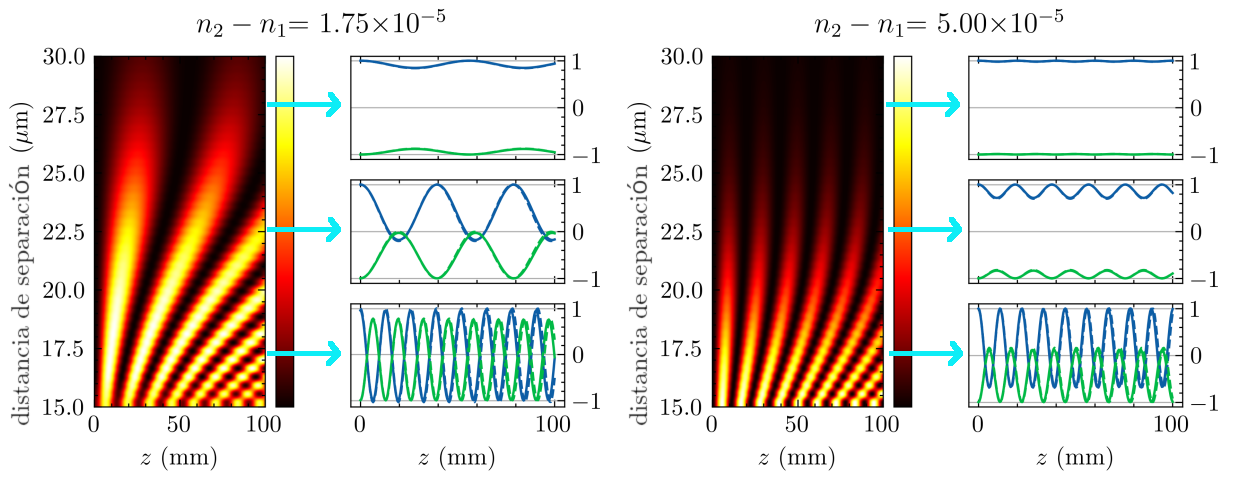
\includegraphics[width=\linewidth]{media/imbalance-nonortho.png}
	\caption[Absolute average of intensity imbalances $\bar{I}(z)$ as a function of propagation distance zz]{Absolute average of intensity imbalances $\bar{I}(z)$ as a function of propagation distance zz and the separation distance between waveguides, comparing two regimes: (1) weak asymmetry  ($\Delta n = 1.75 \times 10^{-5}$) and (2) strong asymmetry ($\Delta n = 5.00 \times 10^{-5}$). The values $I^L$ (green) and $I^R$ (blue) corresponding to three specific study cases are included.}
	\label{fig:nonotrho-num}
\end{figure}
\section{Experimental Verification}
To verify this effect, dimers were fabricated using the femtosecond laser writing technique described in Section \ref{cap:fs}, varying the input channel \( i \), the writing power \( P_{g}^i \), the distance between waveguides \( d \), and the effective propagation length \( z \). In particular, the case \( \Delta P = P_g^1 - P_g^2 = 5\,\mathrm{mW} \) was explored, with a separation  \( d = 18\,\mu\mathrm{m} \). Figure~\ref{fig:nosymexp} shows that excitation of the upper waveguide favors energy transfer to the lower waveguide, while the inverse excitation achieves a 1:1 energy distribution at $z\sim 11$ mm.
\begin{figure}[H]
	\centering
	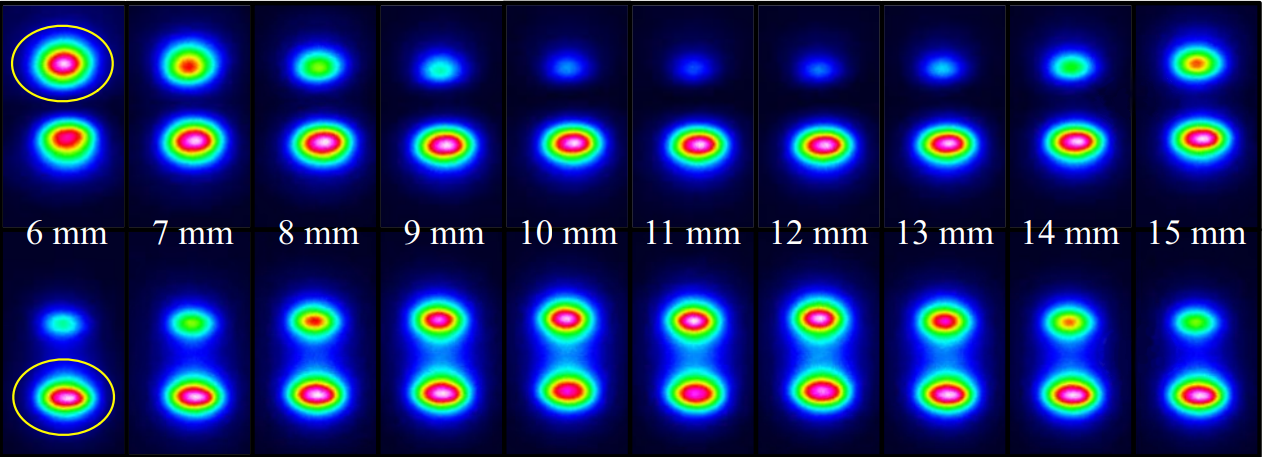
\includegraphics[width=0.9\linewidth]{media/nonsymm-exp.png}
	\caption[Output profiles for different propagation lengths.]{Output profiles for different propagation lengths  \( z_i \), exciting the upper waveguide (left) and lower waveguide (right), with \( d = 18\,\mu\mathrm{m} \). \label{fig:nosymexp}}
\end{figure} \vspace{-4ex} Using slab-type waveguides and TE modes (see Section \ref{cap:slab}), analytical expressions for the couplings are obtained:
\begin{equation*}
	\frac{C_{21}}{C_{12}} \approx \left( \frac{\Delta n_2}{\Delta n_1} \right)^2 e^{(\gamma_2 - \gamma_1) d}\approx \frac{P_2^1(z)}{P_1^2(z)} \ ,
\end{equation*}
where \( \gamma_i \) represents the evanescent decay coefficient of mode \( i \). his expression shows that the asymmetry increases with the separation between waveguides, with the difference between the modal decay rates $\gamma_2 - \gamma_1$ and with the square of the ratio of index contrasts $\Delta n_2/\Delta n_1$. 

\section{Implications and Applications}

This study demonstrates that non-symmetric coupling is a physical phenomenon that, in the absence of energy loss or gain, can be passively induced. Its implications include: \textit{breakdown of reciprocity}, without requiring magneto-optical materials or temporal modulation; \textit{modal asymmetry}, since the inequality between \( C_{ij} \) and \( C_{ji} \) affects the formation of symmetric/antisymmetric states and interference; \textit{directional optical devices}, such as asymmetric beam splitters or optical isolators; and its \textit{extension to lattices} with directed couplings. Together, these results allow for an extension of coupled-mode theory and open new opportunities in the design of optical lattices with directional functionality.
\chapter{Photonic Molecules \label{cap:molecules}}
The technique of writing waveguides using ultrashort laser pulses, described in Chapter~\ref{cap:fs}, allows for the three-dimensional fabrication of photonic structures with micrometric precision. However, this technique has inherent limitations due to the elliptical shape of the laser focus, which imposes restrictions on the transverse modes that can be efficiently excited and, in particular, on the possible intermodal couplings between modes of different symmetry, such as $S$ and $P$ \citep{interorbital}.

To overcome these restrictions and expand the degrees of freedom in the design of photonic networks, an approach inspired by molecular physics is adopted here: by positioning two waveguides sufficiently close, their modes can couple coherently, generating new extended collective modes. This process is analogous to molecular formation in quantum physics, where two atomic orbitals combine linearly to form bonding and antibonding molecular orbitals (see Figure \ref{fig:molec-anal}).

In this work, we will call a \textit{photonic molecule} a system of two coupled waveguides, whose eigenfunctions combine to generate symmetric and antisymmetric hybrid modes, in analogy with molecular orbitals. This analogy is based on the spatial shape of the modes and their controlled overlap, but does not imply the existence of bonding forces, shared electrons, or interatomic potentials. The relationship with quantum molecules is, therefore, formal and geometric, and is restricted to the structural parallelism between optical modes and orbitals \citep{molecules}.

\begin{figure}[H]
	\centering
	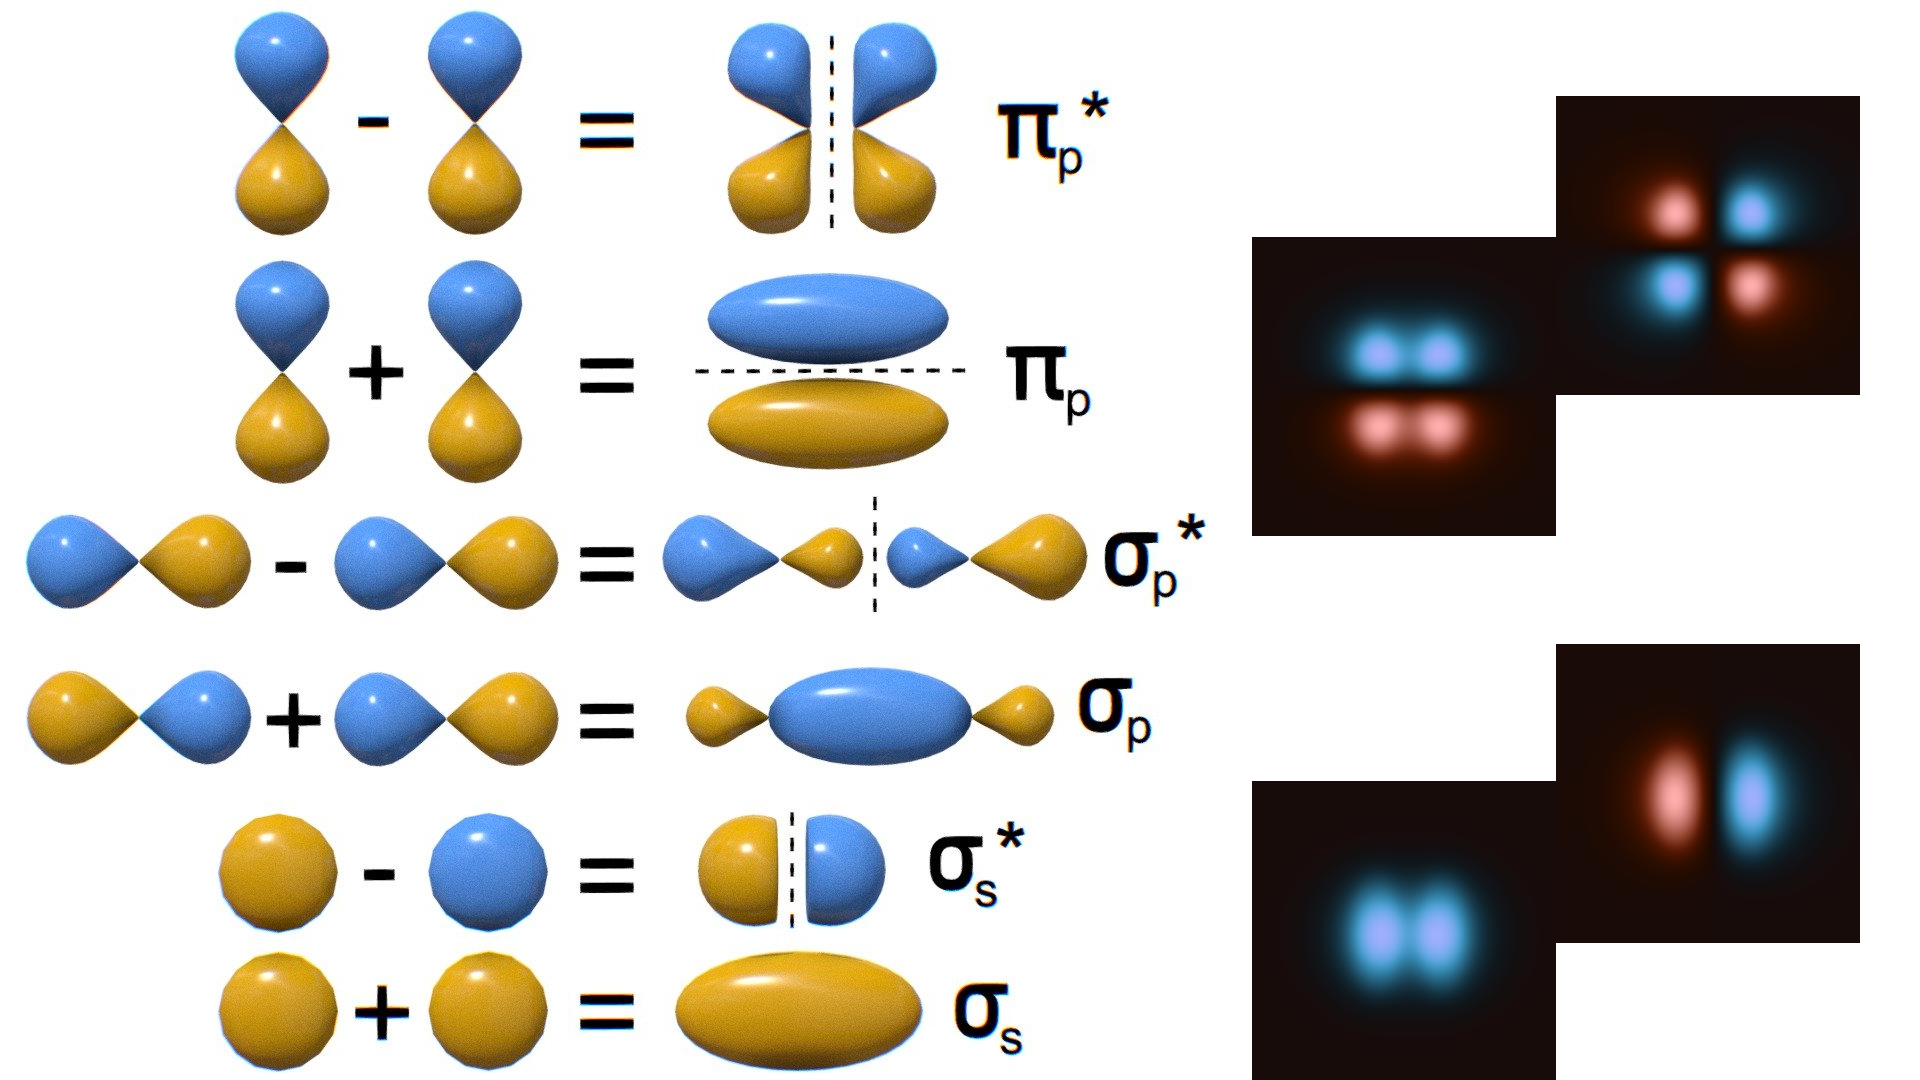
\includegraphics[width=0.6\linewidth]{media/moleculas.png}
	\caption[Analogy and differences between quantum molecules (left) and photonic molecules (right).]{Analogy and differences between quantum molecules (left) and photonic molecules (right). Both atomic orbitals and individual waveguide modes can hybridize, generating new collective states. In the photonic case, hybridization occurs between guided optical modes. Here, there is no photonic analogue of the $\sigma_p$ molecular orbitals. \label{fig:molec-anal}}
\end{figure}

Building on this idea, this chapter experimentally analyzes a photonic lattice constructed from such molecules as basic building blocks. In particular, a periodic SSH-type lattice \citep{SPSSH} is studied—a multi-orbital extension of the Su-Schrieffer-Heeger model—which allows exploring the impact of interorbital $S\hspace*{-0.3ex}P$ coupling on band topology. The system exhibits two independent topological transitions, associated with the modulation of geometric dimerization and the detuning between modes of different symmetry. These transitions are characterized through the observation of edge modes, the calculation of bulk polarization, and spectral analysis, enabling access to a rich photonic phenomenology based on modal engineering.

\section{Eigenstates of the Photonic Coupler for Small Separation Distances}

As mentioned in Section~\ref{cap:CMT}, coupled-mode theory (CMT) adequately describes the photonic systems under study when the distance between waveguides exceeds $13\,\mu$m. or smaller separations, the system must be treated as a single macro-waveguide. The eigenmode expansion (EME), presented in Section~\ref{cap:eme}, provides a numerical tool valid for both regimes. Through simulations of waveguide pairs at different distances, the behavior of their eigenstates was characterized. Figure~\ref{fig:molecule-coup} shows that the antisymmetric eigenstate ($+-$) only exists for distances greater than $13\,\mu$m, as below this threshold it becomes a radiation mode ($k_z^{+-} < k_0 n_0$). In contrast, the symmetric eigenstate ($++$) ersists and can be described as a single entity, which in this thesis will be referred to as the \textit{S mode} of the photonic molecule.
\begin{figure}[H]
	\centering
	
\includegraphics[width=0.9\linewidth]{media/eigenvalues_vs_angle.png}
	\caption[Propagation and couplings in photonic molecules]{
		\textbf{Left:} Propagation constants and couplings as a function of distance for fundamental modes, calculated using EME.
		\textbf{Right:} Propagation constants of $S$ and $P$ modes as a function of wavelength.
		\label{fig:molecule-coup}}
\end{figure}
Although the propagation constants of the $S$ and $P$ modes in the same molecule exhibit different values, they can be equalized between adjacent molecules by adjusting the refractive index contrast in the waveguides \citep{interorbital, SPSSH}. For example, Figure~\ref{fig:molecule-coup} shows that at $730$\,nm the propagation constants are equalized for $\Delta n_S = 5.200 \times 10^{-4}$ and $\Delta n_P = 10.423 \times 10^{-4}$.

\section{Photonic Molecules in the SP-SSH Lattice}

For the experimental implementation (Section~\ref{cap:fs}) of a lattice exhibiting SP coupling \citep{interorbital, toporusos, SPSSH}, the horizontal $P$ modes from the previous section, obtained through photonic molecules, were used. Precise tuning of the propagation constants of the $S$ ($k_z^S$) and $P$ ($k_z^P$) modes allowed considering a degree of freedom analogous to electron spin (\textit{pseudospin}). The Hamiltonian $H$ of this lattice \citep{SPSSH}, illustrated in Figure~\ref{fig:sp-ssh-model}, is as follows:
\begin{align*}
	H &= \sum_n \left[\frac{\delta\beta}{2} \left( p^*_{n, 1} p_{n, 1} - s^*_{n, 1} s_{n, 1} + p^*_{n, 2} p_{n, 2} - s^*_{n, 2} s_{n, 2} \right) + \varkappa_{ss, 2}s^*_{n, 2} s_{n, 1} - \varkappa_{pp, 2}p^*_{n, 2} p_{n, 1} \right. \\
	&+ \varkappa_{ss, 1} \left( s_{n-1, 2}^*s_{n, 1} + s_{n+1, 2}^*s_{n, 2} \right) - \varkappa_{pp, 1} \left( p_{n-1, 2}^*p_{n, 1} + p_{n+1, 2}^*p_{n, 2} \right) + \varkappa_{sp, 2} \left( s_{n, 2}^* p_{n, 1} - p_{n, 2}^* s_{n, 1} \right) \\
	&+ \left. \varkappa_{sp, 1} \left( s_{n-1, 2}^* p_{n, 1} - p_{n-1, 2}^* s_{n, 1} + s_{n+1, 1}^*p_{n, 2} - p_{n+1, 1}^* s_{n, 2} \right) \right] + \text{c.c.}
\end{align*}

\begin{figure}[H]
	\centering
	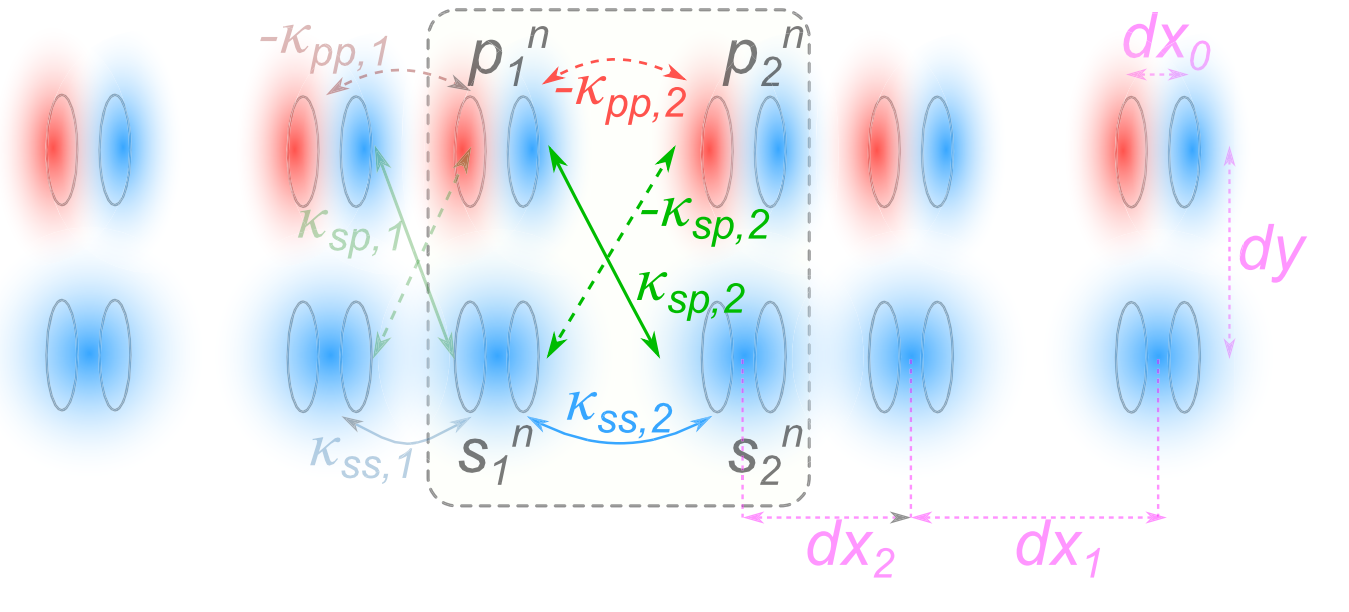
\includegraphics[width=0.7\linewidth]{media/ssh_sp_model}
	\caption{Schematic of the SP-SSH lattice and the considered couplings. \label{fig:sp-ssh-model}}
\end{figure} \vspace{-2ex}
If the basis $\mathbf{v}^n = \left( s_1^n, p_1^n, s_2^n, p_2^n \right)^T$is chosen, the Bloch Hamiltonian can be written in block form as:
\begin{equation*}
	\hat{H}(k) = \begin{pmatrix}
		\hat{\beta} & e^{-ika} \hat{\varkappa}_{1-} + \hat{\varkappa}_{2+} \\
		e^{ika} \hat{\varkappa}_{1+} + \hat{\varkappa}_{2-} & \hat{\beta}
	\end{pmatrix} \ ,
\end{equation*}
donde $\hat{\beta} = \frac{k_z^S - k_z^P}{2} \hat{\sigma}_z$ y $\hat{\varkappa}_{i\pm} = \begin{pmatrix}
	\varkappa_{ss, i} & \pm\varkappa_{sp, i} \\
	\mp\varkappa_{sp, i} & - \varkappa_{pp, i}
\end{pmatrix} \ .$

\section{Topology in the SP-SSH Lattice}
The SP-SSH model allows exploring new topological phases beyond the conventional SSH model, as it incorporates two orbitals ($S$ and $P$ modes) whose linear combinations can be interpreted as a pseudospin. It becomes necessary to study the topology of the system since the spectrum of the Hamiltonian is insufficient to fully explain the behavior of this system, particularly due to the appearance of zero-energy edge states. By applying the unitary transformation
\begin{equation*}
	\hat{U} = \frac{1}{\sqrt{2}}\begin{pmatrix}
		1 & 1 & 0 & 0 \\
		0 & 0 & 1 & -1 \\
		1 & -1 & 0 & 0 \\
		0 & 0 & 1 & 1
	\end{pmatrix} \ ,
\end{equation*} 
it becomes clearer how to interpret the system. In particular, for $\Delta\beta = 0$ and $\varkappa_{ss,1}=\varkappa_{pp,1}$ we have:
\begin{equation*}
	\hat{H} = \begin{pmatrix}
		\hat{H}_+ & 0 \\
		0 & \hat{H}_-
	\end{pmatrix} \ ,
\end{equation*} 
with
\begin{equation*}
	\hat{H}_\pm = \begin{pmatrix}
		0 & e^{-ika}(\varkappa_{ss,1}\mp \varkappa_{sp,1}) + (\varkappa_{ss,2}\pm \varkappa_{sp,2}) \\
		e^{ika}(\varkappa_{ss,1}\mp \varkappa_{sp,1}) + (\varkappa_{ss,2}\pm \varkappa_{sp,2}) & 0
	\end{pmatrix} \ .
\end{equation*}
That is, there are two SSH-type subsystems, with intercell (intracell) coupling $\varkappa_{ss,1}\mp \varkappa_{sp,1}$ ($\varkappa_{ss,2}\pm \varkappa_{sp,2}$).  In the case where $\varkappa_{ss,1}\neq\varkappa_{pp,1}$ it is still possible to capture the topology through the determinant of $\hat{h}=e^{-ika}\hat{\varkappa}_{1-} + \hat{\varkappa}_{2+}$ (ver Figura~\ref{fig:sp-wilson}) (see Figure~\ref{fig:sp-wilson}), since in the complex plane the number of windings around the origin can be counted by sweeping all quasimomenta in the first Brillouin zone. These loops are a generalization of what was shown in Figure~\ref{fig:ssh-topo} regarding the angle formed by the projection in the $xy$ plane of the vector $\mathbf{d}(k)$.

\begin{figure}[H]
	\centering
	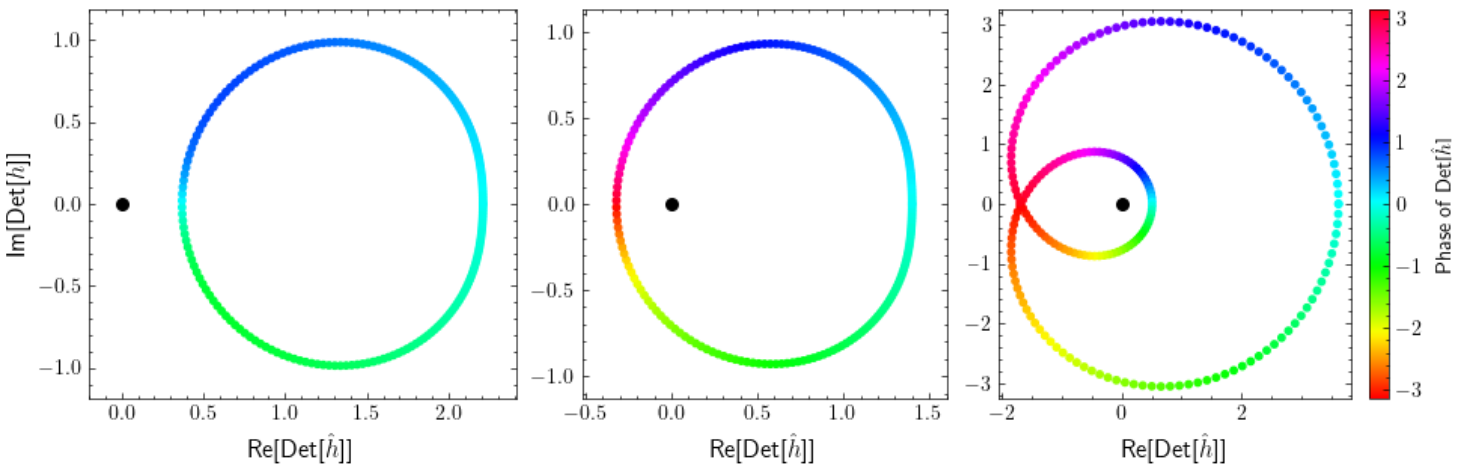
\includegraphics[width=\linewidth]{media/sp-ssh-012.png}
	\caption[Topology of the SP-SSH lattice for $\Delta\beta = 0$.]{Topology of the SP-SSH lattice for $\Delta\beta = 0$. Determinant of the block matrix $\hat{h}$ for quasimomenta $-\frac{\pi}{a} \le k  < \frac{\pi}{a}$. Exactly three distinct topological phases are observed. \label{fig:sp-wilson}}
\end{figure} \vspace{-8ex}
To obtain the full phase diagram (particularly for $\Delta \beta \neq 0$), it is sufficient to vary $\Delta \beta$ and observe when band gap closure occurs, as shown in Figure~\ref{fig:sp-ssh-phase-diagram}. The SP-SSH lattice exhibits two topological mechanisms: one due to SP hybridization and another due to dimerization.
\begin{figure}[H]
	\centering
	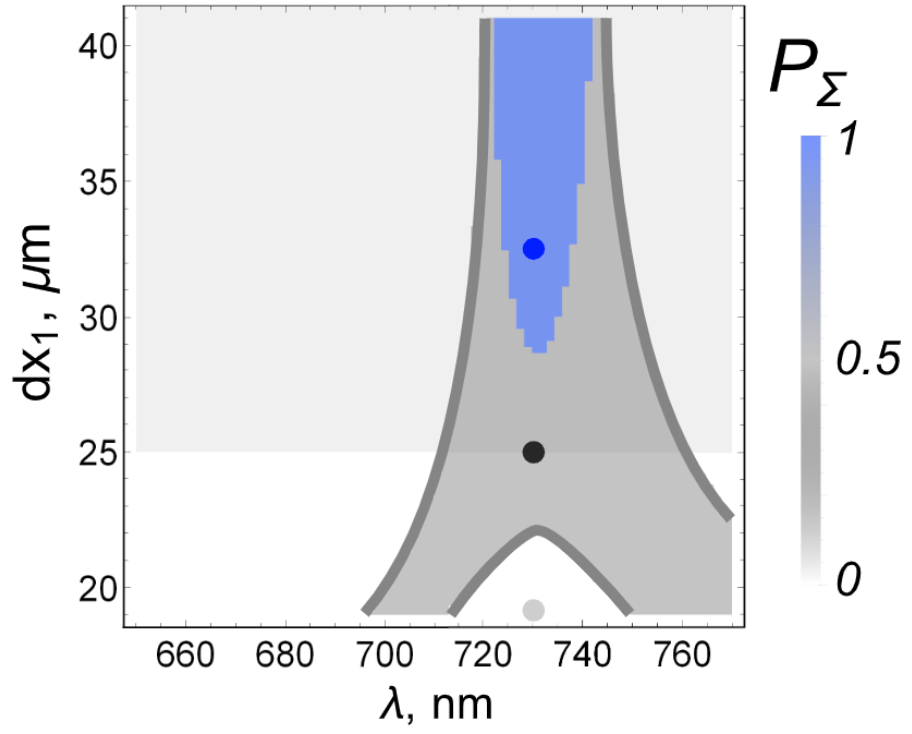
\includegraphics[width=0.6\linewidth]{media/sp-ssh-phase-diagram.png}
	\caption{Topological phase diagram. \label{fig:sp-ssh-phase-diagram}}
\end{figure} \vspace{-2ex}
\section{Experimental Implementation}
To experimentally implement the SP-SSH model, 25 photonic lattices were fabricated using the femtosecond laser writing technique described in Chapter~\ref{cap:fs}. The geometric parameters were adjusted with separations between molecules: variable $dx_1$, $dx_2 = 25$ $\mu$m, $dy = 20$ $\mu$m nd between waveguides: $dx_0 = 7$ $\mu$m. The refractive index contrasts were optimized to achieve mode degeneracy: $k_z^S \sim k_z^P$ at $\lambda = 730$ nm \cite{interorbital}. Measurements were performed via wavelength scanning (Chapter~\ref{cap:wavelength}) with $\lambda \in$ $\{700, 780\}$ nm and a step of 5 nm, aiming to control the parameter $\Delta \beta$, which depends directly on the wavelength used. Excitation was applied to the $S$ waveguide at one end of the lattice, measuring the relative power at the same end ($I_{\text{edge}}/I_{\text{total}}$). Although the topological phases with bulk polarization\footnote{topological invariant that allows distinguishing different topological phases.} $P_\Sigma=1/2$ or $P_\Sigma=1$, are not initially clearly distinguishable, numerical analysis reveals that during the second topological transition the ratio $I_{\text{edge}}/I_{\text{total}}$ should form a plateau. Figure~\ref{fig:sp-ssh-num} confirms this behavior, while Figure~\ref{fig:sp-ssh-exp} shows representative experimental results: one for $\lambda =$ 680 nm, where only dimerization-induced topology is observed, and another for $\lambda =$ 725 nm, where two topological transitions occur as dimerization changes.

\begin{figure}[H]
	\centering
	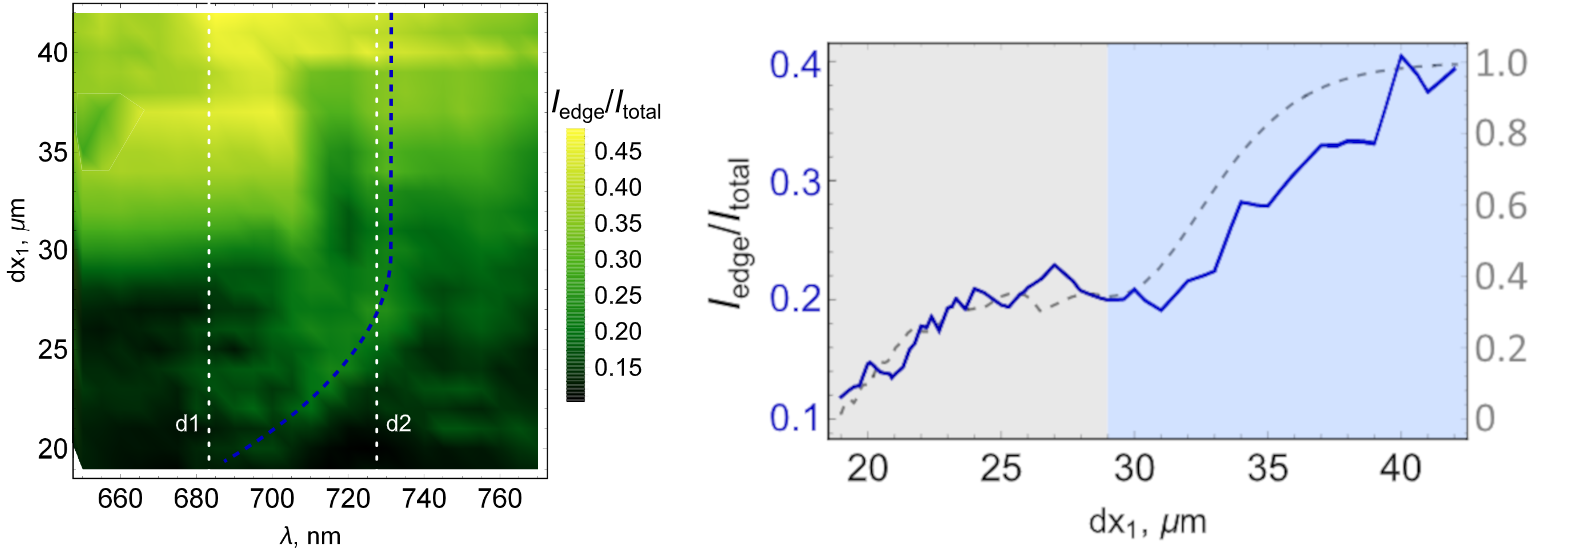
\includegraphics[width=0.9\linewidth]{media/sp-ssh-exp-num.png}
	\caption[Numerical-experimental analysis of the SP-SSH model]{
		\textbf{Left:} Experimental results showing the characteristic plateau.
		\textbf{Right:} Quantitative comparison between experimental data (solid line) and simulations (dashed line).
		\label{fig:sp-ssh-num}}
\end{figure}

\begin{figure}[H]
	\centering
	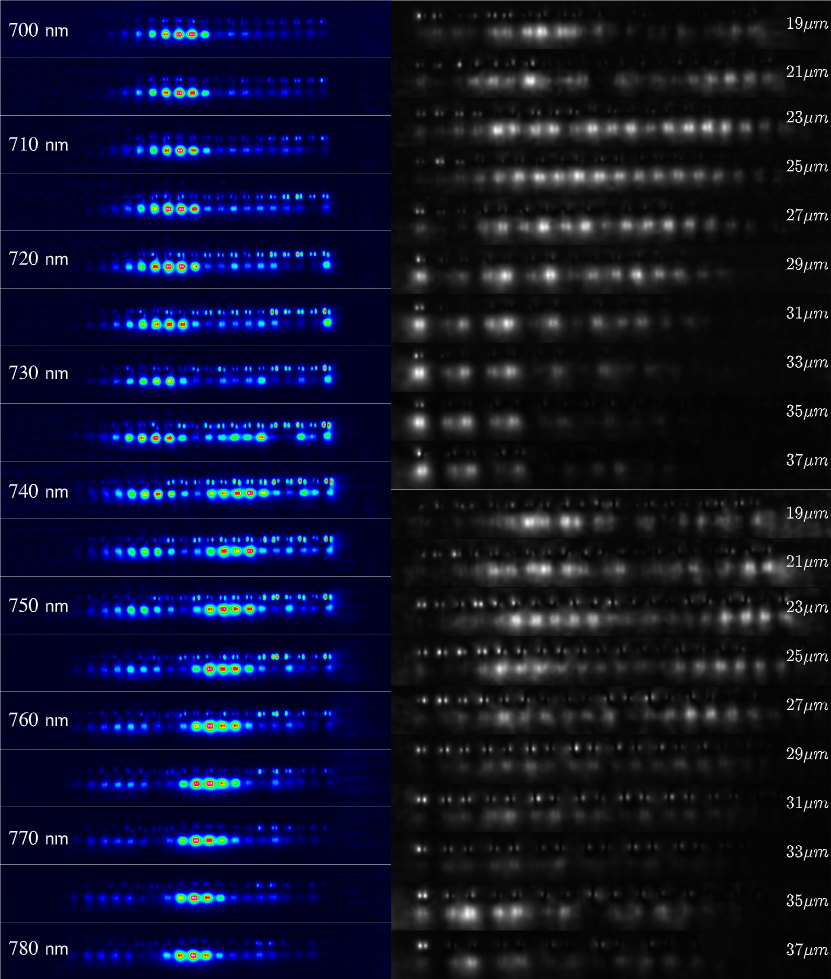
\includegraphics[width=\linewidth]{media/sp-ssh-exp.png}
	\caption[Experimental characterization of SP-SSH lattices]{
		\textbf{Left:} Homogeneous SP-SSH lattice ($dx_1 = dx_2$) for different wavelengths.
		\textbf{Right:} Top: Excitation at 680 nm for different dimerizations.
		Bottom: Same excitation at 725 nm.
		\label{fig:sp-ssh-exp}}
\end{figure}


\chapter{Conclusions}
\label{cap:conclu}

This thesis has systematically investigated the properties of discrete photonic lattices with non-conventional transverse modes, focusing on configurations that include \( P \) modes, \( S\hspace*{-0.3ex}P \)inter-orbital couplings, and non-symmetric evanescent couplings. The research combined analytical tools, numerical simulations, and experimental validation to address different manifestations of the orbital structure of guided light.

In Chapter~\ref{cap:invisibility}, a honeycomb-type photonic lattice composed of \( p_y \) modes was characterized, demonstrating that the \textit{invisibility angle} induces a quasi-flat band regime around \( \theta \approx 0.56 \) radians. Through a detailed analysis incorporating non-orthogonality corrections and long-range couplings, it was established that Aharonov-Bohm-type confinement persists even in the presence of these perturbations. In particular, it was confirmed that non-orthogonality effects are essential to correctly describe localization at the lattice edges, which was quantified using the inverse participation ratio (IPR) and experimentally corroborated.

Chapter~\ref{cap:asymmetric} addressed the phenomenon of non-symmetric evanescent coupling in photonic dimers with different refractive index contrasts. A generalization of coupled-mode theory was presented, including non-orthogonality terms, which allows correct modeling of the observed directional dynamics. Experimentally, an energy transfer imbalance dependent on the input channel was verified, in agreement with theoretical predictions based on non-symmetric effective coupling matrices.

In Chapter~\ref{cap:molecules}, the implementation of SP-SSH lattices constructed from photonic molecules was studied. It was demonstrated that structural dimerization, combined with hybridization between \( S \) and \( P \) modes, gives rise to two independently controllable topological phase transitions. Phases with different quantized bulk polarizations were identified, and an experimental protocol was designed to detect edge modes through the ratio \( I_{\text{borde}} / I_{\text{total}} \)in excellent agreement with numerical simulations. This model extends the physics of the one-dimensional SSH system to the multi-orbital context, revealing new mechanisms of topological localization mediated by internal degrees of freedom.

From a methodological perspective, this thesis developed a continuous numerical method based on eigenmode expansion (EME), which extends coupled-mode theory to the regime of closely spaced waveguides or arbitrary refractive index contrasts. This approach was complemented by experimental techniques for fabricating and characterizing multi-orbital lattices, enabling the calibration of propagation constants for distinct guided modes.

The obtained results open new possibilities for designing photonic devices that exploit localization and control mechanisms based on geometry, transverse symmetry, and topology. Furthermore, a theoretical-experimental framework adaptable to more complex platforms is established, for example, in systems with orbital angular momentum \citep{OAMCaging}.


% ver https://www.overleaf.com/learn/latex/Glossaries
% \input{glosario.tex} % opcional

%\nocite{*}
\bibliographystyle{unsrtnat}
\bibliography{citations}

% Set appendix section numbers as "Anexo A"
%\renewcommand{\appendixname}{Anexo}
\renewcommand{\thesection}{\appendixname~\Alph{section}}
% Appendices section
\begin{minipage}{\textwidth}
\chapter*{Appendices}
\markboth{Anexos}{Anexos}

% --- Fix blank page & TOC hyperlink ---
\clearpage % Ensure bibliography ends properly
\phantomsection % Fixes hyperref link for the appendix
\addcontentsline{toc}{chapter}{Anexos}
\appendix
	\setcounter{section}{0} % Reset counter
	\nopagebreak
	\section{\qquad Papers published in chronological order}
\begin{figure}[H]
	\centering
	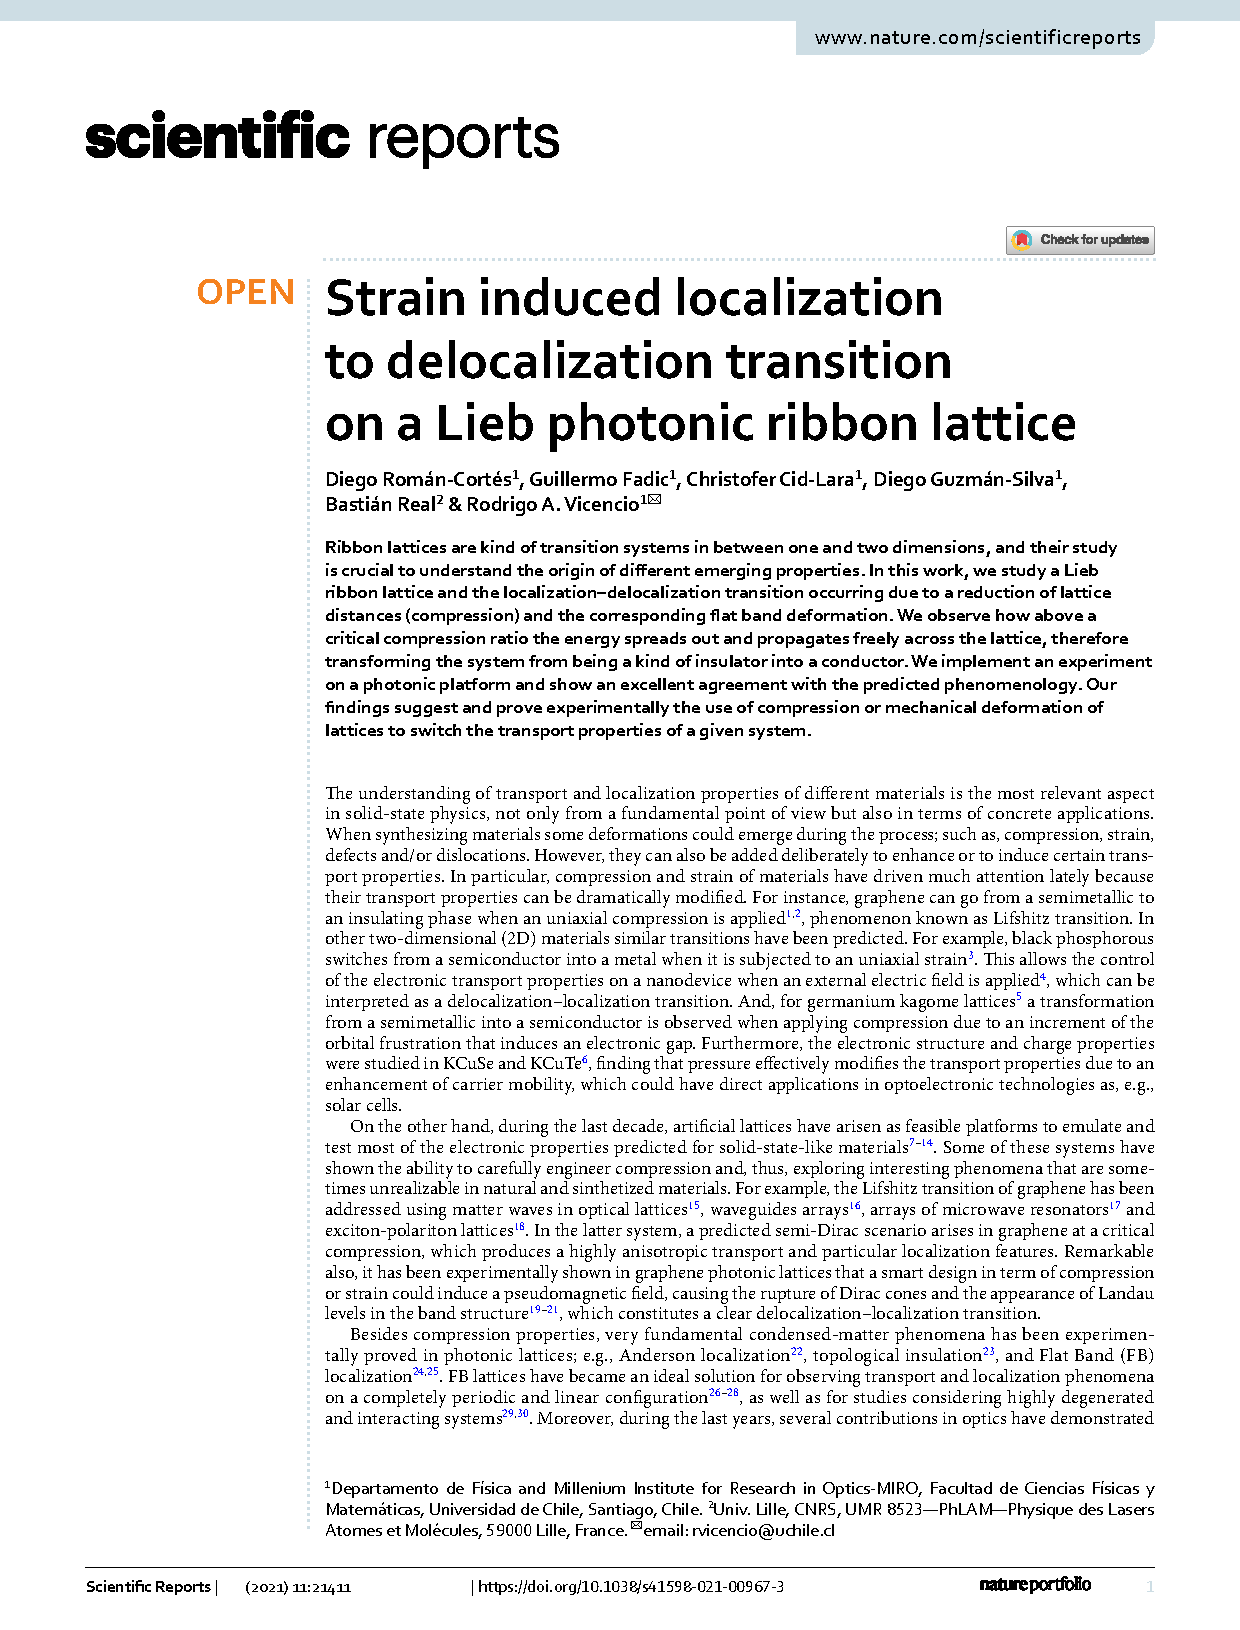
\includegraphics[page=1, width=0.9\linewidth]{media/strainlieb.pdf}
\end{figure}

\end{minipage}
\newpage
\begin{figure}[H]
	\centering
	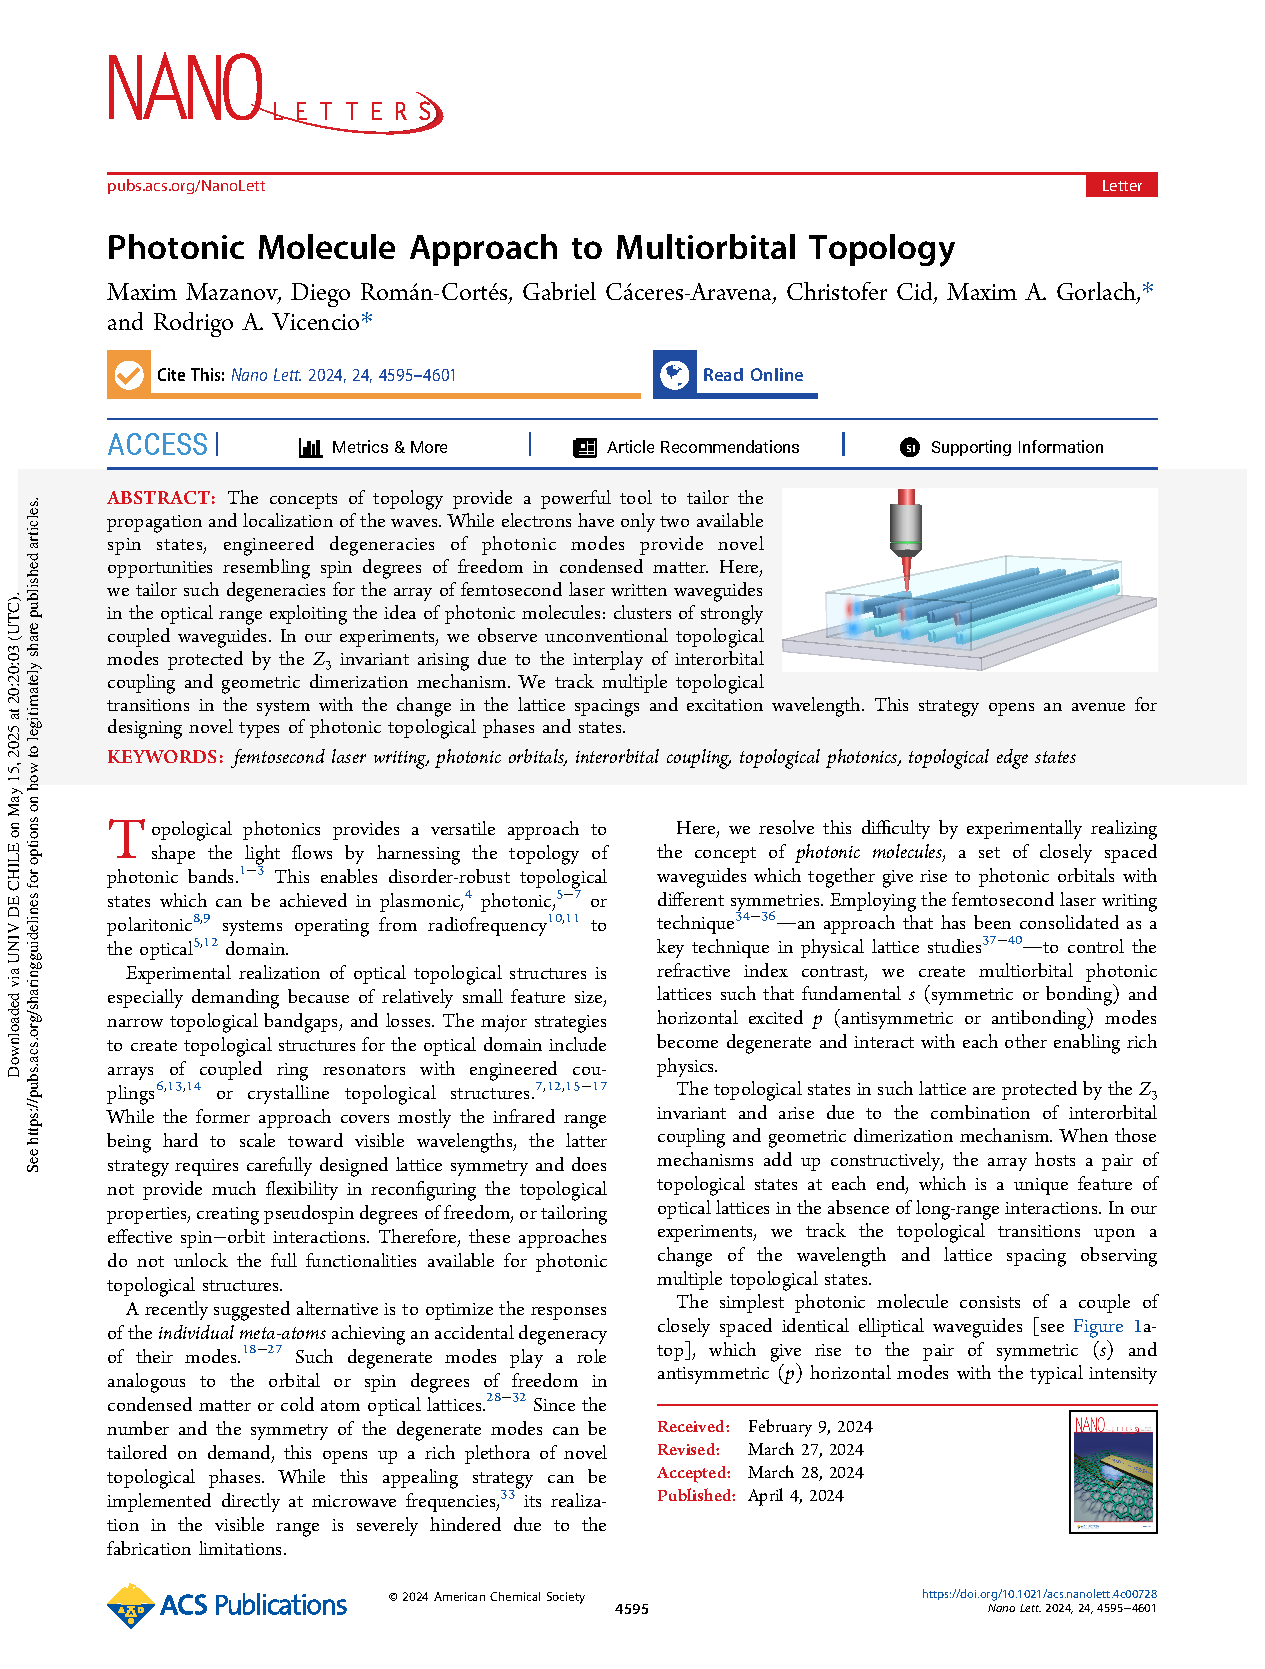
\includegraphics[page=1, width=\linewidth]{media/molpap.pdf}
\end{figure}
\begin{figure}[H]
	\centering
	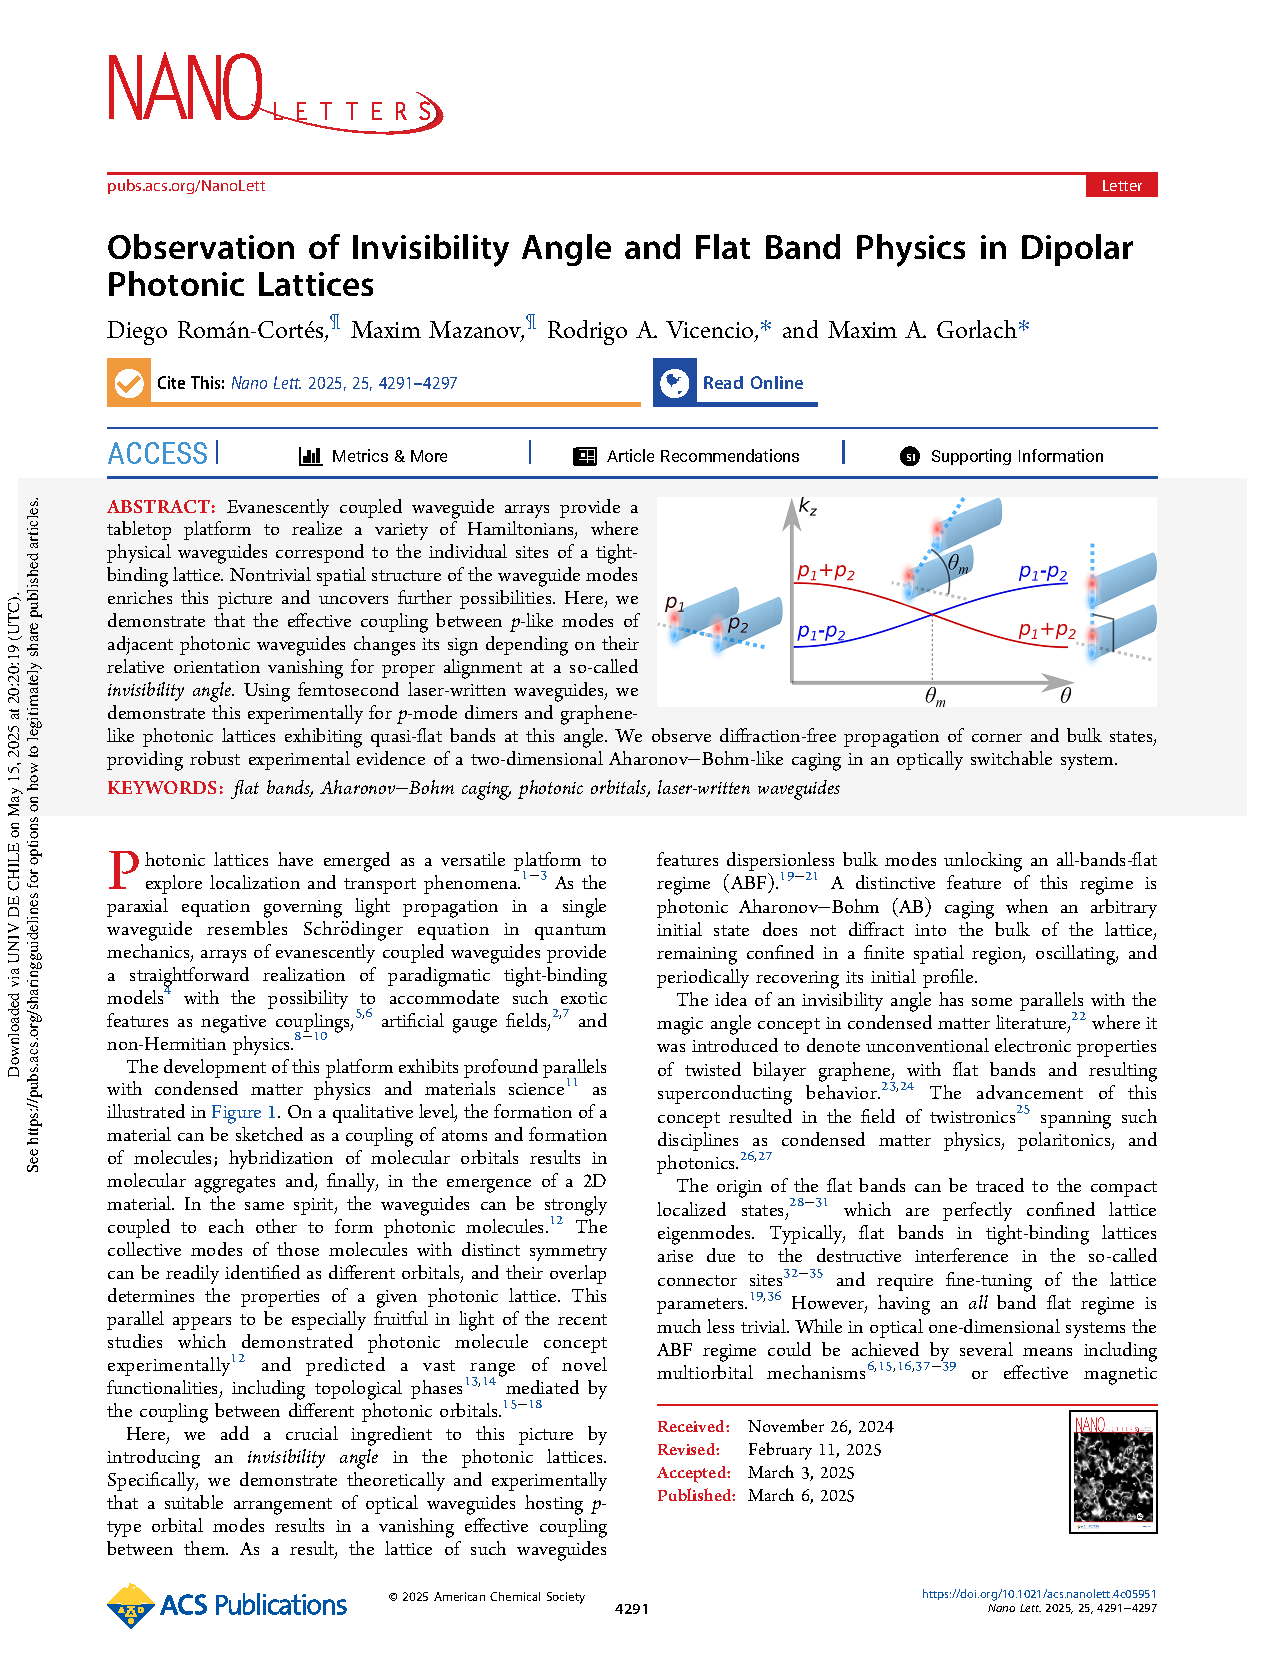
\includegraphics[page=1, width=\linewidth]{media/dipolepap.pdf}
\end{figure}
\begin{figure}[H]
	\centering
	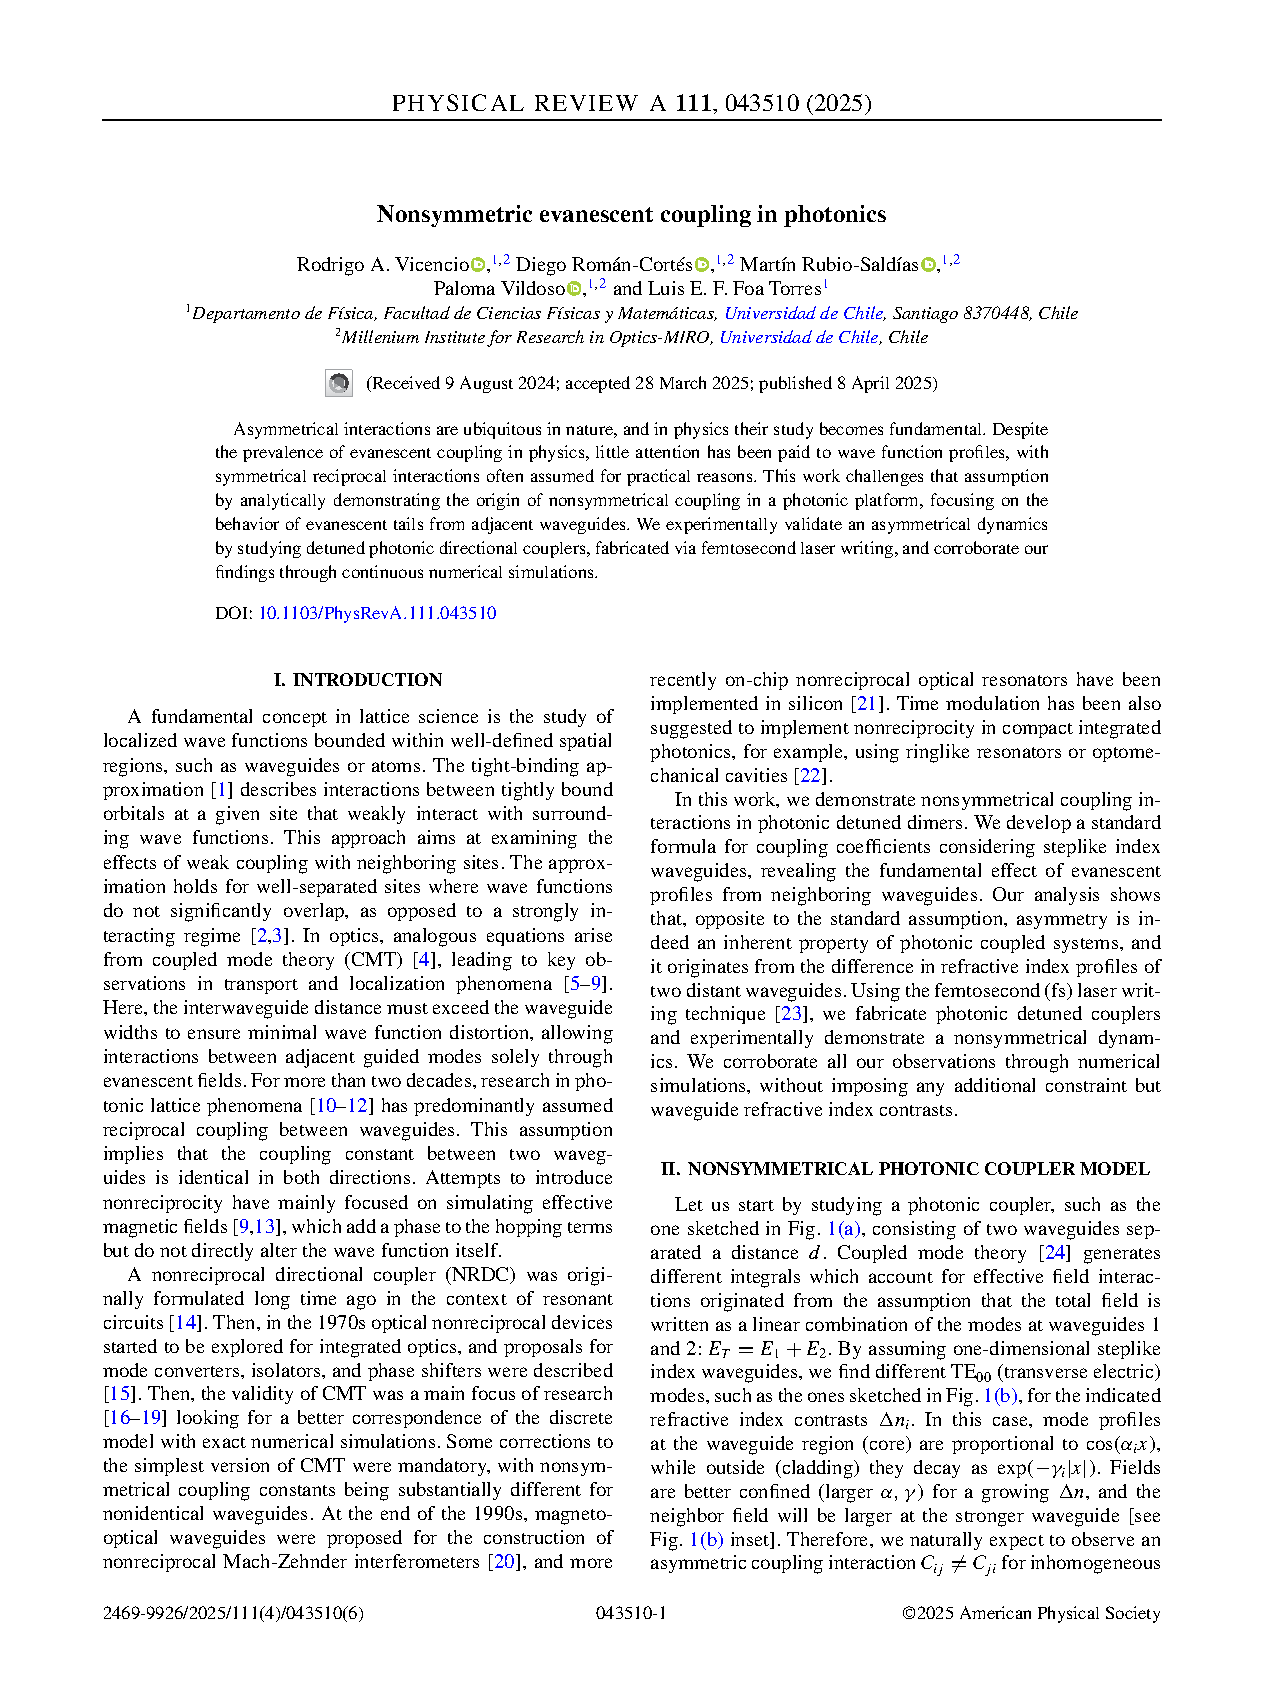
\includegraphics[page=1, width=\linewidth]{media/nonsympap.pdf}
\end{figure}
\begin{figure}[H]
	\centering
	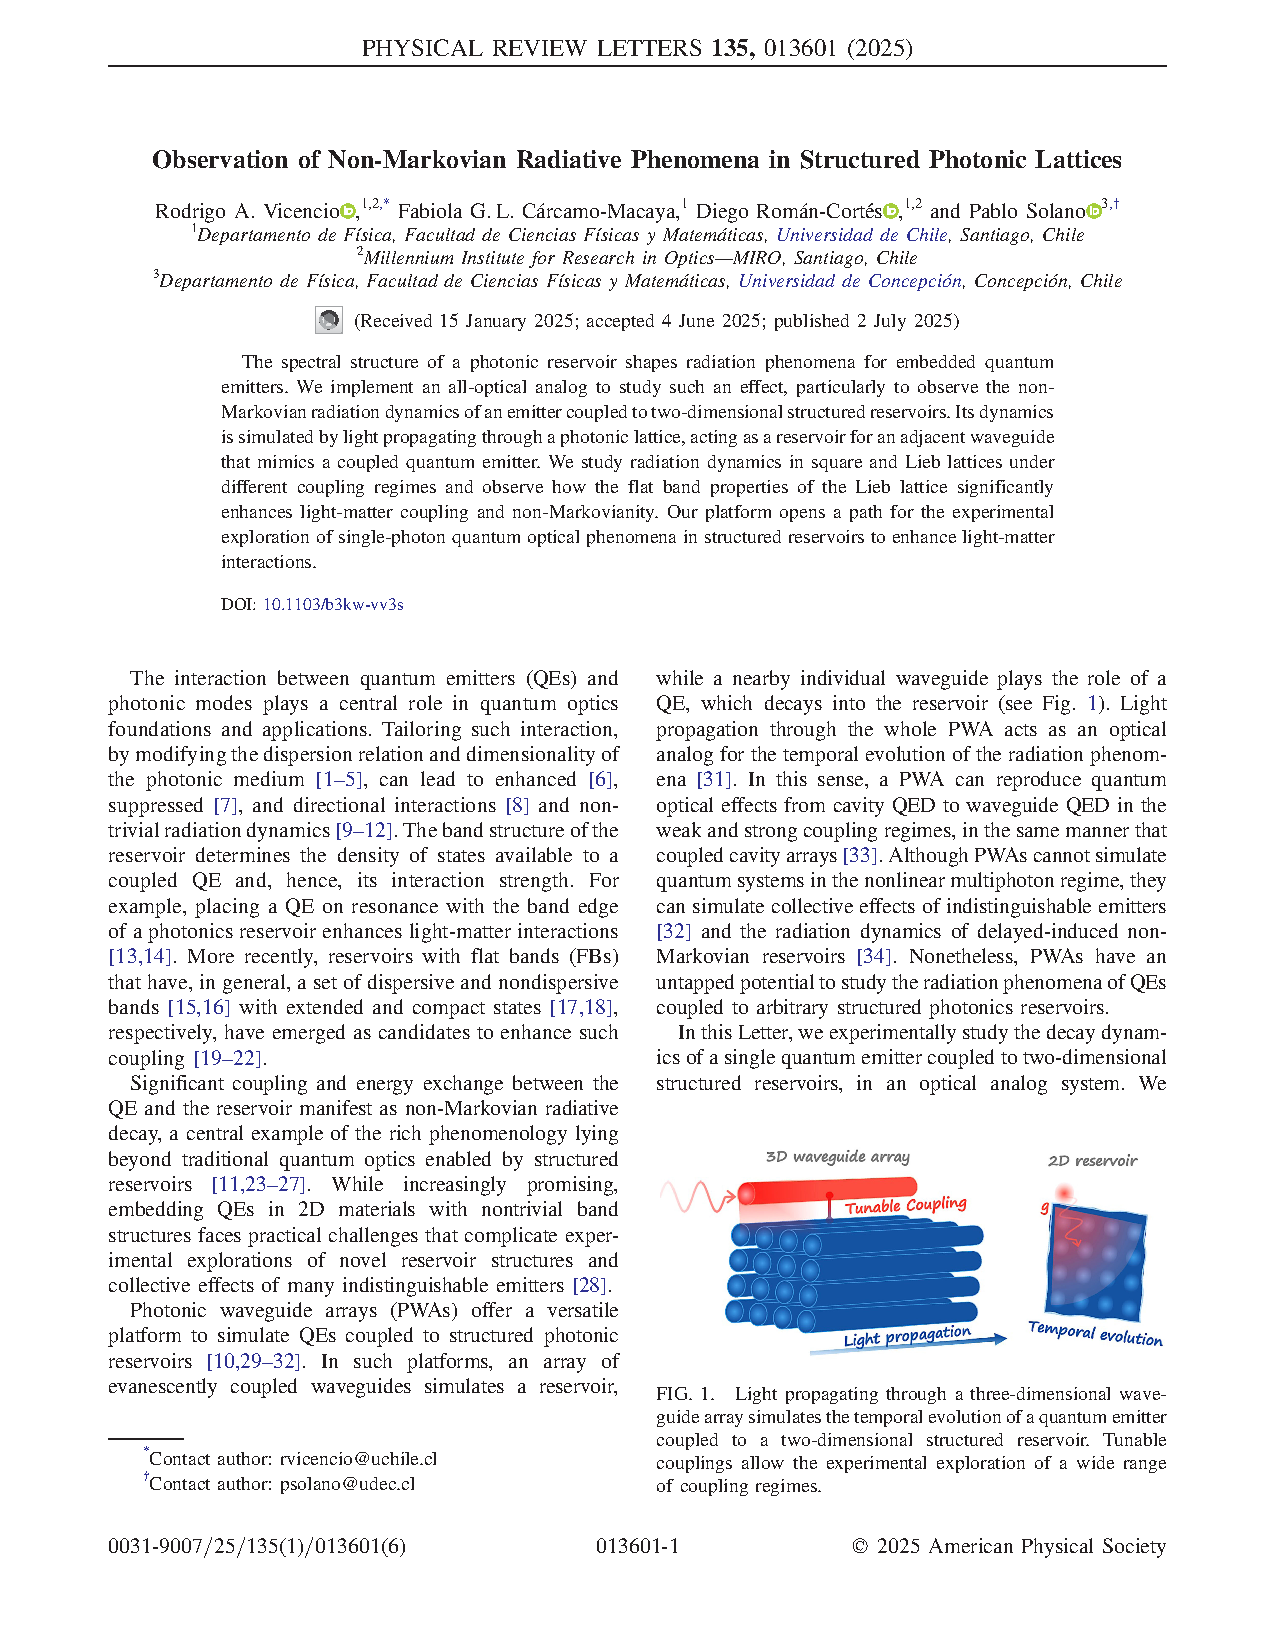
\includegraphics[page=1, width=\linewidth]{media/2Dradpap.pdf}
\end{figure}
	\section{\qquad Orthogonality of the normal modes \label{sec:orto}}

The orthogonality of the normal modes $\textbf{E}_\nu^\perp$ can be demonstrated using the Einstein convention in equation (\ref{eqn:eigenfield}) to simplify the notation:
\begin{equation}
	T_{ij} E^\nu_j = \beta_\nu^2 E^\nu_i, \label{eqn:eigentensorial}
\end{equation}
where the operator $T_{ij}$ acts as $T_{ij}E_j \equiv \delta_{ij}\left(\nabla_\perp^2 + k_0^2n^2\right)E_j + \partial_i \left(E_j \partial_j\ln(n^2)\right).$

To demonstrate the orthogonality of the modes $E_i$,  it can be equivalently shown that $T_{ij}$ is Hermitian:
\begin{align}
	\iint \left(T_{ij} E_j^\mu\right)^* E_i^\nu \,dA = \iint \left(E_i^\mu\right)^* \left(T_{ij} E_j^\nu\right) \,dA.
\end{align}
This property follows from the identity:
\begin{align*}
	&\left(T_{ji} E_i^\mu\right)^* E_j^\nu - \left(E_i^\mu\right)^* \left(T_{ij} E_j^\nu\right) =  \nabla_\perp \cdot \left[E_i^\nu \nabla_\perp \left(E_i^\mu\right)^* - \left(E_i^\mu\right)^* \nabla_\perp E_i^\nu\right]  + \left[E^\nu_j \partial_j \left(E_i^\mu\right)^* - \left(E_j^\mu\right)^* \partial_j E_i^\nu\right] \partial_i \ln(n^2).
\end{align*}
When integrating over the transverse plane, the divergence term vanishes for guided modes (which decay at infinity), but the second term disappears only if $\nabla n^2 = \textbf{0}$. That is, the operator $T_{ij}$ is Hermitian only under the weak guidance condition.

The complete system is Hermitian, as demonstrated by starting from the equation (\ref{eqn:rotordoble}):
\begin{align*}
	\iiint_V \left(\nabla\times\nabla\times\textbf{E}^\nu\right) \cdot \left(\textbf{E}^\mu\right)^* dV &= \iiint_V n^2\frac{\omega_\nu^2}{c^2} \textbf{E}^\nu \cdot \left(\textbf{E}^\mu\right)^* dV \\
	\iiint_V \left[\nabla\times\nabla\times\left(\textbf{E}^\mu\right)^*\right] \cdot \textbf{E}^\nu dV &= \iiint_V n^2 \frac{\omega_\mu^2}{c^2} \left(\textbf{E}^\mu\right)^* \cdot \textbf{E}^\nu dV
\end{align*}

Subtracting both equations and applying the divergence theorem:
\begin{align*}
	\frac{\omega_\nu^2 - \omega_\mu^2}{c^2} \iiint_V n^2 \textbf{E}^\nu \cdot \left(\textbf{E}^\mu\right)^* dV &= \oiint_{\partial V} \left[ \cdots \right] \cdot \hat{\textbf{n}}\,dA \\
	&\xrightarrow{\partial V \to \infty} 0
\end{align*}
This yields two possibilities: either the modes are degenerate ($\omega_\nu^2 = \omega_\mu^2$), or we have $\iiint n^2 \textbf{E}^\nu \cdot \left(\textbf{E}^\mu\right)^* dV = 0$.
	\input{anexoB.tex}
	\newpage
	\section{\qquad BPM C code \label{sec:codigoBPM}}

\lstinputlisting[language=C]{./codigo/array1d.c}
	\newpage
	\section{\qquad Hologram generator Python code \label{sec:codigoSLM}}

\lstinputlisting[language=Python]{./codigo/slm_blaze.py}

\end{document}